\documentclass[12pt]{book}
\usepackage[utf8]{inputenc}
\usepackage[T1]{fontenc}
\usepackage{geometry}
\geometry{a4paper, margin=1in, bindingoffset=0.35in}
\usepackage{newtxtext}
\usepackage{newtxmath}
\usepackage{microtype}
\emergencystretch=2em
\usepackage{graphicx}
\usepackage{tabularx}
\usepackage{enumitem}
\usepackage{xcolor}
\usepackage{fancyhdr}
\setlength{\headheight}{14.5pt}
\usepackage{setspace}
\setstretch{1.15}
\usepackage[hidelinks]{hyperref}
\usepackage{tikz}
\usepackage{makeidx}
\makeindex

\pagestyle{fancy}
\fancyhf{}
\fancyhead[LE]{\small\nouppercase{\leftmark}}
\fancyhead[RO]{\small\nouppercase{\leftmark}}
\fancyfoot[C]{\small\thepage}
\renewcommand{\headrulewidth}{0.4pt}

\newcommand{\quicknote}[1]{\noindent\textbf{Note:} #1\par\vspace{0.5em}}

\title{\textbf{\Huge FIRST AID}\\[1em]\Large A Comprehensive First Aid Reference Manual\\[0.5em]\small First Edition\\[0.3em]\small Following the 2024 AHA/ARC First Aid Guidelines, ILCOR 2025, and ERC Guidelines 2025}
\author{Chaman Singh Verma}
\date{\today}

\begin{document}

\frontmatter
\maketitle

\setcounter{tocdepth}{1}
\tableofcontents

\clearpage

\section*{Preface}

This reference provides first aid guidance for the Indian lay responder, based on current evidence-based protocols from leading international health organizations, including the 2024 American Heart Association / American Red Cross First Aid Guidelines, the 2025 International Liaison Committee on Resuscitation (ILCOR) Consensus on Science with Treatment Recommendations, the 2025 European Resuscitation Council Guidelines, and the World Health Organization (WHO) First Aid Guidelines (2018). It is designed for people without medical training who want clear, actionable information on managing common injuries and emergencies before professional medical help arrives — whether at home, at work, on the road, or in the field.

\textbf{Purpose and Scope}

The content covers practical, step-by-step management of the most frequently encountered first aid scenarios in the Indian context — from bleeding control and wound care to cardiac events, respiratory distress, environmental injuries, snakebite, heat-related illness, and toxic exposures. Emergency numbers, Good Samaritan protections, disaster preparedness, and poison control guidance are given for India (dial 112 or 108 for emergency ambulance services), while noting that local numbers vary by state. Emphasis is placed on recognizing when professional medical care is required and what actions can safely be performed at the scene.

\textbf{How to Use This Reference}

Each section follows a consistent structure: recognition of signs and symptoms, immediate first aid actions, warning signs indicating escalation to emergency care, and important contraindications (what not to do). Quick-reference warnings and notes highlight critical safety points. Turn to the relevant chapter by injury type or clinical presentation.

\textbf{Important Disclaimer}

This material is for informational and educational purposes only and does not constitute medical advice, diagnosis, or treatment. First aid should never replace professional medical evaluation or care when indicated. Always seek qualified medical attention for serious injuries, persistent symptoms, or uncertain situations. Laws, regulations, and available resources vary across states and regions; consult local health authorities, the National Health Mission, and certified first aid training programs for region-specific guidance.

No person should perform any procedure beyond their level of training and comfort. When in doubt, call emergency services immediately.

\textbf{Acknowledgments}

This work draws upon authoritative sources including the 2024 AHA/ARC First Aid Guidelines, the 2025 ILCOR CoSTR, the ERC Guidelines 2025, World Health Organization, American Heart Association, American Red Cross, the Indian Red Cross Society \cite{ircs}, the National Disaster Management Authority (NDMA) \cite{ndma}, the National Poisons Information Centre (AIIMS New Delhi) \cite{npic}, the Supreme Court of India's Good Samaritan guidelines \cite{sc_goodsam}, Centers for Disease Control and Prevention, and national poison control centers. Special thanks to first responders, emergency physicians, and public health educators whose expertise informed the content development.

We welcome feedback and corrections. Please contact the authors with any suggestions for improvement.


\mainmatter

\chapter{Introduction to First Aid}\label{ch:introduction}

\section{What is First Aid?}

First aid is the immediate care given to a person who has been injured or taken suddenly ill, provided on the spot before professional help arrives. It is not a substitute for a doctor but the help that buys time when every minute counts. It covers physical support, such as controlling bleeding, and emotional support, such as reassuring the person, and can mean the difference between life and death, full recovery and permanent injury, or a worsening condition. This chapter explains the purposes, responsibilities, and limits of first aid.

The basic purposes of first aid are:

\begin{itemize}[leftmargin=*]
  \item To preserve life
  \item To prevent further harm or deterioration of the condition
  \item To promote recovery
\end{itemize}

\section{When Should First Aid Be Administered?}

First aid should be provided in any situation where an individual needs emergency care but professional medical help is not immediately available or en route. Common scenarios include:

\begin{itemize}[leftmargin=*]
  \item Trauma from accidents (vehicle collisions, falls, sports injuries)
  \item Medical emergencies (heart attacks, strokes, seizures, diabetic episodes)
  \item Environmental conditions (heat stroke, hypothermia, drowning)
  \item Poisonings and exposures (chemical, drug, venomous bites)
  \item Burns and scalds
  \item Choking incidents
  \item Bleeding from wounds
\end{itemize}

\section{The Chain of Survival}

For cardiac arrest and other life-threatening situations, the American Heart Association emphasizes the "Chain of Survival" \cite{aha_bls_2020,ilcor_2025}:

\begin{enumerate}[leftmargin=*]
  \item Immediate recognition of cardiac arrest and activation of emergency response system
  \item Early cardiopulmonary resuscitation (CPR) with emphasis on chest compressions
  \item Rapid defibrillation when available
  \item Advanced life support by healthcare professionals
  \item Post-cardiac arrest care
\end{enumerate}
Each link in this chain must be in place quickly and effectively to maximize the chance of survival.

\section{Legal Protection for First Aiders}

In India, Good Samaritan laws protect individuals who provide reasonable first aid in good faith from liability. In \textbf{March 2016}, the Supreme Court of India (Raj Kumar v.\ State of NCT of Delhi) laid down binding guidelines protecting Good Samaritans from civil and criminal liability arising from their efforts to help road accident victims \cite{sc_goodsam}. This protection was subsequently given statutory backing through \textbf{Section 134A} of the Motor Vehicles Act, 1988, and the Good Samaritan Rules, 2022, issued by the Ministry of Road Transport and Highways. Under these provisions:

\begin{itemize}[leftmargin=*]
  \item A Good Samaritan who assists an accident victim is not liable for any civil or criminal action for injury or death caused by their actions in good faith
  \item Police and hospital staff are not permitted to compel a Good Samaritan to disclose their name, address, phone number, or any personal details
  \item A Good Samaritan is not required to become a witness or to take the injured person to a hospital
  \item Hospitals are required to provide immediate basic emergency medical care to accident victims regardless of the victim's ability to pay
\end{itemize}

These protections typically require that:

\begin{itemize}[leftmargin=*]
  \item The helper acts voluntarily (not expecting payment)
  \item The helper provides care within their level of training
  \item The helper does not act recklessly or with gross negligence
  \item Consent is obtained when possible (implied consent is assumed in emergencies involving unconscious persons)
\end{itemize}

The Good Samaritan guidelines apply in addition to the general legal principle that a person who acts reasonably and in good faith is not penalized for doing so. Laws vary by jurisdiction within India, so it is important to understand local legislation.

\quicknote{\textbf{Safety First}: Before approaching anyone who is injured or ill, always ensure your own safety. Do not become another victim. Check the scene for dangers such as traffic, fire, hazardous materials, electrical hazards, or violence.}

\section{Getting Started: A Simple Protocol}

When responding to any emergency, follow these basic steps:

\begin{enumerate}[leftmargin=*]
\item Assess the Scene -- Ensure your safety and check for hazards
\item Check Responsiveness -- Gently tap and shout ``Are you OK?''
\item Call for Help -- If unresponsive, call emergency services immediately. In India, dial \textbf{112} (the national emergency number) or \textbf{108} (emergency ambulance in many states); \textbf{100} for police and \textbf{101} for fire
\item Provide Care -- Administer appropriate first aid based on the situation
\item Monitor Continuously -- Stay with the person until professional help arrives or they show signs of improvement
\end{enumerate}
\medskip\noindent\textbf{Quick Reference.}
Begin every first aid situation by prioritizing YOUR OWN SAFETY above all else. Never put yourself at risk when helping others. If the scene is unsafe, retreat and call emergency services from a safe location.

\section{Important Limitations}

This book provides general information about first aid procedures. It is not a substitute for:

\begin{itemize}[leftmargin=*]
  \item Formal first aid certification courses (recommended annually)
  \item Professional medical evaluation and treatment
  \item Emergency medical services when needed
\end{itemize}

Always err on the side of caution. When in doubt, seek professional medical assistance immediately.

\section{Psychological First Aid}

Injuries and emergencies are frightening, and emotional distress is as real as physical pain. Psychological first aid means offering calm, practical support without trying to "fix" feelings or force the person to talk. It can be given by anyone.

\begin{itemize}[leftmargin=*]
  \item \textbf{Stay calm and present}: Speak in a calm, steady voice. Introduce yourself and say what you are doing before you touch or treat the person
  \item \textbf{Make the environment feel safer}: Move to quieter, calmer surroundings when possible; protect the person from further exposure to the distressing scene
  \item \textbf{Listen without judgment}: Let the person talk if they want to. Do not minimize their feelings (avoid "it's not that bad") and do not force them to describe details
  \item \textbf{Offer practical help}: Provide water, warmth, and information about what is happening and what will happen next. Simple, honest reassurance reduces anxiety
  \item \textbf{Support connections}: Ask if there is someone they would like contacted -- family, a friend, or a support person
  \item \textbf{Watch for concerning reactions}: Severe agitation, panic, confusion, withdrawal, or the person being unable to care for themselves may need professional mental health support. People who have experienced trauma, including rescuers themselves, may need follow-up care days or weeks later
\end{itemize}

\quicknote{\textbf{Children}: Children often react more strongly than adults. Keep explanations brief and age-appropriate, stay close and reassuring, and return them to a familiar adult or routine as soon as possible.}

\quicknote{\textbf{Rescuers}: Looking after your own well-being matters. Debriefing with someone you trust after a stressful incident is normal and healthy -- including for trained responders.}

\section{References}

This book draws on the current international first aid and resuscitation guidelines cited throughout the text. Full bibliographic details appear in the Bibliography at the end of this book. Key sources include the 2024 AHA/ARC First Aid Guidelines \cite{aha_arc_2024}, the 2025 ILCOR Consensus on Science with Treatment Recommendations \cite{ilcor_2025}, the ERC Guidelines 2025 \cite{erc_2025}, and supporting references from the American Red Cross \cite{arc_2020}, the World Health Organization \cite{who_2018}, and the Centers for Disease Control and Prevention \cite{cdc}.

\section{Review Questions}

\begin{enumerate}[leftmargin=*]
\item What are the three basic purposes of first aid?
\item List the links of the Chain of Survival in order.
\item What four conditions typically protect a Good Samaritan from liability?
\item What is the very first step in any emergency response, and why?
\item A person is unresponsive and not breathing normally. What two actions do you take, in what order?
\end{enumerate}
\index{first aid}
\index{emergency response}
\index{Good Samaritan law}
\index{chain of survival}
\index{psychological first aid}
\index{emotional support}
\chapter{Basic First Aid Principles}\label{ch:basic_principles}

\section{Infection Control and Personal Protection}

Preventing the transmission of disease is a fundamental principle in first aid. Always take precautions to protect both yourself and the person receiving care.

\subsection{Standard Precautions}

Treat all blood and body fluids as potentially infectious. Follow these standard precautions \cite{cdc,who_2018}:

\begin{enumerate}[leftmargin=*]
  \item Wash hands thoroughly with soap and water before and after providing care, or use alcohol-based hand sanitizer (at least 60\% alcohol) if soap and water are unavailable
  \item Wear disposable gloves when there is contact with blood, open wounds, or body fluids
  \item Use protective equipment such as face shields, masks, or goggles when splashing is possible
  \item Avoid direct skin-to-skin contact with open wounds
  \item Dispose of contaminated materials safely in sealed plastic bags
  \item Clean any exposed skin areas immediately with soap and water
\end{enumerate}
\quicknote{\textbf{Glove Usage}: Never reuse disposable gloves. If gloves become torn or punctured during use, remove them immediately and replace with a new pair.}

\section{Assessing Responsiveness}

The first step in any emergency assessment is determining whether the person is conscious and responsive.

\begin{enumerate}[leftmargin=*]
\item Approach the person from the front where they can see you
\item Tap both shoulders firmly and shout loudly: ``Can you hear me? Are you OK?''
\item Look for response: opening eyes, moving, speaking, or following simple commands
\end{enumerate}
\textbf{WARNING:} If there is NO response, call for help immediately and check for breathing and pulse (for unresponsive persons).

\section{Checking Breathing}

For an unresponsive person, checking breathing is critical.

\begin{enumerate}[leftmargin=*]
\item Place your ear near the person's mouth and nose while looking at their chest
\item Listen for breath sounds and feel for air movement on your cheek
\item Look for chest rise and fall over 5-10 seconds
\end{enumerate}
\textbf{WARNING:} If the person is NOT breathing or only gasping abnormally (agonal breaths), assume cardiac arrest and begin CPR immediately.

\section{Checking Pulse}

\textbf{Lay rescuers: do NOT perform a pulse check.} If a person is unresponsive and not breathing normally, assume cardiac arrest and begin CPR immediately -- pulse checks are unreliable in lay hands and delay chest compressions. The pulse check below is for trained or healthcare responders.

The carotid artery (neck) is the most accessible pulse point for adults.

\begin{enumerate}[leftmargin=*]
\item Place two fingers (not your thumb) on the side of the neck, just below the jaw angle
\item Press lightly against the trachea to find the carotid artery
\item Check for a pulse for no more than 10 seconds
\end{enumerate}
\quicknote{\textbf{Children and Infants}: For children up to puberty, use the brachial artery (inner upper arm). For infants (<1 year), also use the brachial artery or femoral artery (groin area).}

\medskip\noindent\textbf{Emergency Summary Table.}
\begin{center}
\begin{tabularx}{\textwidth}{@{}>{\raggedright\arraybackslash}X>{\raggedright\arraybackslash}X>{\raggedright\arraybackslash}X>{\raggedright\arraybackslash}X@{}}
\hline
\textbf{Condition} & \textbf{Response} & \textbf{Breathing} & \textbf{Action} \\
\hline
Responsive & Yes & Normal & Monitor, comfort, seek help if needed \\
Unresponsive & No & Normal & Place in recovery position, monitor continuously \\
Unresponsive & No & Not breathing/Only gasping & Begin CPR immediately (start compressions) \\
\hline
\end{tabularx}
\end{center}

\section{Positioning Unconscious Persons}

Proper positioning helps maintain airway patency and prevents aspiration.

\subsection{Recovery Position (Lateral Recumbent Position)}\label{sec:recovery_position}

Use this position for unconscious but breathing individuals to prevent choking on vomit or secretions.

\begin{enumerate}[leftmargin=*]
\item Kneel beside the person and extend their arm away from you at a right angle
\item Bend their other elbow and place the back of their hand against your cheek
\item Bring their far leg and bend it at the knee
\item Carefully roll them toward you using the bent leg as a pivot point
\item Tilt the head back slightly to keep the airway open
\item Ensure the top leg remains bent to stabilize the position
\end{enumerate}
\begin{figure}[h]
\centering
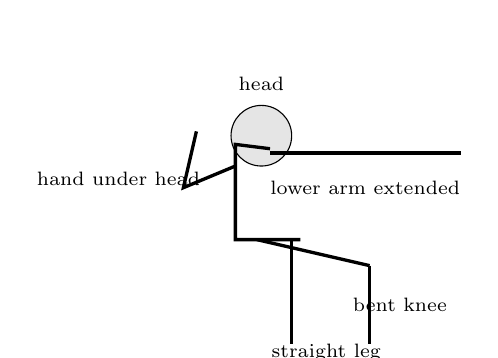
\begin{tikzpicture}[scale=1.1, >=stealth]
  \draw[fill=black!10] (0,0) circle (0.35);
  \node at (0,0.6) {\scriptsize head};
  \draw[very thick] (0.1,-0.2) -- (2.3,-0.2);
  \node at (1.2,-0.6) {\scriptsize lower arm extended};
  \draw[very thick] (0.1,-0.15) -- (-0.3,-0.1) -- (-0.3,-1.2) -- (0.45,-1.2);
  \draw[very thick] (-0.3,-0.35) -- (-0.9,-0.6) -- (-0.75,0.05);
  \node at (-1.65,-0.5) {\scriptsize hand under head};
  \draw[very thick] (0.35,-1.2) -- (0.35,-2.4);
  \node at (0.75,-2.5) {\scriptsize straight leg};
  \draw[very thick] (-0.05,-1.2) -- (1.25,-1.5);
  \draw[very thick] (1.25,-1.5) -- (1.25,-2.4);
  \node at (1.6,-1.95) {\scriptsize bent knee};
\end{tikzpicture}
\caption{Recovery position (viewed from above). The lower arm is extended on the ground, the upper arm's hand is tucked under the head, the near leg is straight, and the far leg is bent at the knee for stability.}
\label{fig:recovery_position}
\end{figure}

\textbf{WARNING:} Do NOT use the recovery position if you suspect spinal injury unless the person is vomiting or not breathing. In suspected spinal injuries, maintain manual in-line stabilization of the head and neck.

\section{Wound Assessment and Basic Care}

All wounds should be assessed quickly and systematically.

\subsection{Types of Wounds}

\begin{description}
  \item[Abrasion:] Scrape or raw surface caused by friction (road rash) that removes the outer layer of skin
  \item[Avulsion:] Partial or complete tearing away of skin and tissue
  \item[Contusion:] Bruise with intact skin but damaged underlying tissues
  \item[Laceration:] Cut or tear through skin and underlying tissue, often jagged edges
  \item[Puncture:] Small, deep wound caused by pointed objects (nails, needles, animal bites)
\end{description}

\subsection{Wound Management Steps}

\begin{enumerate}[leftmargin=*]
\item Ensure personal protection (wear gloves)
\item Control bleeding by applying direct pressure to the wound
\item Clean gently around the wound with sterile saline or clean water (avoid putting hydrogen peroxide or alcohol directly in the wound as it damages tissue)
\item Cover with a sterile dressing or bandage
\item Monitor for signs of infection (increased redness, warmth, swelling, pus, fever)
\end{enumerate}
\textbf{WARNING:} Seek immediate medical attention for: deep puncture wounds, animal/bite wounds, dirty wounds not cleaned within 8 hours, wounds with embedded objects, or signs of systemic infection.

\section{Basic Bandaging Techniques}

Proper bandaging supports healing without cutting off circulation.

\subsection{Glass Cuts}

Glass produces sharp, often clean lacerations that can be deeper than they appear. Special considerations include embedded fragments, tetanus risk, and stitch requirements.

\subsubsection{Initial Assessment}

\begin{itemize}[leftmargin=*]
  \item Assess bleeding severity — glass cuts may bleed steadily even if not spurting
  \item Look for visible glass fragments — use bright light and magnification if available
  \item Check depth — if the cut is deep enough to see fat, muscle, tendon, or bone, or if edges are gaping widely, seek medical evaluation for possible stitches
  \item Ask about tetanus vaccination status — a booster is recommended if the last shot was more than 5 years ago for dirty wounds like glass
\end{itemize}

\subsubsection{Managing Small Surface Fragments}

If small, visible glass fragments sit on the surface or just under the skin:

\begin{enumerate}[leftmargin=*]
  \item Wash your hands thoroughly and use clean tweezers (cleaned with alcohol if available)
  \item Gently lift or slide the fragment out in the direction it entered — do not dig deeply or enlarge the wound
  \item If the fragment is deeply embedded or you cannot remove it easily, DO NOT force it — cover with a sterile dressing and seek medical care
\end{enumerate}
\subsubsection{Wound Care After Fragment Removal}

\begin{enumerate}[leftmargin=*]
  \item Rinse the wound thoroughly with clean running water for several minutes to flush out any remaining tiny particles
  \item Clean gently around the wound with mild soap (avoid getting soap directly in the wound)
  \item Apply an over-the-counter antibiotic ointment (e.g., bacitracin or neomycin)
  \item Cover with a sterile adhesive bandage or non-stick dressing
  \item Change the dressing daily or whenever it becomes wet or soiled
\end{enumerate}
\subsubsection{When to Seek Medical Attention}

Seek professional care if:
\begin{itemize}[leftmargin=*]
  \item Bleeding continues after 10-15 minutes of steady direct pressure
  \item The wound is deeper than 1/4 inch (6 mm) or is gaping open
  \item You cannot remove all glass fragments
  \item Signs of infection develop (increasing redness, warmth, swelling, pus, fever)
  \item Numbness, tingling, or inability to move fingers/toes near the injury (possible nerve/tendon damage)
  \item The cut is on the face, hands, feet, or joints where precise closure matters
  \item Tetanus vaccination is unknown or outdated
\end{itemize}

\noindent\textbf{Note}: Unlike impaled glass (see Chapter~\ref{ch:bleeding}, Section~\ref{sec:embedded_objects}, "Embedded Objects"), surface glass cuts should generally have visible fragments carefully removed when possible, followed by thorough cleaning and appropriate wound care.


\subsection{Wrap Technique}

Apply gauze wraps with light tension, overlapping each turn by one-half to two-thirds. Check circulation distal to the bandage (color, temperature, sensation, capillary refill every 15 minutes).

\subsection{Triangular Sling}

Used to support injured arms or shoulders. Form a triangle with cloth, place the arm across the body, tie knots at the neck behind the ear, and tuck the tip of the sling under the elbow.

\textbf{WARNING:} Check frequently for impaired circulation: pale fingers, coldness, numbness, tingling, or inability to move fingers. Loosen immediately if any occur.

\section{Temperature Control}

Maintaining normal body temperature is crucial in emergencies.

\subsection{Hypothermia (Low Body Temperature)}

\begin{itemize}[leftmargin=*]
  \item Shivering, slurred speech, coordination problems, drowsiness
  \item Move to warm environment, remove wet clothing
  \item Cover with dry blankets, warm from the trunk outward (use body heat or warm packs on chest, neck, groin, and armpits -- NOT extremities)
  \item Offer warm sweet liquids if the person is alert and able to swallow
  \item Do NOT give alcohol or caffeine
  \item Seek medical assistance promptly
\end{itemize}

\subsection{Hyperthermia (High Body Temperature)}

Heat exhaustion: heavy sweating, weakness, nausea, cool/moist skin, rapid pulse. Move to cool place, rest, drink cool water, apply cool wet cloths, loosen clothing.

Heat stroke (medical emergency): body temperature >104°F (40°C), hot/dry skin or profuse sweating, confusion, loss of consciousness. CALL EMERGENCY SERVICES IMMEDIATELY. Cool the person rapidly with any available means (cold water immersion, wet cloths, ice packs on neck/armpits/groin).

\section{Key Takeaways}

\medskip\noindent\textbf{First Aid Safety Checklist.}
\begin{itemize}
  \item Ensure scene safety before approaching
  \item Assess responsiveness and breathing
  \item Call emergency services when needed
  \item Protect yourself and others from infection
  \item Position unconscious breathing persons properly
  \item Control bleeding with direct pressure
  \item Monitor for changes in condition continuously
\end{itemize}

\section{Review Questions}

\begin{enumerate}[leftmargin=*]
\item List four standard precautions that protect both you and the person you are helping.
\item How do you check an unresponsive person's breathing, and for how long?
\item When is the recovery position used, and when should it be avoided?
\item How long must continuous direct pressure be applied before checking whether bleeding has stopped?
\item Why should hydrogen peroxide or alcohol not be poured directly into a wound?
\end{enumerate}
\section{Skill Practice: Basic Response}

Use this checklist to practice with a partner and confirm each step before it becomes routine.

\begin{enumerate}[leftmargin=*]
\item Check scene safety; state any hazards you find
\item Put on disposable gloves correctly
\item Tap and shout to check responsiveness
\item Call for help (simulate) and note the time
\item Check breathing for 5--10 seconds (look, listen, feel)
\item Demonstrate the recovery position, then return the person to supine safely
\item Control simulated bleeding with a dressing and firm pressure for 5 minutes
\item Check pulse and capillary refill distal to a bandage
\item Reassess the person and report your observations as if to a responder
\end{enumerate}
\index{infection control}
\index{personal protection}
\index{responsiveness assessment}
\index{breathing check}
\index{pulse assessment}
\index{recovery position}
\index{wound management}
\index{bandaging techniques}
\index{hypothermia treatment}
\index{hyperthermia treatment}
\chapter{Patient Assessment}\label{ch:assessment}

Every first aid response should follow a logical assessment process. Do not rush to treat an injury before you know whether a life-threatening condition exists. The assessment framework has two parts: a \textbf{primary survey} (find and fix life threats) and a \textbf{secondary survey} (identify all other injuries and gather history).

\section{The Primary Survey}

The primary survey answers one question: \emph{Is anything immediately life-threatening?} Work through it in order, and stop to treat anything you find before moving on.

\begin{enumerate}[leftmargin=*]
\item \textbf{Scene safety} -- Confirm the scene is safe before approaching. Do not become another victim.
\item \textbf{Responsiveness} -- Tap the shoulders and shout, ``Are you OK?'' A person who opens their eyes or responds is responsive.
\item \textbf{Activate EMS} -- If unresponsive, call emergency services immediately (or send someone to call while you stay).
\item \textbf{Airway \& Breathing} -- Look, listen, and feel for normal breathing for 5--10 seconds. If the person is not breathing normally (or only gasping), begin CPR.
\item \textbf{Circulation} -- Check for severe bleeding and control it with direct pressure. If no pulse and not breathing, begin chest compressions.
\end{enumerate}

\textbf{WARNING:} The mnemonic \textbf{CAB} (Compressions, Airway, Breathing) reminds you that in cardiac arrest, chest compressions come first: give 30 compressions before the two rescue breaths.

\quicknote{\textbf{One flow, all emergencies:} Unresponsive and not breathing normally $\rightarrow$ CPR. Unresponsive but breathing normally $\rightarrow$ recovery position and monitor. Responsive $\rightarrow$ secondary survey, treat injuries, and monitor.}

\section{The Secondary Survey}

Perform the secondary survey on any person who is responsive, or on an unresponsive person whose life threats have been stabilized while you wait for help. Its purpose is to find injuries and conditions you have not yet noticed.

\subsection{Head-to-Toe Examination}

Work systematically from head to feet, comparing one side of the body with the other:

\begin{itemize}[leftmargin=*]
\item \textbf{Head}: scalp lumps, depressions, bleeding, bruising around eyes or behind ears
\item \textbf{Neck}: pain, tenderness, swelling
\item \textbf{Chest}: pain on breathing, visible deformities, equal chest rise
\item \textbf{Abdomen}: pain, rigidity, distension
\item \textbf{Pelvis}: pain or instability (do not rock the pelvis to test it)
\item \textbf{Arms and legs}: pain, deformity, swelling, and \textbf{nerve check} (sensation, movement, and circulation -- pulse and capillary refill) distal to any injury
\item \textbf{Back}: check last, only if the person can be rolled safely (log roll) without spinal risk
\end{itemize}

Use the memory aid \textbf{DCAP-BTLS} to remember what to look for at each location: \emph{Deformities, Contusions (bruises), Abrasions, Punctures/penetrations, Burns, Tenderness, Lacerations, Swelling}.

\subsection{SAMPLE History}

Once you know there are no life threats, gather a focused history. SAMPLE is the standard memory aid:

\begin{description}[leftmargin=!]
\item[S -- Symptoms:] What is the main complaint? Describe the symptoms.
\item[A -- Allergies:] Any known allergies (foods, medications, insects, latex)?
\item[M -- Medications:] What medications does the person take, including prescription, over-the-counter, and supplements?
\item[P -- Past medical history:] Known conditions (diabetes, heart disease, epilepsy, asthma)?
\item[L -- Last meal:] What and when did they last eat or drink?
\item[E -- Events:] What happened leading up to the emergency?
\end{description}

\subsection{OPQRST for Pain or Discomfort}

To characterize a symptom such as chest or abdominal pain, use OPQRST:

\begin{description}[leftmargin=!]
\item[O -- Onset:] Did the pain start suddenly or gradually?
\item[P -- Provocation:] What makes it better or worse (movement, breathing, rest)?
\item[Q -- Quality:] Sharp, dull, crushing, burning, pressure?
\item[R -- Radiation:] Does it spread to the arm, back, jaw, or elsewhere?
\item[S -- Severity:] Rate it on a 0--10 scale.
\item[T -- Time:] How long has it been present?
\end{description}

\section{Vital Signs}

Vital signs help you recognize how sick or injured a person is and detect deterioration. Record your findings and the time; report them to responders.

\subsection{Level of Consciousness -- AVPU}

\begin{description}[leftmargin=!]
\item[A -- Alert:] Responsive and oriented.
\item[V -- Voice:] Responds when you speak loudly or shout.
\item[P -- Pain:] Responds only to a painful stimulus (e.g., a firm pinch to the shoulder).
\item[U -- Unresponsive:] No response to voice or pain.
\end{description}

A decreasing level of consciousness is a red flag -- reassess frequently and call emergency services if not already done.

\subsubsection{Glasgow Coma Scale (GCS)}
The Glasgow Coma Scale provides a standardized way to assess level of consciousness in head injury patients. Score each component and add the totals (range 3--15):

\begin{center}
\small
\begin{tabularx}{\textwidth}{@{}>{\raggedright\arraybackslash}lX>{\raggedright\arraybackslash}r@{}}
\hline
\textbf{Component} & \textbf{Response} & \textbf{Score} \\
\hline
\textbf{Eye Opening} & Spontaneous & 4 \\
& To speech & 3 \\
& To pain & 2 \\
& None & 1 \\
\textbf{Verbal Response} & Oriented & 5 \\
& Confused & 4 \\
& Inappropriate words & 3 \\
& Incomprehensible sounds & 2 \\
& None & 1 \\
\textbf{Motor Response} & Obeys commands & 6 \\
& Localizes pain & 5 \\
& Withdraws from pain & 4 \\
& Abnormal flexion (decorticate) & 3 \\
& Extension (decerebrate) & 2 \\
& None & 1 \\
\hline
\end{tabularx}
\end{center}

Quick reference: GCS 13--15 = mild head injury, 9--12 = moderate, 3--8 = severe (coma). Any GCS below 13 after head trauma warrants urgent medical evaluation. Record the score and time; repeat every 15 minutes in unstable patients.

\subsection{Normal Ranges by Age}

\begin{center}
\small
\begin{tabular}{@{}llll@{}}
\hline
\textbf{Age Group} & \textbf{Heart Rate (bpm)} & \textbf{Respiratory Rate (per min)} & \textbf{Blood Pressure (systolic)} \\
\hline
Infant (0--1 y) & 100--160 & 30--60 & 70--100 \\
Child (1--8 y) & 80--120 & 20--30 & 80--110 \\
Child (8--12 y) & 70--110 & 16--25 & 90--120 \\
Adult & 60--100 & 12--20 & 90--120 \\
\hline
\end{tabular}
\end{center}

\quicknote{These ranges are reference values for adults and children at rest. A pulse that is very fast, very slow, or irregular, or breathing that is very fast, very slow, or labored, should raise concern. Trends matter more than single readings -- always record serial values.}

\subsection{Other Observations}

\begin{itemize}[leftmargin=*]
\item \textbf{Skin}: color (pale, flushed, blue/gray), temperature, and moisture (clammy, dry)
\item \textbf{Capillary refill}: press a fingernail bed for 2 seconds; color should return within 2 seconds
\item \textbf{Pupils}: equal size and reaction to light (unequal pupils after head injury is a red flag)
\item \textbf{Skin bleeding points}: check for injuries you may have missed
\end{itemize}

\section{Recognition and Management of Shock}

Shock is a state in which the body cannot deliver enough oxygen to the vital organs. It can follow severe bleeding, burns, infection, allergic reactions, heart problems, or spinal injury. A person in shock can deteriorate quickly and may die even from injuries that look survivable.

\subsection{Signs of Shock}

\begin{itemize}[leftmargin=*]
\item Pale, cool, clammy skin
\item Rapid, weak pulse
\item Rapid, shallow breathing
\item Thirst, nausea, or vomiting
\item Restlessness, anxiety, or confusion
\item Altered level of consciousness (drowsiness, disorientation)
\item Weakness and dizziness, especially when sitting or standing
\end{itemize}

\subsection{Management}

\begin{enumerate}[leftmargin=*]
\item Call emergency services immediately.
\item Treat the cause you can see: control bleeding, immobilize fractures, keep the person warm.
\item Lay the person flat on their back -- this is the recommended position for shock.
\item Raise the legs about 6--12 inches (15--30 cm) ONLY for non-traumatic causes (e.g., simple fainting, dehydration) and ONLY if the position does not cause pain or worsen symptoms. Do NOT raise the legs if trauma is suspected, if the person has a head injury, breathing difficulty, or heart problems, or if the position is uncomfortable.
\item Loosen tight clothing.
\item Cover with a blanket or coat to prevent heat loss, but do not overheat.
\item Do NOT give food or drink (the person may require surgery). If thirsty, moisten their lips only.
\item Monitor breathing and level of consciousness continuously. Be ready to begin CPR.
\end{enumerate}

\textbf{WARNING:} Do NOT raise the legs of a person with chest pain, breathing difficulty, a head injury, or suspected trauma. Keep them in the position of comfort. Never leave a person in shock alone.

\section{Continuous Monitoring and Documentation}

Emergencies change. Reassess every few minutes:

\begin{itemize}[leftmargin=*]
\item Recheck responsiveness, breathing, and pulse.
\item Repeat vital signs and note the time of each reading.
\item Watch for skin changes and worsening pain.
\item Record everything: time of collapse, events, medications given, and all observations. Report this information to emergency responders.
\end{itemize}

\subsection{Handover to Emergency Responders (SBAR)}\label{sec:sbar}

When professional help arrives, give a clear, brief report. The SBAR format covers the essentials:

\begin{itemize}[leftmargin=*]
  \item \textbf{S -- Situation}: What is happening now? ``Adult male, unresponsive, not breathing.''
  \item \textbf{B -- Background}: What happened? ``Found collapsed in the kitchen about 10 minutes ago. Has diabetes, no known allergies.''
  \item \textbf{A -- Assessment}: What did you find? ``No response to voice or pain. Breathing stopped, no pulse felt (if trained to check). Skin pale and cool.''
  \item \textbf{R -- Recommendation / Response}: What was done and what is needed? ``CPR started 8 minutes ago, 30:2, AED attached, one shock delivered. Needs immediate transport.''
\end{itemize}

Keep the report under 30 seconds and let the responders ask questions. Hand over any written notes, medications given, and the person's belongings. Do not leave the person unattended; stay until the responders take over and tell you exactly when they assume care.

\section{Review Questions}

\begin{enumerate}[leftmargin=*]
\item What are the steps of the primary survey, in order, and when should you interrupt them to treat?
\item A person is unresponsive but breathing normally. What should you do?
\item What does the SAMPLE history stand for, and why is it useful?
\item How does the AVPU scale help you track a person's condition over time?
\item List three signs of shock and the first three things you should do for a person in shock.
\end{enumerate}

\index{primary survey}
\index{secondary survey}
\index{head-to-toe examination}
\index{DCAP-BTLS}
\index{SAMPLE history}
\index{OPQRST}
\index{vital signs}
\index{AVPU}
\index{capillary refill}
\index{shock}
\index{patient assessment}
\index{SBAR handover}
\index{handover to EMS}

\chapter{Bleeding Control}\label{ch:bleeding}

\section{Understanding Bleeding Types}

Bleeding (hemorrhage) can be life-threatening if not controlled promptly. Understanding the type of bleeding helps determine appropriate management.

\subsection{Capillary Bleeding}

Slow, oozing blood from small vessels in superficial wounds. Usually minor and easy to control with direct pressure and a bandage.

\subsection{Venous Bleeding}

Dark red or maroon blood that flows steadily from the wound. Caused by damage to veins (blood returning to the heart). Generally less dangerous than arterial bleeding but requires prompt attention.

\subsection{Arterial Bleeding}

Bright red blood that pulses or spurts from the wound, often forcefully timed with each heartbeat. Caused by damage to arteries (blood leaving the heart). This is the most dangerous type and can lead to fatal blood loss within minutes.

\textbf{WARNING:} Any uncontrolled bleeding should be treated as potentially life-threatening. Seek emergency medical help immediately for significant bleeding.

\section{Assessing Blood Loss}

Rapid assessment of blood loss severity guides treatment urgency.

\begin{center}
\small
\begin{tabularx}{\textwidth}{@{}>{\raggedright\arraybackslash}l>{\raggedright\arraybackslash}X>{\raggedright\arraybackslash}X>{\raggedright\arraybackslash}X@{}}
\hline
\textbf{Class} & \textbf{Blood Loss (\%)} & \textbf{Volume (mL)} & \textbf{Signs \& Symptoms} \\
\hline
I & Up to 15\% & <750 mL & Minimal changes; may be asymptomatic \\
II & 15-30\% & 750-1500 mL & Tachycardia (>100 bpm), tachypnea, anxiety, delayed capillary refill \\
III & 30-40\% & 1500-2000 mL & Marked tachycardia (>120 bpm), hypotension, altered mental status, rapid shallow breathing \\
IV & >40\% & >2000 mL & Profound shock: minimal or no urine output, significant confusion/unconsciousness, weak/no palpable pulse \\
\hline
\end{tabularx}
\end{center}

\quicknote{\textbf{Normal Adult Blood Volume}: Approximately 5-6 liters (about 70 mL/kg body weight).}

\section{Basic Hemostasis Techniques}

The primary method for controlling external bleeding is direct pressure.

\subsection{Direct Pressure}

\begin{enumerate}[leftmargin=*]
\item Put on disposable gloves if available
\item Apply a clean dressing, sterile gauze, or cloth directly onto the wound
\item Press firmly and continuously on the wound for at least 5 minutes without checking -- lifting to check disrupts clot formation
\item If blood soaks through, DO NOT remove the soaked dressing; add more layers on top and continue pressure
\item Once bleeding slows, secure the dressing with a bandage
\end{enumerate}
\subsection{Elevation}

Raise the injured limb above the level of the heart (if no fracture suspected) to reduce blood flow to the area. Combine with direct pressure for maximum effect.

\subsection{Pressure Points}

If direct pressure and elevation are insufficient, apply pressure to major arteries against underlying bone.

\begin{itemize}[leftmargin=*]
  \item \textbf{Brachial artery}: Inner upper arm (for arm injuries)
  \item \textbf{Femoral artery}: Groin/thigh crease (for leg injuries)
  \item \textbf{Radial/Wrist}: Not typically effective for major bleeding control
\end{itemize}

\textbf{WARNING:} \textbf{Pressure points are temporary measures only.} They do not replace direct pressure at the wound site. Use until professional help arrives.

\section{Tourniquet Application}

A tourniquet is a last resort for life-threatening extremity bleeding that cannot be controlled by other methods \cite{aha_arc_2024}.

\subsection{When to Apply a Tourniquet}

\begin{itemize}[leftmargin=*]
  \item Severe, spurting arterial bleeding from an arm or leg
  \item Direct pressure has failed after several attempts
  \item Amputation injury with massive bleeding
  \item Multiple casualties where you must move to the next victim
\end{itemize}

\textbf{WARNING:} Tourniquets should NEVER be used for facial, neck, torso, or groin injuries. They should also not be used on joints (knee/elbow).

\begin{enumerate}[leftmargin=*]
\item Apply 2-3 inches above the wound (closer to the heart), NOT over a joint
\item Avoid embedded objects if possible (place tourniquet above them)
\item Wrap tightly enough to stop bleeding completely
\item Note the time of application clearly (on forehead or on tourniquet)
\end{enumerate}
\textbf{WARNING:} \textbf{Important: Once applied, a tourniquet should NOT be loosened or removed until medical professionals take over. Loosening it can restart severe bleeding. Always document the exact time of application for medical responders.}

\section{Managing Embedded Objects}\label{sec:embedded_objects}

Do not remove large objects impaled in wounds (sticks, glass, metal, etc.), as they may be plugging the bleeding vessel and removing them could cause catastrophic hemorrhage.

\begin{enumerate}[leftmargin=*]
\item Control bleeding around the object with dressings placed adjacent to it (not on top)
\item Stabilize the object with bulky dressings to prevent movement
\item Seek immediate medical assistance
\end{enumerate}
\textbf{WARNING:} \textbf{NEVER} attempt to remove an embedded object. Leave removal to trained medical personnel.

\section{Nosebleeds (Epistaxis)}

Nosebleeds are common and usually benign but can be alarming.

\begin{enumerate}[leftmargin=*]
\item Have the person sit upright and lean slightly forward (NOT backward)
\item Pinch the soft part of the nose between thumb and forefinger
\item Maintain firm pressure for at least 10 minutes continuously without releasing
\item After 10 minutes, release gently and check if bleeding has stopped; repeat if necessary
\item After bleeding stops, advise blowing the nose gently or avoiding strenuous activity for 24 hours
\end{enumerate}
\textbf{WARNING:} \textbf{DO NOT tilt head backward, as this allows blood to run down the throat, which can cause nausea or vomiting. Persistent nosebleeds (more than 20 minutes despite pressure) require medical evaluation.}

\section{Common Mistakes to Avoid}

\begin{itemize}[leftmargin=*]
  \item Removing soaked dressings -- adds more layers instead
  \item Lifting to check before 5 continuous minutes of pressure
  \item Using dirty materials that could introduce infection
  \item Applying tourniquets incorrectly (on joints, too loose, not timed)
  \item Rushing medical transport when bleeding is controlled
\end{itemize}

\section{When to Call Emergency Services}

Call emergency services (112 or 108 in India; check your local number elsewhere) if:

\begin{itemize}[leftmargin=*]
  \item Bleeding does not stop after 10-15 minutes of direct pressure
  \item Blood is spurting brightly red (arterial bleeding)
  \item A large object is embedded in the wound
  \item There is significant head, neck, chest, or abdominal trauma
  \item The person shows signs of shock (pale skin, rapid pulse, confusion, weakness)
  \item The wound was caused by a serious accident (vehicle collision, fall from height)
  \item There is animal bite or puncture wound requiring tetanus/antibiotics
\end{itemize}

\medskip\noindent\textbf{Hemorrhage Control Summary.}
\begin{enumerate}
  \item Apply direct pressure on the wound with clean material
  \item Raise the injured area above heart level if possible
  \item Add more layers if blood soaks through
  \item Do not remove embedded objects
  \item Use tourniquet ONLY for life-threatening extremity bleeding when other methods fail
  \item Note time of tourniquet application
  \item Seek emergency medical help for persistent or severe bleeding
\end{enumerate}

\section{Review Questions}

\begin{enumerate}[leftmargin=*]
\item How is arterial bleeding distinguished from venous bleeding, and why does it matter?
\item Why should a blood-soaked dressing never be removed?
\item When is a tourniquet appropriate, and what must you always do when you apply one?
\item A large object is embedded in a wound. What should you do and why?
\item What is the correct position for a person with a nosebleed, and how long should pressure be held?
\end{enumerate}
\section{Skill Practice: Bleeding Control}

\begin{enumerate}[leftmargin=*]
\item Don gloves; inspect the simulated wound while maintaining scene safety
\item Apply a dressing and firm direct pressure for a timed 5 minutes without peeking
\item Apply additional layers over a soaked dressing
\item Demonstrate limb elevation with a simulated fracture-free injury
\item Apply a training tourniquet 2--3 inches above a simulated amputation; tighten until a distal pulse disappears; note the time
\item Practice stabilizing an embedded object with bulky dressings on both sides
\item Report the situation and interventions as if handing over to responders
\end{enumerate}
\index{bleeding}
\index{hemorrhage}
\index{direct pressure}
\index{tourniquet}
\index{embedded objects}
\index{epistaxis}
\index{shock}
\index{pressure points}
\index{venous bleeding}
\index{arterial bleeding}
\index{capillary bleeding}
\chapter{CPR and Airway Management}\label{ch:cpr}

\section{Cardiopulmonary Resuscitation (CPR) Overview}

CPR combines chest compressions with rescue breaths to maintain blood flow and oxygenation during cardiac arrest. Immediate recognition and response significantly increase survival rates.

\textbf{WARNING:} \textbf{Time is Muscle}: For every minute without CPR, survival decreases by 7-10\%. Begin CPR immediately for an unresponsive person who is not breathing normally.

\section{Adult and Child CPR (Age 1 and Older)}

Use the following steps for adults and children over age 1:

\subsection{Step-by-Step Procedure}

\begin{enumerate}[leftmargin=*]
\item Confirm scene safety and check responsiveness (tap and shout)
\item If no response, call for help. If alone and witnessed collapse, call emergency services first before starting CPR (unwitnessed, start CPR then call after 2 minutes). If you have a nearby AED, retrieve it immediately
\item Check breathing: Look, listen, feel for 5-10 seconds. If NOT breathing or only gasping (agonal breaths), begin CPR. Lay rescuers: do NOT check a pulse -- begin compressions immediately. Trained/healthcare responders: check the carotid pulse for no more than 10 seconds; if no definite pulse, proceed with compressions \cite{ilcor_2025}
\end{enumerate}
\subsubsection{Chest Compressions}

Place the heel of one hand on the center of the chest (lower half of sternum), place the other hand on top, interlace fingers, keep arms straight, and press down:

\begin{itemize}[leftmargin=*]
  \item \textbf{Depth}: At least 2 inches (5 cm) but no more than 2.4 inches (6 cm)
  \item \textbf{Rate}: 100-120 beats per minute (to the beat of "Stayin' Alive" by Bee Gees or similar tempo)
  \item \textbf{Recoil}: Allow full chest recoil between compressions; do not lean on the chest
  \item \textbf{Minimize Interruptions}: Keep pauses less than 10 seconds
\end{itemize}

\quicknote{\textbf{Hand Placement}: Find the xiphoid process (bottom tip of sternum), move two finger-widths up, and place your hands in the center of the chest at this location.}

\begin{figure}[h]
\centering
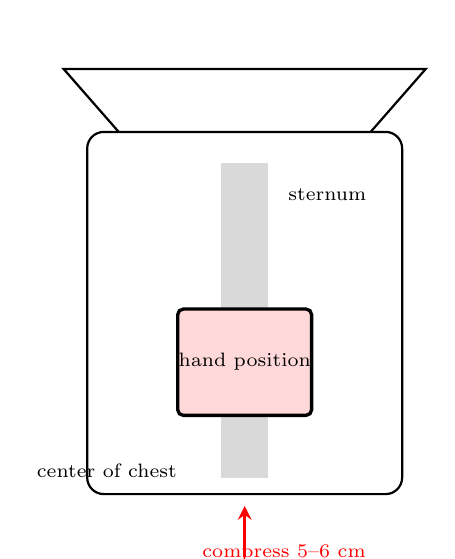
\begin{tikzpicture}[scale=1.0, >=stealth]
  \draw[thick, rounded corners=6pt] (-2.0,-2.6) rectangle (2.0,2.0);
  \draw[thick] (-1.6,2.0) -- (-2.3,2.8) -- (2.3,2.8) -- (1.6,2.0);
  \fill[gray!30] (-0.3,-2.4) rectangle (0.3,1.6);
  \node at (1.05,1.2) {\scriptsize sternum};
  \draw[very thick, fill=red!15, rounded corners=2pt] (-0.85,-1.6) rectangle (0.85,-0.25);
  \node at (0,-0.92) {\scriptsize hand position};
  \draw[->, very thick, red] (0.0,-3.4) -- (0.0,-2.75);
  \node[red] at (0.5,-3.35) {\scriptsize compress 5--6 cm};
  \node at (-1.75,-2.3) {\scriptsize center of chest};
\end{tikzpicture}
\caption{Adult CPR hand placement: heel of one hand on the center of the chest (lower half of the sternum), arms straight, pushing straight down 2--2.4 inches (5--6 cm).}
\label{fig:cpr_hands}
\end{figure}

\subsection{Rescue Breaths (If Trained and Willing)}

After 30 compressions, give 2 rescue breaths:

\begin{enumerate}[leftmargin=*]
\item Open airway using head-tilt/chin-lift maneuver: Place one hand on forehead, gently tilt head back; use second hand to lift chin point upward
\item Pinch nose shut
\item Seal your mouth over theirs and give breaths that make chest rise visibly (about 1 second each)
\item If chest does not rise, reposition head and try again
\end{enumerate}
\textbf{WARNING:} \textbf{If untrained or unwilling to give breaths, perform Hands-Only CPR}: Continuous chest compressions at 100-120 bpm without stopping for breaths. This is still effective for adults whose cardiac arrest is sudden.

\begin{center}
\begin{tabular}{@{}lll@{}}
\hline
\textbf{Group} & \textbf{Compression-Breath Ratio} & \textbf{Notes} \\
\hline
Adults (single rescuer) & 30:2 & One rescuer \\
Adults (two rescuers) & 30:2 & Standard ratio \\
Children (1 year to puberty) & 30:2 & Single rescuer \\
Children (professional/rescuer pair) & 15:2 & Two rescuers \\
Infants (<1 year) & 30:2 & Single rescuer \\
Infants (two rescuers) & 15:2 & Two rescuers \\
\hline
\end{tabular}
\end{center}

\subsection{Hands-Only CPR (Compression-Only CPR)}

If you are untrained, unsure of your skills, or unwilling to give rescue breaths, perform hands-only CPR instead of doing nothing:

\begin{enumerate}[leftmargin=*]
\item Call emergency services (or have someone else call) and place the person on their back on a firm, flat surface
\item Push hard and fast in the center of the chest: at least 2 inches (5 cm) deep, at 100--120 compressions per minute, without stopping
\item Continue until professional help arrives, an AED is ready, or the person shows signs of life
\end{enumerate}

Hands-only CPR works well for a sudden, witnessed collapse in an adult (typically a cardiac cause). Rescue breaths matter more for children, infants, and adults whose arrest follows drowning, drug overdose, or prolonged respiratory distress -- if you can give breaths, do so. If you cannot, chest compressions alone are still far better than nothing. Emergency dispatchers may also talk you through hands-only compressions.

\subsection{Two-Rescuer CPR}

If a second trained rescuer is available, coordinate to maintain high-quality compressions and effective ventilation:

\begin{itemize}[leftmargin=*]
  \item \textbf{Assign roles}: One rescuer performs chest compressions; the other gives rescue breaths (with a barrier device if available) and prepares the AED
  \item \textbf{Adult ratio}: 30 compressions to 2 breaths. For a child or infant with two rescuers, the ratio is 15:2 (see the table above)
  \item \textbf{Compression pause}: The compressor stops compressions briefly while the second rescuer gives the breaths; the second rescuer watches for visible chest rise, then signals to resume compressions immediately
  \item \textbf{Rotate every 2 minutes}: Switch roles (about every 5 cycles of 30:2) to prevent compressor fatigue and loss of compression depth. Complete the switch in less than 10 seconds -- signal on a compression count (``one, two, three...'') so the fresh rescuer takes over without a long pause
  \item \textbf{AED}: The second rescuer attaches and operates the AED, keeping everyone clear during rhythm analysis and shock delivery
  \item \textbf{Infants}: Two-rescuer infant CPR uses the two-thumb encircling technique (thumbs on the sternum, fingers encircling the chest) so one rescuer can compress while the other ventilates
\end{itemize}

\subsection{Barrier Devices (Pocket Masks and Face Shields)}

Barrier devices reduce the risk of disease transmission during rescue breathing. Use one whenever available:

\begin{itemize}[leftmargin=*]
  \item \textbf{Pocket mask}: Place the mask over the person's mouth and nose (narrow end over the bridge of the nose). Tilt the head back under the mask, seal the mask against the face with both thumbs on the sides, and breathe through the one-way valve while lifting the jaw into the mask. Watch for visible chest rise
  \item \textbf{Face shield}: Lay the shield over the face with the opening over the mouth. Seal it with your hands and breathe through the central opening while maintaining the seal
  \item With two rescuers, one rescuer can maintain the mask seal (using the head-tilt and jaw-lift) while the other compresses, allowing ventilation to be delivered in rhythm without breaking hand position
  \item If no barrier device is available, perform rescue breaths without one, or fall back to hands-only CPR -- doing something is always better than nothing
\end{itemize}

\subsection{High-Quality CPR Essentials}

The survival benefit of CPR depends on how well it is performed. Focus on these quality measures:

\begin{itemize}[leftmargin=*]
  \item \textbf{Minimize interruptions}: Keep pauses in compressions under 10 seconds. Stop only for rhythm analysis, shock delivery, or role rotation
  \item \textbf{Maximize the compression fraction}: Aim to be compressing the chest more than 80\% of the total time
  \item \textbf{Full recoil}: Allow the chest to completely expand between compressions; do not lean on the chest
  \item \textbf{Correct depth and rate}: Adults 2--2.4 inches (5--6 cm) at 100--120 per minute; allow no drift from fatigue -- this is why rescuers rotate
  \item \textbf{Avoid excessive ventilation}: Give each breath over about 1 second with just enough volume to make the chest rise visibly; too much or too fast ventilation reduces blood return to the heart
  \item \textbf{Coordinate with the AED}: When the AED is analyzing or delivering a shock, compressions pause; the moment it finishes, resume compressions immediately without delay
\end{itemize}

\section{Pediatric CPR (Infants and Children)}

\subsection{Infant CPR (Under 1 Year Old)}

\subsubsection{Technique Differences}

\begin{itemize}[leftmargin=*]
  \item Use two fingers (middle and ring) on the center of the chest just below the nipple line
  \item Or use two-thumb encircling technique (for two rescuers): thumbs side-by-side on lower third of sternum, fingers around back supporting the chest
  \item Compression depth: about 1.5 inches (4 cm) -- one-third the depth of the chest
  \item Rate: 100-120 bpm
  \item Rescue breaths: Cover both mouth AND nose when giving breaths (small mouth-to-mouth seal)
\end{itemize}

\subsection{Child CPR (1 Year to Puberty)}

\begin{itemize}[leftmargin=*]
  \item Use one or two hands depending on child size (one hand may suffice for smaller children)
  \item Compression depth: about 2 inches (5 cm)
  \item Rate: 100-120 bpm
  \item Follow adult compression technique otherwise
\end{itemize}

\textbf{WARNING:} \textbf{Important: Pediatric cardiac arrest is often respiratory in origin. Ensure proper airway positioning and adequate ventilation are emphasized in addition to compressions.}

\subsection{Moving a Child or Infant During CPR}

Begin CPR where you find the child or infant if the scene is safe. Move them ONLY if:

\begin{itemize}[leftmargin=*]
  \item The current location is unsafe (fire, electrical hazard, water, traffic, violence)
  \item The surface is too soft to allow effective compressions (e.g., a sagging mattress) and a firm surface is immediately available
  \item You are already moving to reach help or a family member
\end{itemize}

How to move: for an infant, support the head and neck with one hand and cradle the body with your forearm; for a child, carry them in your arms supporting the head. Minimize movement and avoid bending or twisting the neck. Once on a firm surface, resume CPR immediately. Do NOT delay compressions to reposition a child who is already on a firm, safe surface.

\section{Automated External Defibrillator (AED)}

An AED is a portable device that analyzes heart rhythm and delivers shocks if needed. Early defibrillation dramatically improves survival from ventricular fibrillation/pulseless ventricular tachycardia.

\subsection{AED Usage Steps}

\begin{enumerate}[leftmargin=*]
\item Turn on the AED (follow voice prompts)
\item Expose the person's bare chest and wipe dry if wet
\item Attach electrode pads as shown in diagram on package: upper right chest (below collarbone) and lower left side (below armpit)
\item Ensure nobody touches the person while the AED analyzes the rhythm
\item Follow AED prompts: If shock advised, ensure everyone is clear and press the shock button. If no shock advised, resume CPR immediately
\end{enumerate}
\begin{figure}[h]
\centering
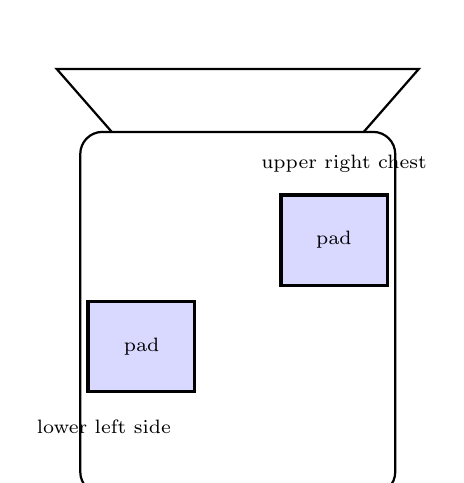
\begin{tikzpicture}[scale=1.0, >=stealth]
  \draw[thick, rounded corners=8pt] (-2.0,-2.6) rectangle (2.0,2.0);
  \draw[thick] (-1.6,2.0) -- (-2.3,2.8) -- (2.3,2.8) -- (1.6,2.0);
  \draw[very thick, fill=blue!15] (0.55,1.2) rectangle (1.9,0.05);
  \node at (1.22,0.63) {\scriptsize pad};
  \draw[very thick, fill=blue!15] (-1.9,-0.15) rectangle (-0.55,-1.3);
  \node at (-1.22,-0.73) {\scriptsize pad};
  \node at (1.35,1.6) {\scriptsize upper right chest};
  \node at (-1.7,-1.75) {\scriptsize lower left side};
\end{tikzpicture}
\caption{AED electrode pad placement: one pad on the upper right chest below the collarbone, the other on the lower left side below the armpit.}
\label{fig:aed_pads}
\end{figure}

\quicknote{\textbf{Defibrillation Priority}: For a witnessed collapse where someone can grab an AED immediately, use the AED as soon as possible, even before beginning extensive CPR. Unwitnessed collapse starts with CPR first.}

\textbf{WARNING:} \textbf{Pacemakers}: If you see a hard lump under the skin on the chest (pacemaker or ICD), avoid placing the electrode pad directly over it. Place the pad at least 1 inch away.

\quicknote{\textbf{Children}: For children under 8 years or under 25 kg (55 lbs), use pediatric pads or a dose-attenuating device if available. If only adult pads are available, use them -- delivering a shock is preferable to no shock. For children under 1 year, an AED may be used with pediatric pads or a dose-attenuator if available.}

\subsubsection{AED Use in Infants}
For infants under 1 year old:
\begin{itemize}
  \item Preferred: Use a pediatric AED with child-sized pads or a dose-attenuator that reduces the shock energy
  \item If pediatric AED is not available: Use a standard AED with adult pads -- do not withhold defibrillation
  \item Pad placement: anterior--posterior (one pad on center of chest, one on center of back) is preferred for infants if using adult pads, to prevent pads from touching
  \item If pads would touch on the front and back, use the anterior--posterior placement rather than risking contact
\end{itemize}
\textbf{WARNING}: Never use a pediatric dose-attenuator with an AED designed only for adult use, and never use adult pads on an infant if pediatric pads are available -- the shock energy may be excessive.

\subsection{Special Situations and Pad Placement}

\begin{itemize}[leftmargin=*]
  \item \textbf{Medication patches}: If a patch (e.g., nitroglycerin, nicotine, pain reliever) is on the chest where a pad will go, remove it with a gloved hand and wipe the skin dry before attaching the pad -- patches can conduct electricity and cause burns during shock delivery
  \item \textbf{Wet chest}: Dry the chest thoroughly before attaching pads; pads will not stick to wet or sweaty skin
  \item \textbf{Dense chest hair}: If the pads do not stick well, shave the area quickly with the razor included in the AED kit, or press the pads firmly through the hair. Do not delay shocks for extensive shaving
  \item \textbf{Jewelry and piercings}: Leave jewelry and piercings in place unless they sit directly under a pad; move the pad slightly. Do not waste time removing jewelry
  \item \textbf{Pacemaker or ICD}: If you see or feel a hard lump under the skin on the chest, place the pad at least 1 inch away from it (see the warning above)
  \item \textbf{Water}: Do not use an AED on a person lying in water or a puddle -- move them to a dry surface before attaching pads (and before CPR)
  \item \textbf{Alternate pad positions}: If standard pad placement is not possible (e.g., an implanted device or injury in the way), use the anterior--posterior position: one pad on the front of the chest and the other on the back between the shoulder blades
\end{itemize}

\section{Airway Management in First Aid}

Maintaining a patent airway is essential in any unconscious patient.

\subsection{Head-Tilt/Chin-Lift Maneuver}

Used to open the airway in an unresponsive person without suspected spinal injury.

\begin{enumerate}[leftmargin=*]
\item Place hand on forehead and apply firm, backward pressure
\item Use fingertips under bony part of lower jaw and lift forward
\item This tilts the head back and lifts tongue away from posterior pharyngeal wall
\end{enumerate}
\textbf{WARNING:} \textbf{Suspected Spinal Injury}: Use the Jaw-Thrust Maneuver instead: place hands on either side of head, grasp angles of mandible, and lift forward WITHOUT tilting the head. Maintain manual in-line stabilization of the neck throughout.

\subsection{Recovery Position}

See Section~\ref{sec:recovery_position} in Chapter~\ref{ch:basic_principles} for detailed instructions. Essential for maintaining airway patency in breathing but unconscious persons.

\section{Choking Management}

Conscious choking requires immediate intervention to relieve airway obstruction.

\subsection{Conscious Adult or Child Over 1 Year}

\begin{enumerate}[leftmargin=*]
  \item Ask ``Are you choking?'' If yes, encourage coughing if they can still cough, speak, or breathe (this indicates partial obstruction)
  \item If they cannot cough, speak, or breathe (severe obstruction), begin Heimlich maneuver (abdominal thrusts)
  \item Stand behind the person, wrap arms around their waist, make fist with one hand, grasp it with other, place thumb side just above navel
  \item Give quick, upward and inward thrusts until object is expelled or person becomes unconscious
\end{enumerate}
\textbf{WARNING:} \textbf{Do not perform abdominal thrusts on pregnant women or obese persons. Use chest thrusts instead: Place heel of hand on center of breastbone, give quick inward and upward thrusts.}

\subsection{Conscious Infant (Under 1 Year)}

Abdominal thrusts are dangerous for infants. Use back blows combined with chest thrusts:

\begin{enumerate}[leftmargin=*]
\item Support infant face-down along forearm, head lower than chest, support head with hand
\end{enumerate}
\begin{figure}[h]
\centering
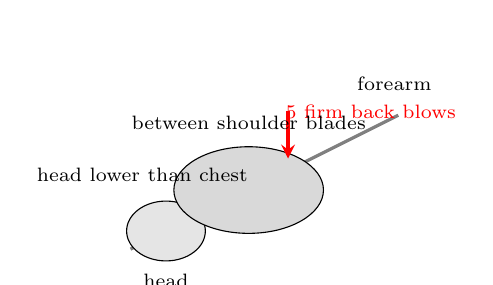
\begin{tikzpicture}[scale=1.0, >=stealth]
  \draw[very thick, gray] (0,0) -- (3.4,1.7);
  \node at (3.35,2.1) {\scriptsize forearm};
  \draw[fill=black!10] (0.45,0.23) ellipse (0.5 and 0.38);
  \draw[fill=black!15] (1.5,0.75) ellipse (0.95 and 0.55);
  \node at (0.45,-0.4) {\scriptsize head};
  \node at (0.15,0.95) {\scriptsize head lower than chest};
  \draw[->, very thick, red] (2.0,1.75) -- (2.0,1.15);
  \node[red] at (3.05,1.75) {\scriptsize 5 firm back blows};
  \node at (1.5,1.6) {\scriptsize between shoulder blades};
\end{tikzpicture}
\caption{Infant choking: hold the infant face-down along your forearm with the head supported and lower than the chest, then give 5 firm back blows between the shoulder blades.}
\label{fig:infant_backblows}
\end{figure}

\begin{enumerate}[leftmargin=*]
\item Give up to 5 firm back blows between shoulder blades with heel of hand
\item If object not expelled, turn infant face-up along forearm, support head, keep head lower than chest
\item Give up to 5 chest thrusts using two fingers on lower third of sternum (same position as compressions), pressing down about 1.5 inches
\item Alternate 5 back blows and 5 chest thrusts until object expelled or infant becomes unconscious
\end{enumerate}
\subsection{Unconscious Person (Adult, Child, or Infant)}

Lower the person carefully to the ground and begin CPR starting with chest compressions. Before rescue breaths, check the mouth for visible object; if seen, remove with finger sweep. Attempt breath; if unsuccessful, reposition head and try again. Continue CPR cycle until help arrives or object dislodges.

\medskip\noindent\textbf{CPR Quick Reference Summary.}
\begin{center}
\begin{tabularx}{\textwidth}{@{}>{\raggedright\arraybackslash}l>{\raggedright\arraybackslash}X>{\raggedright\arraybackslash}X@{}}
\hline
\textbf{Parameter} & \textbf{Adult} & \textbf{Infant/Child} \\
\hline
Compression Depth & 2-2.4 inches (5-6 cm) & 1.5-2 inches (4-5 cm) \\
Compression Rate & 100-120 bpm & 100-120 bpm \\
Compression Technique & Both hands stacked (heel on heel) & Two fingers (infant) / One or two hands (child) \\
Ratio (Single Rescuer) & 30:2 & 30:2 \\
Ratio (Two Rescuers Children) & 30:2 & 15:2 \\
\hline
\end{tabularx}
\end{center}

\section{Special Considerations}

\subsection{Dental Work and Dentures}

If dentures are loose during rescue breaths, remove them to get a better seal. If tightly fitted, leave in place as they may help form the seal.

\subsection{Person in Water (Water Rescue CPR)}

For drowning victims, provide rescue breathing promptly after removing from water. Perform 5 initial cycles of CPR (about 2 minutes) before calling for help if alone and witnessed. Prioritize rapid extrication and ventilation.

\subsection{Suspected Stroke}

Recognize FAST: Face drooping, Arm weakness, Speech difficulty, Time to call emergency services. While waiting, keep person comfortable, do not give food or drink, monitor breathing, and be prepared to initiate CPR if they become unresponsive.

\section{When Professional Help Arrives}

\begin{itemize}[leftmargin=*]
  \item Report what you observed (collapse time, CPR started/stopped times, AED usage/shocks delivered)
  \item Describe any interventions you performed
  \item Inform about medication known history if available
  \item Do not stop CPR unless directed by medical personnel or the person shows signs of life (movement, normal breathing, responsiveness)
\end{itemize}

\section{Review Questions}

\begin{enumerate}[leftmargin=*]
\item How do you locate the correct hand position for adult chest compressions, and what is the recommended depth and rate?
\item What is the correct compression-to-ventilation ratio for a single rescuer performing CPR on an adult? On an infant?
\item Why is the head-tilt/chin-lift not used when a spinal injury is suspected, and what replaces it?
\item When should a child or infant be moved (not left where they are) during CPR, and how?
\item What does a shockable rhythm mean for AED use, and what should you do if the AED does not advise a shock?
\item How does choking relief differ between an infant and an adult?
\end{enumerate}
\section{Skill Practice: CPR and Airway}

\begin{enumerate}[leftmargin=*]
\item Check scene safety and demonstrate the responsive and unresponsive checks
\item Call for help and ask for an AED (simulate)
\item Demonstrate head-tilt/chin-lift and open the airway
\item Practice 5 cycles of 30:2 chest compressions and rescue breaths on a manikin or model (check depth and rate with a partner or timer)
\item Demonstrate the jaw-thrust technique for a suspected spinal injury
\item Show AED pad placement from memory on a volunteer or diagram
\item Practice the Heimlich maneuver on a partner using appropriate force
\item Practice infant back blows and chest thrusts on a doll or rolled towel
\end{enumerate}
\index{cardiopulmonary resuscitation (CPR)}
\index{chest compressions}
\index{rescue breaths}
\index{automated external defibrillator (AED)}
\index{adult CPR}
\index{pediatric CPR}
\index{infant CPR}
\index{Heimlich maneuver}
\index{choking relief}
\index{airway management}
\index{jaw-thrust maneuver}
\index{head-tilt/chin-lift}
\index{stroke recognition}
\index{drowning response}
\index{defibrillation}
\index{hands-only CPR}
\index{compression-only CPR}
\index{two-rescuer CPR}
\index{pocket mask}
\index{face shield}
\index{barrier devices}
\index{high-quality CPR}
\chapter{Medical Emergencies}\label{ch:medical}

\section{Heart Attack (Myocardial Infarction)}

A heart attack occurs when blood flow to part of the heart muscle is blocked, often by a blood clot in a coronary artery. Prompt recognition and response are critical for survival and reducing heart damage.

\subsection{Signs and Symptoms}

\begin{itemize}[leftmargin=*]
  \item Chest pain or discomfort: Pressure, squeezing, fullness, or pain in center or left side of chest lasting more than a few minutes or coming and going
  \item Pain radiating to arm (especially left arm), back, neck, jaw, or stomach
  \item Shortness of breath with or without chest discomfort
  \item Breaking out in a cold sweat
  \item Nausea or vomiting
  \item Lightheadedness or sudden dizziness
  \item Unusual fatigue (particularly in women)
\end{itemize}

\noindent\textbf{\textcolor{red}{WARNING}}: \textit{Symptoms vary by gender}: Women are more likely to experience shortness of breath, nausea/vomiting, and back/jaw pain. Both men and women can experience unusual fatigue. Older adults and people with diabetes may have milder symptoms or no chest pain at all.

\subsection{Immediate Actions}

\begin{enumerate}[leftmargin=*]
\item Have the person stop all activity and rest comfortably -- sitting or semi-reclining position is usually best
\item Call emergency services immediately (dial 112 or 108 in India). Do not drive the person yourself unless absolutely necessary
\item If prescribed nitroglycerin is available and the person is conscious, assist them in taking it as directed (usually one tablet under the tongue every 5 minutes up to three doses)
\item Ask if they carry aspirin; if yes and they are not allergic (and have not been advised by their doctor against it), chew one adult aspirin (325 mg) or four low-dose aspirins (81 mg each) -- chewing absorbs faster \cite{aha_arc_2024}
\end{enumerate}
\noindent\textbf{\textcolor{red}{NOTE}}: \textit{ASPIRIN WARNING}: Only give aspirin if the person has NO allergy to it, has NOT been advised by a doctor against taking it, and you are reasonably sure they are having a heart attack (not a bleeding condition like stroke). Do NOT give aspirin to children or teenagers.

\begin{enumerate}[leftmargin=*]
\item Monitor breathing continuously. If they become unresponsive and not breathing normally, begin CPR immediately
\end{enumerate}
\noindent\textbf{\textcolor{red}{DO NOT}}: Give anything by mouth (food, drink, other medications) unless specifically prescribed; let the person walk around to ``walk off'' the discomfort; assume it's just indigestion without medical evaluation; drive the person to the hospital yourself.

\section{Stroke}

A stroke occurs when blood supply to part of the brain is interrupted or reduced, preventing brain tissue from getting oxygen and nutrients. Brain cells begin to die within minutes.

\subsection{Recognition -- The FAST Mnemonic}

\begin{center}
\begin{tabular}{@{}ll@{}}
\textbf{F} -- Face & Ask the person to smile. Is one side of the face drooping? \\
\textbf{A -- Arm} & Ask the person to raise both arms. Does one arm drift downward? \\
\textbf{S -- Speech} & Ask the person to repeat a simple phrase. Is speech slurred or strange? \\
\textbf{T -- Time} & If any of these signs are present, call emergency services immediately! \\
\end{tabular}
\end{center}

Additional stroke signs include:

\begin{itemize}[leftmargin=*]
  \item Sudden confusion or trouble understanding speech
  \item Sudden trouble seeing in one or both eyes
  \item Sudden severe headache with no known cause ("worst headache of my life")
  \item Sudden trouble walking, dizziness, loss of balance or coordination
\end{itemize}

\subsection{Management}

\begin{enumerate}[leftmargin=*]
\item Call emergency services immediately -- time is brain
\item Note the exact time when symptoms first appeared. This is critical information for medical treatment decisions
\item Keep the person comfortable and calm. Loosen tight clothing
\item Do NOT give food, drink, or medication (risk of aspiration if consciousness changes)
\item If the person becomes unconscious but is breathing, place them in the recovery position
\end{enumerate}
\noindent\textbf{\textcolor{red}{WARNING}}: Even if symptoms resolve quickly, this could be a transient ischemic attack (TIA or "mini-stroke"), which requires immediate medical evaluation as it often precedes a full stroke. Always seek emergency care for suspected stroke.

\section{Seizures (Epileptic Seizure)}

A seizure is a disturbance in normal electrical activity in the brain that can cause changes in behavior, movements, feelings, or levels of consciousness.

\subsection{Types of Seizures}

\begin{description}[leftmargin=!]
  \item[Generalized Tonic-Clonic (Grand Mal)] Loss of consciousness, body stiffens (tonic phase), followed by rhythmic jerking (clonic phase)
  \item[Absence (Petit Mal)] Brief staring spells (seconds), mostly in children
  \item[Partial/Focal] May involve localized jerking, altered awareness, or sensory changes without full loss of consciousness
\end{description}

\subsection{During a Seizure}

\begin{enumerate}[leftmargin=*]
\item Stay calm and time the seizure
\item Protect the person from injury by moving objects away and placing something soft under their head
\item Turn the person onto their side if possible to help maintain airway and allow fluids to drain
\item Loosen tight clothing around the neck
\end{enumerate}
\noindent\textbf{\textcolor{red}{NEVER}}: Put anything in the person's mouth (can cause broken teeth or jaw injury); try to force the person awake during the seizure; offer water or pills until fully alert and able to swallow safely.

\subsection{After the Seizure (Post-Ictal Phase)}

\begin{itemize}[leftmargin=*]
  \item Stay with the person until they are fully awake and oriented
  \item Offer reassurance and explain what happened
  \item Allow them to rest; some feel tired or confused afterward
  \item Do not force them to eat or drink until fully conscious and able to swallow safely
  \item Check for injuries that occurred during the seizure
\end{itemize}

\noindent\textbf{\textcolor{red}{When to Call Emergency Services}}: First-time seizure; seizure lasts longer than 5 minutes; second seizure occurs before the person recovers; difficulty breathing after seizure; person is injured; person does not regain consciousness; person has diabetes or is pregnant; seizure occurs in water.

\noindent\textbf{\textcolor{green}{PEARL}}: \textit{Seizure First Aid Summary}
\begin{enumerate}
  \item Protect from injury (move things away, pad head)
  \item Turn person onto their side
  \item Time the seizure
  \item Do not put anything in the mouth
  \item Do not restrain
  \item Stay with person until fully recovered
\end{enumerate}

\section{Diabetic Emergencies}

Both high blood sugar (hyperglycemia) and low blood sugar (hypoglycemia) are potential emergencies in people with diabetes.

\subsection{Hypoglycemia (Low Blood Sugar)}

Occurs when blood glucose falls below normal levels. Common causes: missed meals, excessive insulin, increased physical activity.

\subsubsection{Symptoms}

\begin{itemize}[leftmargin=*]
  \item Shakiness, sweating, trembling
  \item Rapid heartbeat or palpitations
  \item Hunger
  \item Dizziness, lightheadedness
  \item Confusion, irritability, anxiety
  \item Blurred vision
  \item Weakness, fatigue
  \item In severe cases: seizures, loss of consciousness
\end{itemize}

\subsubsection{Management (Conscious Person)}

\begin{enumerate}[leftmargin=*]
\item Administer fast-acting carbohydrates: 15 grams of simple sugar (glucose tablets, juice, regular soda, honey)
\item Wait 15 minutes and check blood sugar if possible
\item Repeat if still low
\item Once blood sugar is stable, provide a snack or meal containing protein and complex carbohydrates
\end{enumerate}
\noindent\textbf{\textcolor{red}{UNCONSCIOUS PERSON}}: Do NOT attempt to give anything by mouth (choking hazard). Apply glucose gel/tube inside the cheek if available and trained to use. Call emergency services immediately. Administer glucagon injection if prescribed and trained. Do NOT give food or drink until fully conscious and able to swallow.

\subsection{Hyperglycemia (High Blood Sugar)}

Occurs when there is too much glucose in the blood. Can progress to diabetic ketoacidosis (DKA) in type 1 diabetes or hyperosmolar hyperglycemic state (HHS) in type 2 diabetes.

\subsubsection{Symptoms}

\begin{itemize}[leftmargin=*]
  \item Extreme thirst
  \item Frequent urination
  \item Blurred vision
  \item Fatigue, weakness
  \item Headache
  \item Dry mouth and skin
  \item Fruity-smelling breath (DKA warning sign)
\end{itemize}

\subsubsection{Management}

\begin{enumerate}[leftmargin=*]
  \item Check blood sugar if possible
  \item Help the person take prescribed insulin only if they are conscious, alert, and able to swallow safely
  \item Encourage drinking water (if conscious, alert, and able to swallow safely — do NOT force fluids)
  \item Seek medical attention immediately if blood sugar remains extremely high (>300 mg/dL in adults), or if there are signs of ketones, fruity breath, confusion, or difficulty breathing
  \item If the person is unconscious, confused, or unable to swallow safely, DO NOT give food, drink, or insulin — seek emergency medical help immediately
\end{enumerate}
\noindent\textbf{\textcolor{red}{RECOGNIZING DKA}}: Look for rapid deep breathing (Kussmaul breathing), abdominal pain, nausea/vomiting, and fruity breath odor. This is a life-threatening emergency requiring immediate hospital care.


\section{Bee and Insect Stings}

Bees, wasps, hornets, and ants can sting, causing pain, redness, and swelling at the sting site. Most stings produce only local symptoms, but some people may develop a severe allergic reaction (anaphylaxis).

\subsection{Local Reaction (Most Common)}

These symptoms affect only the area around the sting and typically improve within hours to days.

\begin{itemize}[leftmargin=*]
  \item Immediate sharp pain or burning at the site
  \item Red welt at the sting location
  \item Localized swelling and itching
\end{itemize}

\subsubsection{Management}

\begin{enumerate}[leftmargin=*]
  \item Wash the area with soap and water to reduce infection risk
  \item Remove the stinger if present by scraping it sideways with a fingernail or credit card — DO NOT squeeze or pinch (this can inject more venom)
  \item Apply a cold pack or ice wrapped in cloth for 10-15 minutes at a time to reduce pain and swelling
  \item Elevate the affected limb if possible
  \item Use over-the-counter pain relievers (acetaminophen or ibuprofen) for pain
  \item Apply calamine lotion or hydrocortisone cream to reduce itching
  \item Take an oral antihistamine (e.g., diphenhydramine/Benadryl) if available and appropriate for the person's age and health
  \item Monitor for signs of allergic reaction that spread beyond the sting site (see below)
\end{enumerate}
\noindent\textbf{Note}: A large local reaction (increasing redness and swelling over several days, up to 4 inches in diameter) is different from an allergic reaction and usually resolves on its own. If swelling continues to worsen after 48 hours or shows signs of infection (pus, increasing warmth, red streaks), seek medical care.

\subsection{Systemic Allergic Reaction (Anaphylaxis)}

Some people experience a whole-body allergic reaction that can become life-threatening within minutes. This requires immediate action even if the person has never had a severe reaction before.

\textbf{Symptoms may include}: Skin hives or swelling away from the sting site; difficulty breathing, wheezing, or throat tightness; nausea, vomiting, or dizziness; rapid heartbeat; feeling of impending doom.

\textbf{If any systemic symptoms develop, treat as anaphylaxis immediately}: See the Anaphylaxis section below for emergency management including epinephrine administration and calling emergency services.


\section{Anaphylaxis (Severe Allergic Reaction)}

Anaphylaxis is a life-threatening systemic allergic reaction that can occur rapidly after exposure to an allergen. Common triggers: foods (peanuts, tree nuts, shellfish, eggs, milk), insect stings, medications, latex.

\subsection{Symptoms}

\begin{itemize}[leftmargin=*]
  \item Skin: Hives, itching, flushing, swelling (especially lips, tongue, face, throat)
  \item Respiratory: Wheezing, difficulty breathing, stridor (high-pitched sound when inhaling), hoarseness, coughing
  \item Cardiovascular: Rapid or weak pulse, pale/blue skin, dizziness, fainting, low blood pressure
  \item Gastrointestinal: Nausea, vomiting, abdominal cramps, diarrhea
  \item Others: Sense of impending doom, anxiety
\end{itemize}

\noindent\textbf{\textcolor{red}{EMERGENCY}}: Anaphylaxis can progress rapidly within minutes. Delay in epinephrine administration increases risk of death.

\subsection{Management}

\begin{enumerate}[leftmargin=*]
\item Identify and remove the allergen if possible (e.g., sting stinger scraped out sideways with fingernail)
\item Assist the person in using their prescribed epinephrine auto-injector (EpiPen, Auvi-Q, etc.) if available
\item Call emergency services immediately
\item Lie the person flat with legs elevated (unless breathing difficulty makes this uncomfortable, then allow semi-upright position)
\item Monitor breathing and circulation; prepare to perform CPR if needed
\item A second dose of epinephrine may be given after 5-15 minutes if symptoms persist or worsen and another auto-injector is available
\end{enumerate}
\noindent\textbf{\textcolor{green}{NOTE}}: \textit{Epinephrine Administration}: Inject into the outer thigh muscle through clothing if necessary. Hold in place for several seconds to ensure full dose delivery. Massage the injection site gently afterwards.

\noindent\textbf{\textcolor{green}{PEARL}}: \textit{Allergy Action Plan Reminder}

Always ask individuals with known severe allergies if they carry an epinephrine auto-injector and how you should assist if needed. Many people wear medical identification indicating their allergies and emergency instructions.

\section{Asthma Attack}

An asthma attack involves narrowing of the airways due to inflammation and muscle constriction, causing breathing difficulties.

\subsection{Symptoms}

\begin{itemize}[leftmargin=*]
  \item Difficulty breathing or shortness of breath
  \item Wheezing (whistling sound when breathing)
  \item Persistent coughing
  \item Chest tightness or pain
  \item Anxiety, panic from difficulty breathing
  \item Pale, sweaty, or bluish skin (severe attack)
\end{itemize}

\subsection{Management}

\begin{enumerate}[leftmargin=*]
\item Help the person remain calm and sit upright (this helps air movement better than lying down)
\item Assist in using their rescue inhaler (usually albuterol/salbutamol): shake, prime if new, take one puff and wait one minute, repeat as prescribed (typically 1-2 puffs every 4-6 hours as needed)
\item Call emergency services if: no improvement after 2-3 puffs over 10 minutes; speaking in words instead of sentences; lips/fingernails turning blue; feeling increasingly worse; never been diagnosed before; symptoms recur after initial improvement
\end{enumerate}
\noindent\textbf{\textcolor{red}{WARNING}}: Never give anyone else's asthma inhaler unless specifically authorized. Do not slap their back during an attack (this can make it worse).

\section{Other Medical Emergencies}

\subsection{Unexplained Loss of Consciousness (Syncope/Passing Out)}

Syncope is a brief, temporary loss of consciousness caused by a temporary drop in blood flow to the brain. Most causes are benign, but some are dangerous.

\subsubsection{Common Causes}

\begin{itemize}[leftmargin=*]
  \item \textbf{Vasovagal (simple) fainting}: triggered by pain, fear, anxiety, the sight of blood, or standing for long periods
  \item \textbf{Orthostatic (postural) hypotension}: a sudden drop in blood pressure when standing up quickly, especially in older adults or after dehydration
  \item \textbf{Dehydration or low blood sugar}
  \item \textbf{Dangerous causes}: heart rhythm problems, heart attack, internal bleeding, or stroke -- these require immediate medical care
\end{itemize}

\subsubsection{Immediate Management}

\begin{enumerate}[leftmargin=*]
  \item Lay the person flat on their back
  \item Raising the legs above heart level may be considered ONLY if the cause is non-traumatic (e.g., simple fainting) and it does not cause pain or worsen symptoms
  \item Loosen tight clothing
  \item Check breathing and pulse; if not breathing normally, begin CPR
  \item If conscious and recovering, allow them to rest and sit up gradually -- do not let them stand quickly
  \item Offer small sips of water once fully alert (if the cause may be dehydration) or a source of quick sugar if low blood sugar is suspected
  \item Seek medical evaluation for any unexplained syncope
\end{enumerate}
\subsubsection{Red Flags -- Call Emergency Services}

\begin{itemize}[leftmargin=*]
  \item Fainting during or right after exertion, exercise, or physical activity
  \item Fainting without any warning signs (no nausea, sweating, or lightheadedness beforehand)
  \item Fainting with palpitations (racing or fluttering heartbeat) or chest pain
  \item The person does not recover quickly or is confused after waking
  \item Repeated episodes, fainting during pregnancy, or any known heart condition
  \item The person is injured from the fall, or is taking blood-thinning medication
\end{itemize}

\quicknote{The person who wakes up quickly and feels well after a simple fainting spell (stress, heat, or standing too long) is usually not in danger. Fainting during exercise, without warning, or with palpitations or chest pain suggests a possible cardiac cause and must be evaluated by a doctor.}

\subsection{Blood Pressure Emergencies}

\subsubsection{High Blood Pressure Emergency (Hypertensive Emergency)}

Most people with high blood pressure (hypertension) feel no symptoms. Rarely, very high blood pressure causes acute damage to organs (brain, heart, eyes, kidneys) -- this is a hypertensive emergency and requires urgent hospital care.

\textbf{Recognize -- seek emergency care if these occur together or worsen:}
\begin{itemize}[leftmargin=*]
  \item A very severe headache, different from the person's usual headaches
  \item Blurred or double vision, or visual disturbances
  \item Chest pain or shortness of breath
  \item Confusion, personality changes, or difficulty speaking
  \item Nausea and vomiting, or weakness/numbness on one side of the body
  \item Nosebleeds that will not stop
\end{itemize}

\textbf{Management:}
\begin{enumerate}[leftmargin=*]
  \item Call emergency services immediately
  \item Have the person sit or lie down comfortably and remain calm
  \item Loosen tight clothing
  \item Do NOT give any blood pressure medication that is not theirs, and do not take extra doses of their own medication without medical direction
  \item Monitor responsiveness and breathing; be ready to begin CPR
  \item Do NOT ignore these symptoms as "just a headache" -- without treatment, a hypertensive emergency can cause stroke, heart attack, or organ damage
\end{enumerate}
\subsubsection{Low Blood Pressure (Hypotension)}

Low blood pressure (hypotension) is only an emergency when it causes symptoms, most commonly lightheadedness or fainting when standing up. It can follow dehydration, bleeding, infection, or allergic reactions.

\begin{itemize}[leftmargin=*]
  \item If the person feels faint: lay them flat, raise the legs only for non-traumatic causes, and let them recover gradually
  \item Give small sips of water if dehydration is suspected and the person is alert and able to swallow
  \item Seek emergency care if low blood pressure is accompanied by confusion, chest pain, shortness of breath, black/tarry stools, vomiting blood, or signs of severe allergic reaction
  \item A one-time reading on a home monitor with no symptoms is rarely an emergency -- but any unexplained, repeated, or severe readings should be discussed with a doctor
\end{itemize}

\subsection{Heat Illness}

See Chapter~\ref{ch:environmental} for detailed management of heat exhaustion and heat stroke.

\subsection{Poisoning}

Poisoning can occur through ingestion, inhalation, skin contact, or injection. Signs vary widely but may include nausea, vomiting, confusion, drowsiness, seizures, breathing difficulty, and burns around the mouth.

\textbf{General Principles:}

\begin{itemize}
  \item Remove the substance from the person if safe (brush off powder, flush chemicals with water) -- protect yourself with gloves or a barrier
  \item Do NOT induce vomiting unless instructed by poison control or medical professionals
  \item Call poison control center or emergency services immediately
  \item Keep the product container/poison source and any remains for medical personnel to identify
  \item Note the substance, approximate amount, and time of exposure
  \item If the person vomits, position them on their side to protect the airway
  \item Monitor breathing and level of consciousness; be ready to begin CPR
\end{itemize}

\textbf{Poison Control Numbers:}

\begin{center}
\small
\begin{tabularx}{\textwidth}{@{}>{\raggedright\arraybackslash}lX>{\raggedright\arraybackslash}r@{}}
\hline
\textbf{Location} & \textbf{Contact} & \textbf{Notes} \\
\hline
India (AIIMS NPIC) & 011-26589391, 011-26593677 & 24-hour helpline, New Delhi \\
India (State Poison Cells) & Check local health department & Regional centers in major cities \\
United States & 1-800-222-1222 & 24/7, American Association of Poison Control Centers \\
United Kingdom & 111 or 999 & NHS non-emergency or emergency \\
Australia & 13 11 26 & Poisons Information Centre \\
European Union & Local poison control center & Varies by country \\
\hline
\end{tabularx}
\end{center}

\textbf{Note}: Program the nearest poison control number into your phone before you need it. In India, the National Poisons Information Centre at AIIMS, New Delhi, is the primary reference for toxicological emergencies and can guide treatment decisions for common household poisons, snake antivenom selection, and pesticide exposures.

\subsubsection{Opioid Overdose}

Opioids (heroin, fentanyl, morphine, oxycodone, and similar) slow and can stop breathing. Overdose may occur with prescription painkillers or street drugs.

\begin{itemize}[leftmargin=*]
  \item \textbf{Recognize}: extreme drowsiness or unresponsiveness, slow or absent breathing, pinpoint pupils, blue-gray lips or nails
  \item Call emergency services immediately -- opioid overdose is reversible \cite{ilcor_2025,aha_arc_2024}
  \item Administer naloxone (Narcan) if available and you are trained: one dose into the nose or muscle, repeat every 2-3 minutes if no response
  \item Begin rescue breathing or CPR if breathing is absent but a pulse is present
  \item Naloxone wears off in 30-90 minutes -- continue to monitor and keep the person with medical personnel even if they wake up
  \item Do NOT leave the person alone; a second overdose can occur as naloxone wears off
\end{itemize}

\subsubsection{Alcohol Poisoning}

Alcohol can suppress the brain's control of breathing, heart rate, and gag reflex. Severe intoxication can be fatal.

\begin{itemize}[leftmargin=*]
  \item \textbf{Recognize}: confusion or stupor, vomiting, cold/clammy skin, slow or irregular breathing, low body temperature, seizures, unresponsiveness
  \item Call emergency services for anyone who is unconscious, has been vomiting repeatedly, or cannot be roused
  \item Turn an unconscious or vomiting person onto their side to prevent choking
  \item Do NOT give food, coffee, or more alcohol to "sober them up"
  \item Do NOT leave an intoxicated person to "sleep it off" -- their breathing can stop
\end{itemize}

\subsubsection{Carbon Monoxide (CO) Poisoning}

CO is an odorless, colorless gas from fires, vehicle exhaust, generators, and faulty heaters. It displaces oxygen from the blood.

\begin{itemize}[leftmargin=*]
  \item \textbf{Recognize}: headache, dizziness, nausea, weakness, confusion, chest pain, and cherry-red lips in severe cases (rare); multiple people becoming ill in the same building or vehicle is a clue
  \item Move the person to fresh air immediately -- do not enter an enclosed space without ventilation unless you can stay safe
  \item Call emergency services; anyone exposed needs medical evaluation even if they feel better in fresh air
  \item Do NOT assume recovery is complete -- CO poisoning requires oxygen therapy at a hospital
\end{itemize}

\noindent\textbf{\textcolor{red}{PREVENTION}}: Install carbon monoxide detectors near sleeping areas and test them monthly. Never run generators, cars, or heaters indoors or in attached garages.


\subsection{Caustic or Acid Ingestion}

Swallowing acids (cleaners, automotive fluids, battery acid) or other corrosive chemicals can cause severe internal burns to the mouth, throat, esophagus, and stomach. This is a medical emergency.

\textbf{Immediate Actions:}

\begin{enumerate}[leftmargin=*]
  \item Call poison control center (in India: National Poisons Information Centre, AIIMS New Delhi, 011-26589391; US: 1-800-222-1222) or emergency services immediately — provide the substance name and amount if known
  \item Do NOT induce vomiting — Vomiting can cause further damage as the corrosive material passes back up through the esophagus
  \item If the person is conscious, alert, and able to swallow safely, give small sips of water or milk to dilute the substance — only do this if advised by poison control or medical personnel
  \item If the substance is on the skin or in eyes, flush with copious running water for at least 15-20 minutes
  \item Keep the person calm and still — movement increases blood flow and potential absorption
  \item Save the product container or label for medical personnel to identify the substance
  \item NEVER give activated charcoal for caustic ingestions — it can obscure visibility during endoscopy and may cause harm
\end{enumerate}
\noindent\textbf{\textcolor{red}{WARNING}}: Signs of serious injury include drooling, difficulty swallowing, voice changes, abdominal pain, vomiting (especially with blood), or any alteration in consciousness. Seek immediate hospital care even if the person seems fine initially — internal damage can progress silently.

\subsection{Poisonous Plants (Poison Ivy, Poison Oak, Poison Sumac)}

The oil urushiol in these plants causes an itchy contact rash in most people. The rash is a reaction to the oil -- it does NOT spread from scratching, but the oil itself can spread if it remains on skin, clothing, or tools.

\begin{itemize}[leftmargin=*]
  \item \textbf{Prevention}: Learn to identify the plants ("leaves of three, let it be"); wear long sleeves, pants, and gloves in wooded areas; wash skin and clothing after suspected contact
  \item \textbf{Immediate action}: Wash exposed skin with soap and water as soon as possible (within 30 minutes); wash clothing and tools that touched the plant
  \item \textbf{Treat the rash}: wash the area gently; apply calamine lotion or hydrocortisone cream; cool compresses and oatmeal baths ease itching
  \item \textbf{Relief for itching}: oral antihistamines (diphenhydramine) may help, especially at night
  \item Do NOT scratch -- broken skin can become infected
\end{itemize}

\textbf{When to Seek Medical Care}: a severe or spreading rash, rash on the face, eyes, or genitals, blistering over large areas, difficulty breathing, or signs of infection (pus, spreading redness, fever). The rash may take 1--3 weeks to resolve.

\textbf{WARNING:} \textbf{Do not burn poison ivy, oak, or sumac.} Smoke from burning these plants carries urushiol and can cause severe, dangerous reactions in the lungs.

\subsection{Mushroom Poisoning}

Mushroom poisoning is difficult to identify and can be life-threatening. Many toxic mushrooms look like edible ones, so assume any wild mushroom that made someone ill is toxic.

\begin{enumerate}[leftmargin=*]
\item Call poison control (in India: National Poisons Information Centre, AIIMS New Delhi, 011-26589391) or emergency services immediately -- do not wait for symptoms to worsen
\item Keep samples: put a whole mushroom in a paper bag or take a clear photo for identification; do not touch it with bare hands
\item Do NOT induce vomiting unless specifically directed by poison control
\item Treat symptoms as they appear: for vomiting and diarrhea, replace fluids if the person can drink; for confusion, seizures, or difficulty breathing, call emergency services and monitor the airway
\item Some toxic mushrooms cause symptoms hours or days later -- even a mild reaction should be reported to poison control
\end{enumerate}

\textbf{WARNING:} \textbf{Never eat wild mushrooms unless positively identified by an expert.} "Deadly" mushrooms need not look dramatic -- the death cap mushroom is plain-looking and causes liver failure.

\subsection{Venomous Animal Bites (Snakes, Spiders, Scorpions)}

Venomous bites can cause local tissue damage, systemic effects, or both. Immediate action focuses on limiting venom spread and getting professional medical help.

\subsubsection{General Principles}

\begin{itemize}[leftmargin=*]
  \item Stay calm and keep the victim calm — fear and movement increase heart rate and venom spread
  \item Immobilize the bitten limb and keep it at or below heart level
  \item Remove constrictive items (rings, watches, tight clothing) near the bite site before swelling begins
  \item Note the time of the bite — this helps medical personnel track progression
  \item If safe, take a clear photo of the animal for identification — DO NOT attempt to capture or kill the animal
\end{itemize}

\subsubsection{What NOT to Do}

\begin{itemize}[leftmargin=*]
  \item DO NOT cut the wound or attempt to suck out venom — this causes additional tissue damage and infection risk without removing meaningful venom
  \item DO NOT apply ice to the bite site — ice can worsen tissue damage from certain venoms
  \item DO NOT use a tourniquet — modern first aid guidelines advise against tourniquets for snake bites; they can cause limb loss without reliably stopping venom spread
  \item DO NOT try to apply electric shocks or other folk remedies
\end{itemize}

\subsubsection{When to Escalate to Emergency Care}

Seek immediate emergency care if:
\begin{itemize}[leftmargin=*]
  \item The bite is from a known venomous species (in regions where these are common)
  \item Rapid swelling, pain, or discoloration develops around the bite
  \item Systemic symptoms appear: nausea/vomiting, dizziness, blurred vision, numbness, tingling, difficulty breathing, rapid heartbeat, or weakness
  \item The bite is on the face, neck, or torso (venom spreads faster to vital organs)
  \item The victim is a child, elderly, or has underlying health conditions
\end{itemize}

\noindent\textbf{Note}: In many regions, most "snake bites" are from non-venomous species. However, when in doubt, treat all bites as potentially venomous until a healthcare provider can assess.

\subsubsection{Snakebite in India}

India has a high burden of venomous snakebite. The \textbf{"Big Four"} medically significant species are the \textbf{Indian cobra} (Naja naja), \textbf{common krait} (Bungarus caeruleus), \textbf{Russell's viper} (Daboia russelii), and \textbf{saw-scaled viper} (Echis carinatus). Venomous bites occur predominantly in rural and agricultural areas, often at night or during the monsoon season, and are a leading cause of snakebite deaths worldwide.

\begin{itemize}[leftmargin=*]
  \item \textbf{Appearance}: Cobras have a hood and smooth scales; kraits are glossy with white cross-bands; Russell's viper and saw-scaled viper are stocky with keeled scales and triangular heads. Do not rely on appearance alone -- many harmless species mimic these features. A photo taken from a safe distance (do not approach or capture the snake) is the best aid to doctors for choosing antivenom
  \item \textbf{Typical symptoms}: Viper bites commonly cause painful swelling and bleeding (e.g., from the bite or gums); cobra and krait bites may show minimal local pain but can cause drooping eyelids, double vision, weakness, breathing difficulty, or paralysis within hours. A krait bite is often painless and may occur while the victim sleeps
  \item \textbf{First aid}: Follow the general principles above. Keep the victim calm and still, immobilize the limb, remove rings and tight clothing, and transport to the nearest hospital with antivenom facilities as quickly as possible. Do NOT apply a tourniquet, cut, or suck the wound
  \item \textbf{Do NOT use "snake stones", herbal preparations, or witch doctors' remedies} -- these cause dangerous delays in reaching definitive care
  \item \textbf{Antivenom}: Definitive treatment is hospital-based polyvalent antivenom. The treating doctor will decide based on signs of systemic envenoming. The national emergency number (112) and the National Poisons Information Centre (AIIMS New Delhi, 011-26589391) can help locate treatment facilities \cite{npic}
\end{itemize}

\subsubsection{Scorpion Stings}

In India, the \textbf{Indian red scorpion} (Hottentotta tamulus) causes severe envenoming, mainly in children, with intense local pain, sweating, and potentially life-threatening cardiovascular effects. First aid: keep the victim calm and still, apply a cold pack to reduce pain, and transport immediately to a hospital. Antivenom and supportive drugs are available in major centers. Note that in many states, 108/112 ambulance teams can be reached during the rainy season when scorpion stings peak.

\subsection{Animal and Human Bites (Non-Venomous)}

Dog, cat, and human bites are common and can become infected quickly. Cat bites are especially dangerous because their teeth create deep puncture wounds that seal over and trap bacteria.

\subsubsection{First Aid}

\begin{enumerate}[leftmargin=*]
\item Control bleeding with direct pressure and a clean dressing
\item Wash the wound thoroughly with mild soap and plenty of running water for several minutes
\item Apply an antibiotic ointment if available and cover with a sterile dressing
\item Change the dressing daily and watch for signs of infection (increasing redness, warmth, swelling, pus, red streaks, fever)
\end{enumerate}
\subsubsection{When to Seek Medical Care}

\begin{itemize}[leftmargin=*]
\item The bite broke the skin (especially cat or human bites)
\item Deep puncture wounds or heavy bleeding
\item Signs of infection develop
\item The bite is on the face, hands, or over a joint
\item Tetanus vaccination is unknown or more than 5 years old for a dirty wound
\item A dog, bat, raccoon, skunk, fox, or other potentially rabid animal caused the bite -- wash immediately and seek evaluation for rabies post-exposure treatment
\item The person is immunocompromised, diabetic, or elderly
\end{itemize}

\textbf{WARNING:} If the biting animal is wild, stray, or acting strangely, it may carry rabies. Do not attempt to capture it. Report the bite to local animal control and seek medical care promptly.

\subsection{Fever}

A fever is an elevated body temperature (typically over 100.4\textdegree F / 38\textdegree C) that helps fight infection. In adults, fever alone is rarely an emergency, but it can signal a serious underlying infection.

\subsubsection{Management}

\begin{itemize}[leftmargin=*]
\item Keep the person comfortable, cool, and well hydrated with small sips of fluids
\item Light clothing and a cool environment; a lukewarm sponge bath may help -- do NOT use cold water or ice (this causes shivering, which raises temperature)
\item Over-the-counter fever reducers (acetaminophen or ibuprofen) if appropriate and the person is not allergic
\item Do NOT give aspirin to children or teenagers (risk of Reye's syndrome)
\item Do NOT treat every fever -- a moderate fever is part of the immune response
\end{itemize}

\subsubsection{When to Seek Emergency Care}

\begin{itemize}[leftmargin=*]
\item Infant under 3 months with any temperature over 100.4\textdegree F (38\textdegree C) -- medical emergency
\item Fever with stiff neck, severe headache, confusion, seizures, or a rash that does not blanch when pressed
\item Difficulty breathing, persistent vomiting, or dehydration
\item Fever in an immunocompromised person or one with a serious chronic illness
\item Fever over 103\textdegree F (39.4\textdegree C) in an adult that does not respond to fever reducers
\item Any fever lasting more than 3 days
\end{itemize}

\section{Review Questions}

\begin{enumerate}[leftmargin=*]
\item List three symptoms of a heart attack that are more common in women.
\item Why must the exact time of stroke symptom onset be recorded?
\item A person has a seizure lasting 6 minutes. What should you do and why?
\item When should aspirin NOT be given to a person with suspected heart attack?
\item What are the key differences between managing a conscious and an unconscious person with hypoglycemia?
\item An unresponsive person has pinpoint pupils and very slow breathing. What condition should you suspect and what medication may help?
\end{enumerate}
\index{heart attack}
\index{myocardial infarction}
\index{stroke}
\index{FAST assessment}
\index{seizure management}
\index{epilepsy}
\index{hypoglycemia}
\index{hyperglycemia}
\index{diabetic emergency}
\index{anaphylaxis}
\index{allergic reaction}
\index{epinephrine}
\index{asthma attack}
\index{syncope}
\index{loss of consciousness}
\index{fainting}
\index{hypertensive emergency}
\index{high blood pressure}
\index{hypotension}
\index{low blood pressure}
\index{poisoning}
\index{opioid overdose}
\index{naloxone}
\index{alcohol poisoning}
\index{carbon monoxide}
\index{poison ivy}
\index{poison oak}
\index{poison sumac}
\index{urushiol}
\index{mushroom poisoning}
\index{toxic plants}
\index{animal bites}
\index{fever}
\index{chest pain}
\index{difficulty breathing}

\chapter{Injury Management}

\section{Burns and Scalds}

Burns are categorized by depth of tissue damage: first-degree (superficial), second-degree (partial thickness), and third-degree (full thickness).

\subsection{Burn Classification and Signs}

\begin{center}
\small
\begin{tabularx}{\textwidth}{@{}>{\raggedright\arraybackslash}l>{\raggedright\arraybackslash}X>{\raggedright\arraybackslash}X>{\raggedright\arraybackslash}X>{\raggedright\arraybackslash}X@{}}

\hline
\textbf{Degree} & \textbf{Tissue Involved} & \textbf{Appearance} & \textbf{Pain Level} & \textbf{Healing Time} \\
\hline
First & Epidermis only & Red, dry, painful & High & 3-7 days \\
Second & Dermis also & Blisters, red/swollen, very painful & High & 2-3 weeks \\
Third & full thickness (all layers) & white, blackened, charred or leathery, may be painless & Low (nerves destroyed) & Months to years (requires grafting) \\
Fourth & deeper structures (bone/muscle) & Charring, exposed deeper tissues & Variable & Life-threatening \\
\hline
\end{tabularx}
\end{center}

\textbf{WARNING:} \textbf{Do not} apply ice, butter, oils, greases, or toothpaste to burns — these can cause further tissue damage and increase infection risk. Do NOT break blisters.

\subsection{Burn Extent: The Rule of Nines}

In adults, the Rule of Nines estimates how much body surface area a burn covers, which guides how serious the burn is and whether hospital care is needed:

\begin{center}
\begin{tabular}{@{}ll@{}}
\hline
\textbf{Body Part} & \textbf{Body Surface Area} \\
\hline
Head and neck & 9\% \\
Each arm (front and back) & 9\% \\
Front of trunk (chest and abdomen) & 18\% \\
Back of trunk (back and buttocks) & 18\% \\
Each leg (front and back) & 18\% \\
Genital area & 1\% \\
\hline
\end{tabular}
\end{center}

The Rule of Nines applies to adults. In children, the head is proportionally larger and the legs smaller, so the percentages differ — for a child, the head is about 14\% and each leg about 14\%. The rule is an approximation for quick field estimation only; healthcare providers use more precise methods. Burns over roughly 10\% or more of body surface area in an adult (or a smaller area in a child) generally warrant emergency medical care.

\subsection{First Aid for Minor Burns (First-Degree and Small Second-Degree)}

\begin{enumerate}[leftmargin=*]
\item Remove the person from the source of heat
\item Run cool (not cold) water over the burn for 10-20 minutes OR cover with a clean, wet cloth if running water is unavailable \cite{aha_arc_2024}
\item Gently remove constrictive items (jewelry, watches, tight clothing) before swelling occurs
\end{enumerate}
\quicknote{\textbf{Timing}: Cooling should begin as soon as possible after the burn; effectiveness diminishes after 30 minutes.}

\begin{enumerate}[leftmargin=*]
\item Cover the burn with a sterile, non-adhesive dressing or clean cloth
\item Give pain relief (acetaminophen or ibuprofen if appropriate and safe)
\end{enumerate}
\subsubsection{Chemical Burns}

\begin{itemize}[leftmargin=*]
  \item Remove contaminated clothing carefully (cut away, do not pull off if stuck to skin)
  \item Flush copiously with running water for at least 20 minutes (more for certain chemicals like lime powder or metallic sodium which react violently with water -- brush off first, then flush)
  \item Identify the chemical and inform medical personnel
\end{itemize}

\subsubsection{Electrical Burns}

\begin{itemize}[leftmargin=*]
  \item Ensure power source is OFF before touching the victim
  \item Use a non-conductive object to move the victim away from the source if power cannot be turned off
  \item Look for entry and exit burns (often more serious than they appear internally)
  \item Assume potential cardiac effects even if minor external burns -- seek medical evaluation
\end{itemize}

\subsection{Major Burns Requiring Emergency Care}

Seek immediate medical attention if:

\begin{itemize}[leftmargin=*]
  \item Burn covers an area larger than the person's palm (adult) or extends across a joint
  \item Burn is third-degree (white, blackened, leather-like) in appearance
  \item Burn involves face, hands, feet, genitals, or major joints
  \item Burn is caused by electricity or chemicals
  \item The person shows signs of shock or distress
\end{itemize}

\section{Fractures and Bone Injuries}

A fracture is a break in the bone. An open (compound) fracture involves broken bone piercing through the skin, carrying high risk of infection.

\subsection{Signs and Symptoms}

\begin{itemize}[leftmargin=*]
  \item Pain, especially when moving or touching the area
  \item Swelling and bruising
  \item Deformity (arm/leg looks crooked or unnatural)
  \item Inability to bear weight or use the affected part
  \item A grinding sensation or sound
  \item In open fractures: visible bone ends or bleeding
\end{itemize}

\textbf{WARNING:} \textbf{Do not attempt to realign or straighten a fracture}. Moving the broken bone can cause further injury to blood vessels, nerves, and soft tissue.

\subsection{Management}

\begin{enumerate}[leftmargin=*]
\item Keep the injured person still and calm
\item Control any bleeding with direct pressure using a dressing (for open fractures)
\item Immobilize the injured part using a splint. Splint the joints above and below the fracture if possible
\end{enumerate}
\textbf{WARNING:} \textbf{CAUTION:} Splint Material: Use rigid materials such as board, rolled-up magazine, cardboard, or commercial splint. Pad between splint and skin to prevent pressure sores. Check circulation distal to the splint (color, warmth, sensation). Loosen if excessive tightness develops.

\begin{enumerate}[leftmargin=*]
\item Apply cold packs (wrapped in cloth) to reduce swelling and pain -- avoid direct contact with skin
\item Seek emergency medical transportation for significant fractures
\end{enumerate}

\subsection{Open (Compound) Fracture Protocol}

An open fracture has a high risk of infection and must be treated with extra care:

\begin{enumerate}[leftmargin=*]
\item Treat the wound as an emergency: call emergency services immediately
\item Do NOT push protruding bone back in or attempt to realign the limb
\item Cover the wound with a clean, sterile (or at least clean) dressing -- use a moist sterile dressing if available
\item Control any bleeding around the wound with gentle direct pressure on the surrounding skin, not on the protruding bone
\item Splint the limb in the position found, immobilizing the joints above and below, without repositioning the bone
\item Keep the person still and warm, and monitor for shock -- open fractures can cause significant blood loss
\item Tell responders the time of injury and what was done
\end{enumerate}

\textbf{WARNING:} \textbf{Do not probe, clean inside, or irrigate an open fracture wound. Leave the exposed bone and deep tissues to professional medical care.}

\section{Sprains and Strains}

\begin{description}
  \item[Sprain:] Stretching or tearing of ligaments (tissue connecting bones at a joint)
  \item[Strain:] Stretching or tearing of muscles or tendons (tissue connecting muscle to bone)
\end{description}

\subsection{The R.I.C.E. Protocol}

\begin{itemize}[leftmargin=*]
  \item \textbf{R}est: Stop activity immediately, avoid putting weight on the injured area
  \item \textbf{I}ce: Apply cold pack for 15-20 minutes every 2-3 hours during the first 48 hours
  \item \textbf{C}ompression: Wrap with elastic bandage to reduce swelling (snug but not tight enough to cut off circulation)
  \item \textbf{E}levation: Raise the injured area above heart level when possible
\end{itemize}

\quicknote{\textbf{When to Seek Medical Attention}: If pain persists beyond a few days, there is significant deformity, you cannot bear weight, or numbness develops, get evaluated for possible fracture or ligament tear.}

\section{Head Injuries}

Any blow to the head that causes loss of consciousness or other symptoms should be taken seriously.

\quicknote{\textbf{Fall Mechanism}: For falls from stairs or significant height (> standing height), maintain higher suspicion for serious head, neck, or spinal injury. Always assume potential spinal injury until cleared by medical evaluation when the fall involved multiple steps, hard surface landing, or loss of consciousness.}

\subsection{Concussion Signs and Symptoms}

\begin{itemize}[leftmargin=*]
  \item Headache or pressure in head
  \item Nausea or vomiting
  \item Dizziness or balance problems
  \item Blurred or double vision
  \item Sensitivity to light or noise
  \item Feeling slowed down or "not right"
  \item Difficulty concentrating or remembering
  \item Confusion, disorientation
  \item Brief loss of consciousness (any LOC warrants medical evaluation)
\end{itemize}

\textbf{WARNING}: \textbf{Watch for Delayed Worsening}: Some intracranial injuries develop symptoms hours later. Keep under observation for at least 24 hours after significant head injury.

\subsection{Management}

\begin{enumerate}[leftmargin=*]
  \item Assess responsiveness and breathing
  \item If unresponsive and not breathing, begin CPR as indicated
  \item If responsive, keep the person still and stabilize their neck manually until spinal injury is ruled out
  \item Do NOT give food, drink, or medication (risk of surgery needing fasting status)
  \item Monitor closely for changes in consciousness, repeated vomiting, worsening headache, unequal pupils, clear fluid draining from ears/nose, or seizures
\end{enumerate}
\textbf{WARNING}: \textbf{Return-to-Play/Activity}: After a diagnosed concussion, gradual return to normal activities only after symptom-free at rest and then gradually with increasing exertion, under medical guidance. Never return on same day of injury.

\subsection{Facial and Oral Trauma}

Falls and accidents can cause bleeding from the mouth, nose, or face. Most oral bleeding is from soft tissue injuries (lips, tongue, gums) and can be controlled with direct pressure. However, persistent or heavy bleeding may indicate a fractured jaw, severe laceration, or deeper injury.

\subsubsection{Controlling Oral Bleeding}

\begin{enumerate}[leftmargin=*]
  \item Have the person sit up and lean slightly forward (to prevent blood flowing down the throat)
  \item Apply direct pressure to the bleeding site using a clean cloth or sterile gauze — have the person bite gently on the pressure pack if the injury is inside the mouth
  \item If bleeding persists, apply an ice pack wrapped in cloth to the outside of the cheek over the bleeding area
  \item Do NOT try to push a bleeding tongue back into the mouth — this can obstruct the airway
  \item If possible, have the person spit into a basin rather than swallow blood (swallowing can cause nausea/vomiting)
\end{enumerate}
\subsubsection{When to Suspect Fracture}

Seek emergency care if any of the following are present:
\begin{itemize}[leftmargin=*]
  \item Inability to close the mouth normally (malocclusion — upper and lower teeth don't fit together properly)
  \item Crepitus (grating sensation) when moving the jaw
  \item Significant swelling or bruising around the jaw, eyes, or cheeks within hours
  \item Numbness of the lower lip or chin (possible nerve involvement)
  \item Persistent heavy bleeding despite 15 minutes of direct pressure
  \item Blood draining freely from the ear or clear fluid from the nose (possible basal skull fracture)
\end{itemize}

\subsubsection{Knocked-Out Tooth (Avulsed Tooth)}

If a permanent tooth is completely knocked out:
\begin{enumerate}[leftmargin=*]
  \item Pick up the tooth by the crown (white part) — DO NOT touch or scrub the root
  \item If dirty, rinse briefly in water only (no soap, no scrubbing)
  \item Attempt to reinsert the tooth into the socket if possible and safe — have the person bite gently on gauze to hold it
  \item If reinsertion is not possible, store the tooth in milk, saline solution, or saliva (place under the person's tongue). Do NOT store in dry conditions or plain water
  \item Seek dental care immediately — best outcomes within 30 minutes to 1 hour
\end{enumerate}
For children with knocked-out baby teeth, do NOT attempt reinsertion — seek dental evaluation instead.



\subsection{Nosebleeds (Epistaxis)}

Nosebleeds are common after falls, head trauma, or facial injuries. Most anterior nosebleeds can be controlled with simple measures.

\subsubsection{Immediate Steps}

\begin{enumerate}[leftmargin=*]
  \item Have the person sit up and lean slightly forward — this prevents blood from flowing down the throat (which causes nausea/vomiting)
  \item Pinch the soft part of the nose (just below the bony ridge) firmly between the thumb and index finger
  \item Maintain continuous pressure for at least 10–15 minutes without releasing to check
  \item Apply an ice pack wrapped in cloth to the bridge of the nose or back of the neck (constriction may help)
  \item After bleeding stops, advise avoiding nose-blowing, bending over, or strenuous activity for several hours
\end{enumerate}
\subsubsection{When to Seek Emergency Care}

Call emergency services if:
\begin{itemize}[leftmargin=*]
  \item Bleeding continues despite 15–20 minutes of firm pressure
  \item Bleeding is heavy and flows freely down the back of the throat
  \item The nosebleed follows a significant head injury or facial trauma
  \item The person has a known bleeding disorder or is on blood-thinning medication
  \item Repeated nosebleeds occur without an obvious cause
\end{itemize}

\noindent\textbf{Note}: Do NOT stuff tissue or gauze deeply into the nostril unless trained to do so — improper placement can worsen bleeding or cause infection. If you must pack loosely, seek medical help promptly.

\section{Eye Injuries}

\subsection{Foreign Body in Eye}

\begin{itemize}[leftmargin=*]
  \item Have the person blink several times to encourage natural tear flushing
  \item Pull lower eyelid down and upper lid up to check for objects
  \item If visible on the white of eye or inside of lid, gently remove with moistened cotton swab or corner of clean tissue
  \item Do NOT rub the eye
  \item If object is embedded or under the eyelid AND cannot be easily removed, seek medical help immediately
  \item Cover both eyes (movement of one eye can move the other) during transport
\end{itemize}

\subsection{Chemical Eye Injury}

\begin{enumerate}[leftmargin=*]
\item Immediately flush eye with clean water or saline for at least 15-20 minutes
\item Hold eyelids open during flushing to ensure thorough irrigation
\item Flush from nose outward (to avoid contaminating other eye)
\item Seek emergency medical care even after thorough flushing
\end{enumerate}
\textbf{WARNING:} \textbf{Alkali substances} (like ammonia, lye, bleach) require prolonged flushing as they can continue penetrating tissue. Do not try to neutralize chemically.

\subsection{Emergency Eye Irrigation Technique}

When flushing a contaminated eye, technique matters more than speed alone:

\begin{enumerate}[leftmargin=*]
\item Remove contact lenses immediately if they are in the eye (they can trap the chemical against the eye); do not delay flushing to remove them
\item Tilt the head so the affected eye is down and the water runs from the inner corner (nose side) toward the outer corner, keeping the chemical away from the other eye
\item Hold the eyelids open with the fingers of one hand (forefinger on upper lid, thumb on lower lid) while pouring with the other, or use a clean container of water
\item If no running water or eyewash station is available, pour clean water from a bottle, cup, or faucet over the eye for the full duration
\item For chemicals, flush continuously for at least 15-20 minutes; for alkali (lye, cement, drain cleaner), flush longer -- 30 minutes or more -- because these continue to burn deep tissue
\item Turn the person's head side to side and use a container with a steady stream so the water rinses the entire eye surface
\item Do NOT bandage the eye tightly or let the person rub it; seek emergency medical care after flushing
\end{enumerate}

\textbf{WARNING:} \textbf{Do not use any acid or alkali to "neutralize" a chemical in the eye.} Water or saline only.

\section{Spinal Injuries}

Suspect spinal injury with: mechanism of injury (high fall, diving accident, car crash, motor vehicle-pedestrian collision), any neurological symptoms (numbness, weakness, tingling), pain along spine, or intoxication preventing proper assessment.

\textbf{WARNING:} \textbf{Do not move the person unless absolutely necessary} (immediate danger like fire or water). Movement could worsen an existing spinal injury leading to permanent paralysis.

\subsection{Management}

\begin{itemize}[leftmargin=*]
  \item Manually stabilize the head and neck in neutral position (do not tilt, rotate, or extend the neck)
  \item Ask anyone nearby to maintain manual stabilization while you call for help
  \item Only move if the scene becomes unsafe (use log-roll technique with assistance if absolutely required)
  \item Place rolled towels or clothing on both sides of the head to prevent movement during transport
  \item Monitor breathing and consciousness continuously
\end{itemize}

\section{Chest Injuries}

\subsection{Sucking Chest Wound (Open Pneumothorax)}

A wound to the chest wall that lets air enter the space around the lung can cause the lung to collapse. It may produce a sucking sound with each breath. These wounds are life-threatening and need immediate emergency care.

\begin{enumerate}[leftmargin=*]
\item Call emergency services immediately
\item Keep the person as still as possible in a position of comfort, usually sitting up or half-sitting, leaning toward the injured side
\item If the wound is open and air can pass through it, cover it with a gloved hand immediately while you prepare a dressing
\item Apply an occlusive dressing: use a plastic sheet, plastic wrap, or the sterile packaging from a dressing. Tape it down on THREE sides only, leaving one corner untaped
\item If the person becomes worse (increasing trouble breathing), lift one corner of the dressing briefly to release trapped air, then re-seal
\item Monitor breathing closely; if the person becomes unresponsive and not breathing normally, begin CPR
\end{enumerate}

\textbf{WARNING:} \textbf{The three-sided dressing creates a "flutter valve":} it seals the wound when the person breathes in, keeping air out, but lifts to let trapped air escape when they breathe out. Taping all four sides can trap air and collapse the lung further (tension pneumothorax).

\textbf{WARNING:} \textbf{Do not remove an object embedded in the chest.} Stabilize it in place with bulky dressings exactly as described in Chapter~\ref{ch:bleeding}, Section~\ref{sec:embedded_objects}.

\subsection{Rib and Flail Chest}

\begin{itemize}[leftmargin=*]
  \item Suspect rib fracture after chest trauma with pain on breathing or pressing the area
  \item Have the person hold a pillow or folded clothing against the injured side and support the arm over it while awaiting help -- do NOT tape or tightly bind the chest
  \item In a flail chest (two or more ribs broken in two places, causing a segment that moves opposite to the chest), suspect significant internal injury -- call emergency services and keep the person still
\end{itemize}

\section{Soft Tissue Injuries (Contusions/Abrasions)}

\subsection{Bruises (Contusions)}

Manage with the R.I.C.E. protocol (Rest, Ice, Compression, Elevation). Most bruises resolve within 1-2 weeks. Seek medical attention if: large or expanding bruise without apparent cause, bruise in sensitive areas (eye socket, abdomen, groin), bruise accompanied by severe pain, or inability to move nearby joint normally.

\subsection{Scrapes (Abrasions)}

\begin{itemize}[leftmargin=*]
  \item Wash gently around wound with mild soap and water (avoid getting soap directly in wound as it irritates)
  \item Remove surface debris with tweezers (cleaned with alcohol) or rinse away loose particles
  \item Apply antibiotic ointment if available
  \item Cover with sterile bandage
  \item Change daily or when dirty/wet
  \item Watch for signs of infection: increasing redness, warmth, swelling, pus, fever, red streaks extending from wound
\end{itemize}

\section{Review Questions}

\begin{enumerate}[leftmargin=*]
\item How do you classify a burn as superficial, partial-thickness, or full-thickness?
\item Why is the Rule of Nines useful, and what is it used for in adults?
\item When should a burn be cooled with running water, and for how long?
\item Why should you never attempt to remove clothing stuck to a burn?
\item What is the RICE protocol, and when is it appropriate?
\item A person falls and cannot move their legs. Why should they not be moved, and what should you do?
\end{enumerate}
\index{burns}
\index{thermal injury}
\index{Rule of Nines}
\index{burn extent}
\index{chemical burns}
\index{electrical burns}
\index{fracture management}
\index{open fracture}
\index{splinting}
\index{sprain}
\index{strain}
\index{RICE protocol}
\index{concussion}
\index{head injury}
\index{spinal injury}
\index{foreign body in eye}
\index{eye injury management}
\index{contusion}
\index{abrasion}
\index{open fracture}
\index{compound fracture}
\index{chest injury}
\index{sucking chest wound}
\index{occlusive dressing}
\index{pneumothorax}
\index{eye irrigation}
\chapter{Environmental First Aid}\label{ch:environmental}

\section{Heat-Related Illnesses}

Heat-related illnesses occur when the body cannot properly regulate temperature in hot environments, especially with high humidity and inadequate hydration.

\subsection{Heat Cramps}

Mild form characterized by painful muscle spasms during or after strenuous activity in heat.

\begin{itemize}[leftmargin=*]
  \item \textbf{Symptoms}: Painful muscle cramps (often legs, abdomen, arms), heavy sweating, normal body temperature
  \item \textbf{Management}: Rest in cool place; drink water or sports drinks containing electrolytes; gently stretch and massage affected muscles; avoid strenuous activity for several hours afterward
  \item Seek medical attention if cramps do not improve within an hour, person has heart condition or is on low-sodium diet, or vomiting develops
\end{itemize}

\subsection{Heat Exhaustion}

More serious than heat cramps but less severe than heat stroke.

\begin{itemize}[leftmargin=*]
  \item \textbf{Symptoms}: Heavy sweating, weakness, dizziness, nausea, headache, cool/moist skin, rapid but weak pulse, normal to slightly elevated body temperature (up to 104 degrees Fahrenheit / 40 degrees Celsius)
  \item \textbf{Management}: Move person to cooler environment; have them lie down and elevate legs slightly; remove excess clothing; apply cool wet cloths or mist with water while fanning; give small sips of cool water if conscious and able to swallow (do not force fluids); monitor closely
  \item If no improvement within 30 minutes, symptoms worsen, person vomits, or becomes unresponsive -- CALL EMERGENCY SERVICES IMMEDIATELY
  \item NOTE: Heat exhaustion CAN progress to heat stroke, which is a life-threatening emergency requiring rapid cooling and immediate medical care
\end{itemize}

\subsection{Heat Stroke (Medical Emergency)}

The most serious heat illness where the body's temperature regulation system fails.

\begin{itemize}[leftmargin=*]
  \item \textbf{Symptoms}: Body temperature greater than 104 degrees Fahrenheit (40 degrees Celsius), hot/dry skin OR profuse sweating (depending on type), altered mental state (confusion, agitation, slurred speech, combativeness, seizures, unconsciousness), rapid strong pulse, potential loss of consciousness
  \item \textbf{Management}: CALL EMERGENCY SERVICES IMMEDIATELY. Rapid cooling is critical: immerse person in cold water if possible (tub, pool, lake); otherwise pour/continuously spray copious amounts of cool water over skin and fan aggressively; place ice packs on neck, armpits, and groin (major blood vessels near surface). DO NOT give fluids to an unconscious person. Monitor breathing continuously and be prepared to perform CPR if necessary \cite{aha_arc_2024,cdc_heat}.
  \item \textbf{Important}: Do NOT wait for professional help to begin cooling. Every minute counts in preventing brain damage or death.
\end{itemize}

\textbf{WARNING:} \textbf{NEVER} leave a person with suspected heat stroke alone. Continuously monitor breathing and consciousness level. Even if they seem to recover, seek medical evaluation as there may be internal organ damage.

\noindent\textbf{Heat waves in India}: Severe heat waves, mainly from April to June, are a major public health risk in India, particularly for outdoor workers, the elderly, children, and people without access to cooling. The National Disaster Management Authority (NDMA) issues district-level heat wave warnings and action plans \cite{ndma}. During a heat wave, avoid outdoor activity between 12 noon and 3 p.m., drink water regularly, and check on vulnerable neighbours \cite{cdc_heat}. See Chapter~\ref{ch:disaster} for heat wave preparedness details.

\section{Cold-Related Illnesses}

\subsection{Hypothermia}

Occurs when the body loses heat faster than it can produce, causing dangerously low body temperature (below 95 degrees Fahrenheit / 35 degrees Celsius).

\subsubsection{Stages and Symptoms}

\begin{center}
\small
\begin{tabularx}{\textwidth}{@{}>{\raggedright\arraybackslash}l>{\raggedright\arraybackslash}X>{\raggedright\arraybackslash}X@{}}
\hline
\textbf{Stage} & \textbf{Temperature Range} & \textbf{Signs \& Symptoms} \\
\hline
Mild & 90-95 degrees Fahrenheit (32-35 degrees Celsius) & Shivering, numbness, clumsiness, slurred speech, fatigue, coordination problems \\
Moderate & 82-90 degrees Fahrenheit (28-32 degrees Celsius) & Intense shivering stops, confusion, drowsiness, slow/shallow breathing, weak pulse, poor coordination, apathy \\
Severe & Below 82 degrees Fahrenheit (28 degrees Celsius) & No shivering, very slow/irregular breathing and pulse, unresponsive/comatose, pupils dilated, risk of cardiac arrest \\
\hline
\end{tabularx}
\end{center}

\textbf{WARNING:} \textbf{CAUTION:} "Paradoxical Undressing": As hypothermia progresses, some people feel falsely warm and begin removing clothing -- this accelerates heat loss and must be prevented. Always maintain proper insulation.

\subsubsection{Management}

\begin{enumerate}[leftmargin=*]
\item Call emergency services
\item Move person to warm environment if possible; if outdoors, provide shelter from wind and moisture
\item Remove wet clothing and replace with dry blankets, clothing, or sleeping bags
\item Warm the core first (chest, neck, head, groin) using skin-to-skin contact under blankets or warm packs wrapped in cloth -- avoid direct heat on extremities as this can cause dangerous redistribution of cold blood to the core
\item Give warm sweet liquids if person is conscious and able to swallow (no alcohol or caffeine)
\item Monitor breathing; if not breathing normally, begin CPR (hypothermic patients may appear dead but can often be revived with prolonged CPR and medical care)
\end{enumerate}
\textbf{WARNING:} \textbf{CAUTION:} Do NOT rub or massage frozen limbs, give alcohol, or use direct heating (hot water bottles, heating pads) on extremities rapidly, as these can cause cardiac arrhythmias or further heat loss. Handle the person gently to prevent cardiac arrest in severe cases.

\subsection{Frostbite}

Freezing of skin and underlying tissues caused by exposure to cold temperatures, most commonly affecting fingers, toes, nose, ears, and cheeks.

\begin{description}[leftmargin=!]
  \item[Frostnip:] Reversible superficial injury with white/pale skin, tingling or numbness but no tissue damage
  \item[Superficial Frostbite:] Frozen outer skin layers with white/yellowish skin, hard/waxy appearance, possibly blistering after rewarming
  \item[Deep Frostbite:] Affects all skin layers and underlying tissue; skin appears white/blue-gray, hard/bone-like sensation; blackened eschar (dead tissue) may develop later
\end{description}

\subsubsection{Management}

\begin{enumerate}[leftmargin=*]
\item Get to a warm environment quickly
\item Gently rewarm affected area using warm (not hot) water (104-107.6 degrees Fahrenheit / 40-42 degrees Celsius) for 15-30 minutes until skin regains color and feeling returns. Alternatively use body heat (place frostbitten hands in armpits).
\item Do NOT rub or massage frozen tissue -- this causes further damage
\item Do NOT use direct heat sources (heating pads, fire, stove) -- numbness means the person cannot feel burns
\item Allow blisters to heal on their own -- do not break them (high infection risk)
\item Wrap loosely in sterile gauze or clean cloth between separated fingers/toes to keep them dry and prevent sticking together
\item Give warm fluids; avoid smoking/nicotine (constricts blood vessels)
\item Seek medical attention for deep frostbite or any case involving extensive area
\end{enumerate}
\medskip\noindent\textbf{Prevention Tip.}
Layer clothing appropriately in cold weather: moisture-wicking base layer, insulating middle layer (fleece or wool), waterproof/windproof outer layer. Cover extremities (hat, mittens instead of gloves). Stay dry and change wet clothing promptly. Take frequent breaks in warm areas during extended outdoor activities.

\section{Drowning and Water Rescue}

Drowning occurs when submersion in liquid leads to respiratory impairment. Every second counts underwater.

\subsection{Rescue Safety}

\textbf{WARNING:} \textbf{CAUTION:} First and foremost ensure your own safety. Never become another victim. Use reaching assists (pole, branch) or throwing assists (rope, flotation device) whenever possible. Only enter the water as a last resort and only if trained in water rescue.

\subsubsection{Reach Throw Row Go}

\begin{enumerate}[leftmargin=*]
  \item \textbf{REACH}: Extend arm, pole, branch, or towel to pull victim to safety
  \item \textbf{THROW}: Toss a life ring, rope, flotation device, or empty plastic jug toward the victim and instruct them to grab it
  \item \textbf{ROW}: Use a boat, paddleboard, or other flotation craft to reach the victim
  \item \textbf{GO}: Enter water only as last resort; approach the victim from behind to avoid being grabbed, secure yourself with a rope if possible, bring victim to safety on their back with airway clear, provide CPR if needed
\end{enumerate}
\subsection{After Getting Victim Out of Water}

\begin{enumerate}[leftmargin=*]
  \item Call emergency services immediately (dial 112 or 108 in India) if not already done
  \item Check responsiveness and breathing
  \item If not breathing but has a pulse, begin rescue breathing (1 breath every 5-6 seconds for an adult, 1 breath every 2-3 seconds for a child/infant); recheck the pulse every 2 minutes
  \item If no pulse, begin full CPR starting with chest compressions
  \item Even if the victim seems fine after resuscitation, seek medical evaluation as "secondary drowning" (delayed pulmonary edema) can occur hours later \cite{erc_drowning}
  \item If unconscious but breathing, place in recovery position and monitor until emergency services arrive
\end{enumerate}
\section{Marine Envenomations}

Jellyfish, stingrays, sea urchins, and other marine life can sting. Reactions range from local pain to life-threatening allergic or toxic reactions.

\subsection{Jellyfish Stings}

\begin{enumerate}[leftmargin=*]
\item Get the person out of the water carefully; keep them still to reduce venom spread
\item Rinse the affected area with \textbf{seawater} (not fresh water, which can trigger further discharge of stinging cells) to wash away invisible stinging cells
\item Remove remaining tentacles with a gloved hand, towel, or tweezers -- do NOT rub or scrape the skin
\item Immerse the area in hot water (not scalding) around 104--113\textdegree F (40--45\textdegree C) for 20--45 minutes or until pain subsides, if hot water is available; otherwise apply a cold pack for pain relief
\item Vinegar is useful only for potentially lethal species such as the box jellyfish in tropical waters -- do NOT use vinegar for bluebottle (Portuguese man-of-war) stings
\item Do NOT rinse with fresh water, apply alcohol, rub the area with sand, or scrape the skin with a razor
\item Call emergency services for stings covering a large area, on the face/genitals, or with difficulty breathing, chest pain, or severe allergic symptoms
\end{enumerate}
\quicknote{Regional differences matter: in Australian waters, box jellyfish stings require vinegar and immediate emergency care, and some jellyfish stings should NOT be treated with hot water. Follow local guidance where stings are common.}

\subsection{Stingray Stings}

Stingray wounds are puncture lacerations that can bleed heavily and retain barb fragments. The venom causes severe, rapidly escalating pain.

\begin{enumerate}[leftmargin=*]
\item Immerse the wound in hot water (104--113\textdegree F / 40--45\textdegree C) as tolerated for 30--90 minutes to inactivate the venom and relieve pain
\item Control bleeding with direct pressure
\item Do NOT attempt to remove an embedded barb in the field -- immobilize and seek emergency care
\item Seek medical care for all stingray stings: they carry a high risk of infection and retained fragments
\end{enumerate}
\subsection{Sea Urchin and Coral Injuries}

\begin{itemize}[leftmargin=*]
\item Sea urchins: soak the wound in hot water for pain, then remove visible spines with tweezers -- do NOT dig. Seek care for deeply embedded spines (especially near joints), signs of infection, or if the person was exposed to a venomous species
\item Coral scrapes: wash thoroughly with soap and water, apply antiseptic, and watch for slow-healing wounds or infection
\end{itemize}

\section{Tick Bites and Lyme Disease}

Ticks attach to skin and can transmit diseases including Lyme disease. Prompt, correct removal reduces risk.

\subsubsection{Removal}

\begin{enumerate}[leftmargin=*]
\item Use fine-tipped tweezers; grasp the tick as close to the skin surface as possible
\item Pull upward with steady, even pressure -- do not twist or jerk
\item Do NOT squeeze, crush, or burn the tick, and do NOT apply petroleum jelly or nail polish (these can cause the tick to regurgitate into the wound)
\item After removal, clean the area and your hands with soap and water or alcohol
\item Save the tick in a sealed container or photograph it for identification
\end{enumerate}
\subsubsection{When to Seek Medical Care}

\begin{itemize}[leftmargin=*]
\item A red "bull's-eye" rash (erythema migrans) or any expanding rash within 30 days
\item Flu-like symptoms after a tick bite (fever, chills, headache, muscle aches, fatigue)
\item Inability to remove the whole tick
\item Symptoms of serious tick-borne disease: facial drooping, severe headache, stiff neck, joint swelling, or heart palpitations
\end{itemize}

\textbf{WARNING:} Antibiotics are most effective when started early for Lyme disease. Do not wait for symptoms if you know a tick was attached for 24 hours or more.

\section{Altitude Sickness}

Acute mountain sickness (AMS) affects people who ascend above about 8,000 feet (2,400 m) too quickly. It can progress to life-threatening forms: high-altitude cerebral edema (HACE) and high-altitude pulmonary edema (HAPE).

\begin{itemize}[leftmargin=*]
\item \textbf{Mild AMS symptoms}: headache, nausea, fatigue, dizziness, poor sleep
\item \textbf{Red flags (HACE/HAPE)}: confusion, clumsiness, staggering, severe headache, vomiting, shortness of breath at rest, cough, chest tightness, blue lips/fingernails
\end{itemize}

\subsubsection{Management}

\begin{enumerate}[leftmargin=*]
\item Stop ascending; rest and allow time for acclimatization
\item Do NOT ascend further if symptoms are present
\item Descend immediately if symptoms worsen or any red flags appear -- descent of 1,000--3,000 feet (300--1,000 m) often relieves symptoms
\item Provide oxygen if available; pain relievers such as acetaminophen or ibuprofen may help headache
\item Call emergency services and arrange evacuation for any red-flag symptoms
\item Do NOT leave a person with severe altitude illness alone, and do NOT let them descend unaccompanied
\end{enumerate}
\section{Lightning Strike}

Lightning is the most lethal weather-related cause of emergency. Strikes cause cardiac arrest, burns, and internal injury.

\begin{itemize}[leftmargin=*]
\item \textbf{Call emergency services immediately} -- every victim is potentially salvageable with prompt CPR; death usually results from cardiac arrest, not from burns
\item Move the victim to a safe area away from ongoing lightning danger -- lightning victims can be touched safely; they do not carry an electrical charge
\item Check breathing and pulse; if in cardiac arrest, begin CPR immediately and use an AED if available
\item Treat burns with cool water and cover with clean dressings
\item Seek medical evaluation for ALL lightning victims, even those who appear fine (they may have hidden injuries)
\end{itemize}

\section{Review Questions}

\begin{enumerate}[leftmargin=*]
\item How does the management of heat exhaustion differ from heat stroke?
\item Why should a hypothermic person be handled gently and their extremities not be warmed directly?
\item A jellyfish sting: what should you rinse the area with, and what water temperature may relieve pain?
\item When should someone with a tick bite seek medical care?
\item What is the first treatment for severe altitude sickness, and when is descent mandatory?
\item A person is struck by lightning and unresponsive. What should you do first?
\end{enumerate}
\index{heat stroke}
\index{heat exhaustion}
\index{heat cramps}
\index{hypothermia}
\index{frostbite}
\index{frostnip}
\index{rewarming techniques}
\index{water rescue}
\index{drowning response}
\index{reach throw row go}
\index{secondary drowning}
\index{heat-related illness}
\index{cold injury}
\index{marine envenomation}
\index{jellyfish sting}
\index{stingray sting}
\index{tick bite}
\index{Lyme disease}
\index{altitude sickness}
\index{high-altitude pulmonary edema}
\index{lightning injury}
\chapter{Special Populations}\label{ch:special}

\section{Pediatric First Aid (Infants and Children)}

Children are not simply small adults -- their physiology requires modified approaches to assessment and treatment. Common differences include higher metabolic rates, proportionally larger heads relative to bodies, different normal vital signs, and varying susceptibility to injury patterns.

\subsection{Infant Assessment (< 1 Year)}

\begin{itemize}[leftmargin=*]
  \item \textbf{Responsiveness}: Gently tap the sole of the foot or rub the back/shoulders (do not shake an infant)
  \item \textbf{Breathing}: Look for chest movement; listen for breath sounds near mouth and nose simultaneously (infants breathe primarily through nose)
  \item \textbf{Pulse}: Check brachial artery (inner upper arm) — place two fingers on the inside of the elbow crease and move slightly toward armpit to feel pulse
  \item \textbf{Normal Vital Ranges}: Heart rate 100-160 bpm (infants slow down with age), respiratory rate 30-60 breaths/min (infants), temperature >100.4 degrees Fahrenheit (38 degrees Celsius) in infants under 3 months = medical emergency
\end{itemize}

\noindent\textbf{\textcolor{red}{WARNING}}: Any rectal temperature >=100.4 degrees Fahrenheit (38 degrees Celsius) in an infant under 3 months old constitutes a medical emergency requiring immediate evaluation. Infant immune systems are immature and serious infections can progress rapidly.

\subsection{Pediatric CPR Considerations}

\begin{itemize}[leftmargin=*]
  \item Use softer compressions for infants and smaller children (approximately one-third the diameter of chest or about 1.5 inches for infant, 2 inches for child)
  \item For rescue breaths, use mouth-to-mouth-and-nose technique for infants (seal over both mouth and nose)
  \item Be cautious with head positioning — infants' heads are large relative to body; overextension of the neck during airway management can obstruct the airway. Neutral or slightly sniffing position is optimal for infants
  \item Pediatric cardiac arrest most often results from respiratory failure followed by bradycardia and arrest (unlike adults where cardiac causes predominate). Emphasize effective ventilation along with compressions
\end{itemize}

\subsection{Choking in Infants and Children}

See Chapter~\ref{ch:cpr} for detailed choking management techniques specific to each age group. Key differences:

\begin{itemize}[leftmargin=*]
  \item Never perform abdominal thrusts on an infant under 1 year
  \item Use alternating back blows and chest thrusts for infants
  \item Be gentle but firm — infants' internal organs are more vulnerable to injury
\end{itemize}

\subsection{Febrile Seizures in Children}

Brief febrile seizures occur in some young children (typically 6 months to 5 years) when fever rises quickly. They appear alarming but usually cause no long-term harm.

\begin{itemize}[leftmargin=*]
  \item Lay child on side on safe surface (prevents aspiration)
  \item Do NOT restrain or put anything in the mouth
  \item Time the seizure
  \item After seizure ends, seek medical attention for fever evaluation
  \item Emergency services if first-time seizure, lasts longer than 5 minutes, second seizure occurs before recovery, or breathing difficulty persists after seizure ends
\end{itemize}

\section{Geriatric First Aid (Older Adults)}

Aging brings physiological changes that affect both presentation of emergencies and response to interventions. Common considerations include polypharmacy, comorbidities, altered pain perception, and slower healing.

\subsection{Common Geriatric Vulnerabilities}

\begin{itemize}[leftmargin=*]
  \item Higher risk of falls and fractures due to balance issues, muscle weakness, and bone density loss
  \item Medication interactions can alter symptom presentation (e.g., beta-blockers mask tachycardia)
  \item Decreased thirst sensation leads to dehydration risks even at room temperature
  \item Fever may be blunted or absent despite serious infection
  \item Cognitive impairment (dementia, delirium) can delay recognition of symptoms or ability to communicate
  \item Skin fragility increases risk of bruising, tearing, and pressure injuries
\end{itemize}

\subsection{Stroke in Older Adults}

Symptoms may be subtle or mistaken for other age-related conditions. Always evaluate new-onset neurological changes promptly. Watch for:

\begin{itemize}[leftmargin=*]
  \item Unexplained confusion or sudden change in mental status
  \item Sudden vision changes in one or both eyes
  \item Loss of balance or coordination (difficulty walking)
  \item Sudden severe headache
  \item Difficulty speaking or understanding speech
\end{itemize}

\noindent\textbf{\textcolor{red}{MEDICATION ALERT}}: Many older adults take anticoagulants (warfarin, aspirin, clopidogrel, newer oral anticoagulants). Even minor head trauma in these patients carries increased risk of intracranial hemorrhage. Any head injury in a patient on blood thinners warrants immediate medical evaluation.

\subsection{Falls Management}

\begin{itemize}[leftmargin=*]
  \item Assess responsiveness and level of consciousness first
  \item Ask about pain location before attempting movement
  \item If injured in way that suggests possible fracture or spinal involvement, do NOT attempt to move them unless in immediate danger
  \item Check pulse and breathing; provide CPR if needed
  \item Reassure the person while waiting for emergency services — anxiety can worsen blood pressure fluctuations
  \item Once moved, check for visible injuries, especially head and hip areas (hip fractures are common and may be minimally painful initially)
  \item Monitor closely as they may deteriorate rapidly due to underlying medical conditions
\end{itemize}

\section{First Aid During Pregnancy}

Pregnancy alters anatomy and physiology, affecting how emergencies manifest and how treatments should be modified.

\subsection{Positioning Considerations}

After 20 weeks gestation, the enlarged uterus can compress the inferior vena cava when lying flat on the back (supine hypotensive syndrome), reducing blood return to the heart and causing low blood pressure.

\begin{itemize}[leftmargin=*]
  \item Position pregnant women on their left side if possible during procedures or transport \cite{ilcor_2025}
  \item If manual intervention is needed (CPR, intubation), place a rolled towel or blanket under the right hip/left side to tilt uterus off major vessels
  \item For CPR in later pregnancy, hand placement may need to be slightly higher due to breast enlargement and reduced chest space
\end{itemize}

\subsection{Labor and Delivery Emergencies}

If delivery seems imminent (woman cannot reach a hospital):

\begin{enumerate}[leftmargin=*]
  \item Place the woman on her back with legs elevated if possible
  \item Prepare clean delivery area with clean towels/cloths
  \item Support the baby's head as it crowns (emerges) — DO NOT pull on the baby
  \item Let the natural contractions deliver the baby slowly
  \item When fully delivered, clear the baby's mouth/nose gently with suction bulb or finger (if available)
  \item Dry and stimulate the baby (rub back/feet)
  \item Keep mother and baby skin-to-skin for warmth
  \item Cut the umbilical cord only if necessary (use clean scissors/tied with sterile string if absolutely required); leave baby attached until professional help arrives
  \item Monitor for excessive bleeding from the mother — apply gentle pressure to uterus below navel if soft/bloated
\end{enumerate}

\noindent\textbf{\textcolor{red}{PLACENTA PREVIA}}: If bright red vaginal bleeding occurs before labor without contractions, this may indicate placenta previa covering the cervix. Do NOT perform vaginal exam. Keep woman on side, seek emergency transport immediately.

\section{Persons with Disabilities}

Providing appropriate first aid requires understanding various disabilities and adapting communication and care accordingly.

\subsection{Visual Impairments}

\begin{itemize}[leftmargin=*]
  \item Announce yourself clearly when approaching
  \item Ask before providing physical assistance — some prefer to be guided rather than led
  \item Describe actions you are taking as you take them ("I'm going to call emergency services now," "I'm checking your pulse")
  \item Offer verbal descriptions of environment changes
  \item Respect guide animals — never pet, feed, or distract a service animal while working
\end{itemize}

\subsection{Hearing Impairments}

\begin{itemize}[leftmargin=*]
  \item Get their attention first (tap shoulder, wave within visual range)
  \item Speak facing them so they can read lips (enunciate clearly but naturally, don't exaggerate)
  \item Use gestures pointing to items/actions
  \item Write messages if necessary
  \item Identify yourself in writing if sign language interpreter is not present
  \item Confirm understanding by asking them to repeat instructions or actions
\end{itemize}

\subsection{Mobility Impairments}

\begin{itemize}[leftmargin=*]
  \item Recognize that limited mobility does not necessarily limit consciousness or cognitive function
  \item Wheelchairs are part of the person's body — keep the person seated whenever possible during assessment
  \item Remove seat belts carefully if needed during extrication; support the wheelchair during transfers
  \item If moving is necessary, use proper lifting techniques involving more people if heavy equipment involved
  \item Prosthetic limbs should generally stay attached unless causing obstruction to life-saving care
\end{itemize}

\subsection{Cognitive and Developmental Disabilities}

\begin{itemize}[leftmargin=*]
  \item People with autism, Down syndrome, or developmental delays may not understand emergency procedures or communicate distress typically
  \item Watch for non-verbal cues of pain or discomfort (grimacing, withdrawal, vocalizations)
  \item Use simple, direct language; demonstrate what you're doing
  \item Allow extra time for processing information and responding
  \item Know routine medications/supplies these individuals rely on (communication boards, sensory tools, special diets)
  \item Contact caregivers/family if present to obtain medical history information
\end{itemize}

\subsection{Medical Alert Identification}

Many individuals with significant medical conditions wear medical alert bracelets, necklaces, or carry cards. These typically contain:

\begin{itemize}[leftmargin=*]
  \item Primary medical condition(s)
  \item Allergies
  \item Current medications
  \item Emergency contact information
  \item Physician/dialysis/contact numbers
\end{itemize}

Always check for identification bracelets/necklaces on unresponsive persons and use this information to guide treatment decisions.

\section{Review Questions}

\begin{enumerate}[leftmargin=*]
\item Why are infants and young children more vulnerable to dehydration and hypothermia?
\item What is the correct positioning for a pregnant woman who needs care, and why?
\item Name three reasons an older adult is at higher risk after a fall.
\item How should you communicate with a person who is hearing impaired during an emergency?
\item Where should you look first for a medical alert ID on an unresponsive person?
\item Why might hand placement differ for CPR on a pregnant person in the later stages?
\end{enumerate}

\index{pediatric first aid}
\index{infant assessment}
\index{child CPR}
\index{geriatric first aid}
\index{stroke in elderly}
\index{fall management}
\index{pregnancy first aid}
\index{left lateral positioning}
\index{visual impairment}
\index{hearing impairment}
\index{mobility impairment}
\index{cognitive disability}
\index{medical alert ID}

\chapter{Disaster Response and Preparedness}\label{ch:disaster}

\section{General Disaster Principles}

When responding to disasters or mass casualty incidents (MCIs), personal safety and situational awareness take priority over individual rescue efforts.

\subsection{Scene Safety at Disasters}

\begin{enumerate}
  \item Assess for ongoing dangers: fire, explosion risk, structural collapse, hazardous materials, violence, electrical hazards
  \item Never enter an unstable structure or dangerous environment without proper equipment and training
  \item Establish a safety perimeter to prevent additional casualties
  \item Follow official instructions from emergency management personnel
  \item Use appropriate personal protective equipment when available (gloves, masks, eye protection)
\end{enumerate}

\noindent\textbf{WARNING}: Secondary incidents are common. Be aware of potential aftershocks (earthquakes), building collapses (fires/explosions), or renewed violence in active threat situations.

\section{Triage in Mass Casualty Incidents}

Triage is the process of sorting patients by urgency of need when resources are limited. The goal is to maximize survival for the greatest number of people \cite{who_mtbs}.

\subsection{The START Triage Method}

Simple Triage And Rapid Treatment (START) categorizes victims into four groups:

\begin{description}
  \item[Immediate (Red)] Life-threatening injuries requiring immediate treatment; transport priority 1
  \item[Delayed (Yellow)] Serious but not immediately life-threatening; can wait hours for treatment; transport priority 2
  \item[Minor (Green)] "Walking wounded"; minor injuries; transport priority 3
  \item[Deceased/Expectant (Black)] Deceased or expectant (injuries so severe that survival unlikely with available resources); transport last or none
\end{description}

\subsubsection{START Assessment Steps}

\begin{enumerate}
  \item \textbf{Walk Test}: Have all able-bodied individuals walk toward you. Those who cannot walk go to Red category
  \item \textbf{Respiratory Check}: For non-walking patients, assess breathing. If not breathing, open airway. If still not breathing -> Black (expectant/dead). If breathing proceed
  \item \textbf{Perfusion Check}: Check capillary refill (press fingernail bed — should color return in <2 seconds). If >2 seconds Red (poor perfusion/shock)
  \item \textbf{Mental Status Check}: Ask simple commands ("Shake your head," "Raise your hand"). If patient cannot obey Red (altered mental status). Otherwise Yellow (can follow commands, adequate breathing/perfusion)
\end{enumerate}

\noindent\textbf{NOTE}: Triage is dynamic. Patients categorized as Delayed may deteriorate and require reclassification to Immediate. Monitor all patients continuously.

\section{Specific Disaster Scenarios}

\subsection{Earthquakes}

\subsubsection{During an Earthquake}

\begin{itemize}
  \item If indoors: Drop, Cover, and Hold On — get under a sturdy desk/table, hold on until shaking stops. Stay away from windows, mirrors, heavy furniture that could fall
  \item If outdoors: Move away from buildings, power lines, and other hazards. Stay in open area until shaking stops
  \item If driving: Pull over to clear location (avoid bridges, overpasses, trees, signs). Stop safely and stay inside
\end{itemize}

\subsubsection{After the Shaking Stops}

\begin{itemize}
  \item Check for injuries and provide first aid
  \item Expect aftershocks — be prepared to "Drop, Cover, and Hold On" again
  \item Inspect for gas leaks (smell rotten eggs, hissing sound) — if detected, evacuate immediately and shut off main valve if safe
  \item Use telephones only for emergencies to keep lines clear for responders
  \item Listen to battery-powered radio for information
\end{itemize}

\subsection{Fire Emergencies}

\begin{itemize}
  \item Alert others and call emergency services immediately
  \item If small, contained fire and you have proper extinguisher type, attempt to extinguish only if escape route is clear behind you
  \item If unable to control fire, exit quickly using lowest position (smoke rises, cooler air stays near floor)
  \item Test doorknob with back of hand before opening — if hot, do NOT open
  \item If clothing catches fire: STOP, DROP, and ROLL (smother flames with coat if available)
  \item Once outside, stay outside — NEVER re-enter a burning building
\end{itemize}

\noindent\textbf{WARNING}: Smoke Inhalation. Victims of smoke inhalation may appear fine initially but develop respiratory distress hours later. Always seek medical evaluation after significant smoke exposure even if asymptomatic initially.

\subsection{Active Shooter or Violent Threat}

\begin{itemize}
  \item Run if there is an escape path — leave belongings behind, help others if possible, keep hands visible when exiting
  \item Hide if running is not possible — barricade door, silence phones, hide out of sight (do not make noise)
  \item Fight as a last resort — improvise weapons, act aggressively, commit to actions
\end{itemize}

\noindent\textbf{"RUN, HIDE, FIGHT"} is recommended by the U.S. Department of Homeland Security. Your priority is survival first, helping others second when it does not endanger yourself.

\subsection{Floods}

\begin{itemize}
  \item Never walk, swim, or drive through flowing floodwater -- 15 cm (6 inches) of moving water can knock a person down, and 30 cm (1 foot) can carry away a vehicle
  \item If a flood warning is issued, move to higher ground immediately; do not wait for water to rise
  \item Turn off gas and electricity at the mains if time and safety allow, and move valuables and important documents to upper floors
  \item Do not enter floodwater: it can contain sewage, chemicals, and debris, and may conceal submerged electrical wires
  \item After the water recedes, avoid contaminated floodwater in wounds; clean and dress any cuts and seek medical care if the wound was exposed to floodwater
  \item Discard food and water that came into contact with floodwater
\end{itemize}

\subsection{Cyclones (Hurricanes)}

Cyclones -- called hurricanes in the Atlantic and typhoons in the Pacific -- regularly strike India's coastal states (Odisha, Andhra Pradesh, Tamil Nadu, West Bengal, Gujarat, and the islands). The guidelines below apply to cyclones and hurricanes alike:

\begin{itemize}
  \item Prepare before the storm: secure outdoor objects, fill water containers, charge devices, and know the evacuation route and the nearest cyclone shelter
  \item Evacuate immediately when officials order it -- do not wait for the storm's worst; coastal districts are evacuated well in advance of landfall
  \item During the storm, stay inside in an interior room away from windows; use battery-powered radio for updates; the NDMA and state authorities broadcast cyclone warnings in local languages
  \item Beware the eye of the storm: winds may briefly calm, then resume violently from the opposite direction
  \item After the storm: stay clear of downed power lines and standing water near them; report injuries to emergency services and provide first aid as needed
\end{itemize}

\subsection{Heat Waves}

India experiences severe heat waves, mainly from April to June, when temperatures can exceed 45\textdegree C. Heat waves cause hundreds of deaths annually, largely among outdoor workers, the elderly, children, and people without cooling.

\begin{itemize}
  \item The National Disaster Management Authority (NDMA) publishes heat wave warnings and district-level action plans; follow official guidance and avoid going out between 12 noon and 3 p.m. during a heat wave
  \item Recognize heat exhaustion (headache, dizziness, nausea, heavy sweating, cramps) and heat stroke (hot dry skin, confusion, high body temperature, fainting) -- see Chapter~\ref{ch:environmental} for treatment
  \item If you must work outdoors, schedule frequent breaks in shade, drink water regularly without waiting for thirst, and use an umbrella or hat
  \item Check on elderly neighbours, the isolated, and those without fans or air conditioning; never leave children or pets in parked vehicles
  \item During a heat wave, community "cooling centres" are often opened in urban areas -- direct vulnerable people to them
\end{itemize}

\subsection{Landslides}

Landslides and mudflows occur in the Himalayan region, the Western Ghats, and the northeastern states, particularly after heavy or continuous rainfall.

\begin{itemize}
  \item During or after heavy rain, be alert in hilly areas for cracks in the ground, bulging soil, tilting trees or utility poles, and rumbling sounds -- these signal a possible landslide
  \item If you are indoors when a landslide starts, move to an upper floor or an interior room away from the hillside
  \item If outside, run uphill and away from the path of the landslide; do not stop to look back
  \item After a landslide, stay away from the area -- ground may shift further; report trapped or injured people to emergency services
\end{itemize}

\subsection{National Disaster Management Framework in India}

The \textbf{National Disaster Management Authority (NDMA)} coordinates disaster response across India through State and District Disaster Management Authorities and the National Disaster Response Force (NDRF) \cite{ndma}. The national disaster helpline is \textbf{1078}, and the unified emergency number \textbf{112} works in most states. Community volunteers and local bodies play a central role in first response.

\begin{itemize}
  \item Register your family's location with the local disaster management cell if you live in a hazard-prone area (cyclone, flood, earthquake, or landslide zone)
  \item Keep the NDMA helpline 1078 and the local emergency numbers (112/108) programmed in your phone
  \item During a disaster, follow the instructions of the NDRF, State Disaster Response Force, police, and civil authorities; their orders take priority over all other plans
  \item After a disaster, do not re-enter damaged buildings until authorities declare them safe
\end{itemize}

\subsection{Tornadoes}

\begin{itemize}
  \item Take shelter immediately when a tornado warning is issued
  \item Go to a basement or an interior room on the lowest floor, away from windows and corners
  \item In a vehicle or mobile home, leave immediately and find a sturdy building or low-lying area, lying flat and covering your head -- vehicles and mobile homes offer little protection
  \item Cover your head and neck with your arms or a heavy object (helmet, mattress, pillows)
  \item After the tornado, watch for downed power lines, gas leaks, broken glass, and unstable structures before moving
\end{itemize}

\subsection{Extreme Cold and Winter Storms}

\begin{itemize}
  \item Stay indoors and limit time outdoors during extreme cold warnings; if you must go out, dress in layers, cover exposed skin, and keep dry
  \item Know the signs of hypothermia (shivering, confusion, slurred speech) and frostbite (numbness, pale or waxy skin) -- see Chapter~\ref{ch:environmental}
  \item During a winter storm, keep a winter emergency kit in the vehicle: blankets, warm clothing, shovel, sand or cat litter, flashlight, water, and food
  \item If trapped in a vehicle: stay in the vehicle, run the engine and heater only in short intervals with a window cracked (check the exhaust is clear of snow to prevent carbon monoxide poisoning), and use the dome light sparingly
  \item Do not leave a running vehicle in a garage or fully enclosed space -- carbon monoxide is odorless and lethal
\end{itemize}

\subsection{Pandemics and Epidemics}

During infectious disease outbreaks, first aid principles remain the same, but additional precautions protect both responder and patient.

\begin{itemize}
  \item \textbf{Standard Precautions}: Treat all body fluids as potentially infectious. Wear gloves, use barrier devices for rescue breathing, and perform hand hygiene before and after care.
  \item \textbf{Source Control}: If the patient is able, have them wear a mask to reduce droplet spread. Provide masks to responders as well.
  \item \textbf{Respiratory Hygiene}: Cover coughs and sneezes with tissues or elbows. Dispose of tissues immediately and perform hand hygiene.
  \item \textbf{Surface Disinfection}: Clean and disinfect frequently touched surfaces. Use EPA-approved disinfectants or a dilute bleach solution (1 part bleach to 9 parts water) for contaminated areas.
  \item \textbf{PPE Selection}: In high-risk settings, add face shields, gowns, and N95/FFP2 respirators if available and trained to use.
  \item \textbf{Decontamination}: After providing care, remove PPE carefully (gloves first, then gown, then face protection, then hands) to avoid self-contamination. Perform hand hygiene immediately after.
  \item \textbf{Isolation until Evaluated}: If a person has fever and respiratory symptoms during an outbreak, minimize close contact, maintain distance when possible, and follow local health authority guidance.
  \item \textbf{Mental Health}: Outbreaks cause anxiety and stigma. Provide calm, factual information and psychological first aid to those affected.
\end{itemize}

\textbf{WARNING}: Do not provide first aid if you are at high risk for severe disease (elderly, immunocompromised, pregnant) and trained responders are unavailable -- call emergency services and guide the patient or bystanders through remote instructions if safe to do so.

\subsection{Loss of Power and Water}

\begin{itemize}
  \item Keep a battery-powered or hand-crank radio to receive official information
  \item Store at least 3 liters of water per person per day; if supplies run low, treat water from natural sources by boiling
  \item Keep refrigerators and freezers closed to preserve food; use coolers with ice for critical items
  \item Never use generators, camp stoves, or charcoal grills indoors -- they produce deadly carbon monoxide
  \item Keep a flashlight and spare batteries within reach, never use candles unattended
  \item Check on elderly or disabled neighbors who may be unable to prepare or call for help
\end{itemize}

\section{First Aid Kit Essentials}

A well-stocked first aid kit is critical preparation for any emergency \cite{cdc,arc_2020}. Contents should be stored in a waterproof, portable container and kept accessible.

A detailed checklist is provided in Appendix~\ref{ch:firstaid_kit}.

Regularly check expiration dates and replace used or expired items. Kits should be customized for the environment (home, workplace, vehicle, outdoor activities).

\section{Emergency Preparedness Checklist}

Every household should have an emergency plan and supplies ready:

\begin{itemize}
  \item Develop a family meeting plan (where to meet, how to contact if separated)
  \item Designate an out-of-area contact person (easier to reach long-distance during disasters)
  \item Assemble emergency kits (72-hour minimum supplies including water, food, medications, flashlight, batteries, radio, documents)
  \item Learn basic first aid and CPR certification (valid for 2 years; renew annually)
  \item Know local emergency procedures and evacuation routes
  \item Maintain updated copies of important documents (IDs, insurance policies, medical records) in waterproof containers
  \item Discuss special needs for infants, elderly, pets, and family members with disabilities
\end{itemize}

\section{Review Questions}

\begin{enumerate}[leftmargin=*]
\item What does the START triage method stand for, and what are its four outcome categories?
\item During a mass casualty incident, who gets treatment first: the person shouting loudly or the quiet one who is not responding?
\item Why do you remain in your car during an earthquake, and what should you do if you are indoors?
\item What is the correct order of actions during a fire?
\item Why is an out-of-area contact person recommended in a family emergency plan?
\item What minimum supplies should a 72-hour emergency kit contain?
\end{enumerate}

\index{mass casualty incident (MCI)}
\index{triage}
\index{START method}
\index{disaster response}
\index{earthquake safety}
\index{fire safety}
\index{active shooter response}
\index{emergency preparedness}
\index{first aid kit}
\index{supplies planning}
\index{family emergency plan}
\index{flood safety}
\index{hurricane safety}
\index{tornado safety}
\index{winter storm}
\index{power outage}
\index{carbon monoxide safety}

\chapter{Wilderness and Extended Care First Aid}\label{ch:wilderness}

Most of this book assumes professional help is minutes away. In remote areas, help may be hours or days away, and the priorities change: you must stabilize, shelter, and sometimes transport the person yourself. This chapter covers the extra decisions and skills needed when evacuation is delayed.

\section{When Help Is Delayed}

The longer care is delayed, the more conservative the management:

\begin{itemize}[leftmargin=*]
  \item \textbf{Minutes away}: Stabilize, summon help, hand over. Standard first aid applies.
  \item \textbf{Hours away}: Prevent worsening, protect from the environment, and plan shelter, warmth, and water.
  \item \textbf{Days away}: You are now the medical team. Prioritize survival (shelter, warmth, water, food), treat the most life-threatening problems first, and consider evacuation.
\end{itemize}

\textbf{WARNING:} \textbf{The "Golden Hours" rule applies differently in the wilderness.} Decision-making shifts from "what can be done" to "what must be done to get the person out alive." Avoid actions you cannot monitor or that risk making the person worse (e.g., aggressive rewarming you cannot sustain).

\section{Assessment When Help Is Far Away}

Repeat the primary survey (Chapter~\ref{ch:assessment}) at regular intervals and extend it:

\begin{enumerate}[leftmargin=*]
\item Scene safety and stabilization: can the person stay here safely, or must they move?
\item Responsiveness and level of consciousness -- record AVPU every 15 minutes
\item Airway, breathing, circulation -- recheck frequently
\item Head-to-toe examination: look for injuries missed in the initial rush
\item Plan: estimate time to help, weather forecast, daylight remaining, available supplies
\end{enumerate}

If the person can walk, staying active maintains warmth and morale -- but never let pain or injury be ignored. If they cannot walk, plan shelter and evacuation.

\section{Improvised Splints and Slings}

Commercial splints are rarely available in the field. Improvise:

\begin{itemize}[leftmargin=*]
  \item \textbf{Rigid splints}: use trekking poles, tent poles, paddles, straight branches, a rolled sleeping pad, or a backpack frame. Pad with clothing, foam, or socks.
  \item \textbf{Soft splints}: roll a blanket, jacket, or sleeping bag around the limb.
  \item \textbf{Buddy splinting}: tape or tie an injured finger or toe to its healthy neighbor with padding between.
  \item \textbf{Anatomic splinting}: secure an injured arm to the chest with a sling; bind an injured leg to the uninjured leg with padding between.
  \item \textbf{Sling}: fold a triangular bandage or shirt into a sling to support the arm and relieve weight.
\end{itemize}

Secure splints above and below the joint nearest the injury. Check color, warmth, and sensation beyond the splint regularly; loosen if swelling makes it tight. Do NOT straighten a deformed limb if straightening causes more pain -- immobilize in the position found.

\section{Water and Hydration}

Dehydration accelerates heat illness, fatigue, and poor judgment.

\begin{itemize}[leftmargin=*]
  \item Drink regularly before thirst appears; thirst signals early dehydration.
  \item Carry or plan water: roughly 3--4 liters per person per day in moderate conditions, more in heat.
  \item Treat water from natural sources: boil for 1 minute (3 minutes above 2,000 m), use a reliable filter, or use chemical treatment per instructions.
  \item Avoid alcohol and excess caffeine, which worsen dehydration.
  \item If water is short, ration activity and travel to the cooler parts of the day.
\end{itemize}

\section{Field Wound Care}

Wounds cannot be kept fully sterile in the field, but infection risk can be reduced:

\begin{enumerate}[leftmargin=*]
\item Clean hands and use gloves or a clean barrier.
\item Rinse the wound with clean water, ideally potable, to remove debris. Do NOT scrub inside deep wounds.
\item Remove visible loose dirt and foreign material with cleaned tweezers if easy; do not dig for embedded material.
\item Apply antibiotic ointment if available and cover with a clean dressing.
\item Change dressings daily or when soaked or dirty, and clean the wound gently at each change.
\item Watch for infection: increasing pain, redness spreading, warmth, swelling, pus, red streaks, or fever. Any of these mean the person needs professional medical care and, if possible, evacuation.
\end{enumerate}

\textbf{WARNING:} \textbf{Do not close deep or dirty wounds with tape or butterfly closures in the field.} Trapping bacteria inside greatly increases the risk of serious infection. Leave them open and seek medical care.

\section{Blisters and Foot Care}

Foot injuries end trips and can become infected far from help:

\begin{enumerate}[leftmargin=*]
\item At the first "hot spot," stop and cover with tape or a dressing to prevent blister formation
\item If a blister forms, leave small intact blisters alone -- the roof is a natural sterile dressing
\item For large, painful, or high-friction blisters, clean the area, puncture at the edge with a sterilized needle, drain without removing the roof, clean, and dress
\item Keep feet dry: change socks, air feet at breaks, and treat any moisture with drying powder
\item Never ignore numbness, deep pain, or skin discoloration in cold weather -- suspect frostbite (Chapter~\ref{ch:environmental})
\end{enumerate}

\section{Cold-Weather Decision-Making}

Hypothermia management is covered in Chapter~\ref{ch:environmental}. In the field, the critical decision is rewarming:

\begin{itemize}[leftmargin=*]
  \item \textbf{If you can keep the person warm and dry for 24 hours}, gentle field rewarming (warm shelter, dry clothing, warm sweet drinks, skin-to-skin warmth) is appropriate for mild hypothermia.
  \item \textbf{If you cannot sustain warmth or evacuation is long}, prioritize getting the person out. A moderately hypothermic person should not be sent out alone.
  \item \textbf{Frostbite}: a frozen extremity should generally NOT be rewarmed in the field if there is any risk of refreezing -- refreezing causes far more damage than keeping the tissue frozen until definitive care. Warm only if you can keep it warm continuously. Do not rub the area.
  \item Handle a severely hypothermic person with extreme gentleness -- rough handling can trigger fatal heart rhythms.
\end{itemize}

\section{Heat-Weather Decision-Making}

\begin{itemize}[leftmargin=*]
  \item Schedule exertion for cooler morning hours; rest in shade during the hottest part of the day.
  \item Replace salt as well as water when sweating heavily: salty snacks or electrolyte drinks.
  \item Heat stroke (hot, altered mental status) requires immediate, aggressive cooling and urgent evacuation -- even a short delay is dangerous. Cool the person continuously during evacuation.
  \item Do not evacuate a heat-exhaustion victim in the hot part of the day if cool rest and fluids resolve the symptoms.
\end{itemize}

\section{Evacuation Decision-Making}

Ask these questions before deciding to move the person:

\begin{enumerate}[leftmargin=*]
\item Is the person's life in danger where they are, or will they die waiting?
\item Can the person be moved without causing serious harm (suspected spinal injury, open fractures, severe head injury)?
\item How far, how long, and how many people does the move require?
\item Is waiting with a plan (shelter, warmth, supplies, signal) safer than a risky move?
\item Who will go for help, and what exact route and instructions will they carry?
\end{enumerate}

\textbf{WARNING:} \textbf{Never attempt to evacuate a person with suspected spinal injury, severe head injury, or unstable chest injury without proper support and equipment} unless they are in immediate, life-threatening danger where they lie. In those cases, move them as a unit with manual in-line neck stabilization and minimal movement.

\textbf{WARNING:} \textbf{Do not split up a group unless the person going for help is certain of the way back, carries a written description of the injured person's condition and location, and can return with help.} Leaving the injured person alone without a plan is a common fatal error.

\section{Signaling and Rescue}

Make it easy to be found:

\begin{itemize}[leftmargin=*]
  \item \textbf{Three} of anything signals distress: three whistle blasts, three shouts, three fires in a triangle, three flashes of light.
  \item Use a mirror or any shiny object to flash toward search aircraft or distant people.
  \item At night, signal with fire (with a careful fuel plan) or a flashlight.
  \item On open ground, make large visible ground signals (X or SOS) with clothing, rocks, or trampled snow.
  \item Stay near the last known position of the group or vehicle unless the reason to move is compelling -- rescuers search where people were last known.
  \item If a rescue aircraft approaches, lie flat and spread arms and legs like an X, or stand with arms raised in a Y ("yes, land here"); do not confuse the pilot.
\end{itemize}

\quicknote{\textbf{The Buddy System}: On any outdoor trip, someone must always know your route and expected return time, and should raise the alarm if you are overdue. This single measure saves more lives than any gear.}

\section{Review Questions}

\begin{enumerate}[leftmargin=*]
\item How do priorities change when professional help is hours or days away?
\item When is it safe to rewarm a frozen extremity in the field, and when should it be kept frozen?
\item Why should deep or dirty wounds NOT be closed with tape in the field?
\item List four evacuation decision questions you must answer before moving a seriously injured person.
\item What does "three" signal in the wilderness, and why is the buddy system essential?
\end{enumerate}
\index{wilderness first aid}
\index{extended care}
\index{improvised splint}
\index{field wound care}
\index{blisters}
\index{foot care}
\index{evacuation}
\index{signaling for rescue}
\index{buddy system}
\index{water treatment}

\chapter{First Aid Practice Scenarios}\label{ch:scenarios}

Apply what you have learned. Each scenario describes a realistic situation. Think through your response before reading the suggested action, then compare. Cover the answer with a card until you have decided.

\section{Scenario 1: Unresponsive Adult at Home}

You enter the kitchen and find your 68-year-old neighbor lying on the floor. He does not respond when you call his name or tap his shoulder. His chest is moving with irregular gasping sounds.

\textbf{What do you do?}

\textbf{Response:} Check scene safety first. Call emergency services immediately (or have a bystander call) and retrieve an AED if one is available. The gasping sounds are agonal breathing, not normal breathing. Begin chest compressions immediately: hands on the center of the chest, at least 2 inches (5 cm) deep, 100--120 per minute. If you are trained and willing, give 2 rescue breaths after every 30 compressions. Continue until an AED arrives, EMS takes over, or the person shows signs of life.

\section{Scenario 2: Choking at a Restaurant}

At dinner, a man at the next table suddenly stands up, clutches his throat with both hands, and makes no sound. His lips are turning blue.

\textbf{What do you do?}

\textbf{Response:} This is complete airway obstruction -- the universal choking sign (hands to throat) with no sound. Ask loudly "Are you choking?" He cannot answer, so act immediately: perform abdominal thrusts (Heimlich maneuver) -- stand behind him, wrap your arms around his waist, make a fist just above the navel, grasp it with the other hand, and thrust sharply inward and upward until the object comes out or he becomes unresponsive. If he becomes unresponsive, lower him to the floor, call emergency services, and begin CPR, checking the mouth for the object before giving breaths.

\section{Scenario 3: Severe Leg Bleeding}

A kitchen accident has cut the front of your friend's thigh. Blood is bright red and spurting with each heartbeat, pooling rapidly on the floor.

\textbf{What do you do?}

\textbf{Response:} This is arterial bleeding -- life-threatening. Call emergency services immediately. Put on gloves if available. Press directly on the wound with a clean cloth or dressing with firm, continuous pressure. Do not remove the dressing when it soaks through -- add more layers on top. If bleeding continues despite firm pressure, apply a tourniquet 2--3 inches above the wound (above the bleeding site, not over a joint), tighten until the bleeding stops, note the time clearly, and do not loosen it. Keep the person lying down, warm, and monitored for shock.

\section{Scenario 4: Boiling Water Burn}

A child pulls a pot of boiling water onto herself. Her forearm is red, blistered, and very painful.

\textbf{What do you do?}

\textbf{Response:} This is a partial-thickness (second-degree) burn. Run cool -- not cold -- water over the burn for 10--20 minutes as soon as possible. Do not use ice. Do not break blisters, peel skin, or apply butter, oils, or ointments. Cover loosely with a clean, dry, non-stick dressing or clean cloth. Since a child's smaller burn can be significant, seek medical evaluation. Monitor for shock and keep her calm and warm.

\section{Scenario 5: Chest Pain at the Mall}

A 60-year-old man at the mall leans against a wall, clutching his chest, pale and sweating. He says the pressure has been building for 15 minutes and he feels short of breath.

\textbf{What do you do?}

\textbf{Response:} Suspect a heart attack. Have him sit down, rest, and loosen tight clothing. Call emergency services immediately. Ask if he has aspirin and whether he is allergic or has been advised by his doctor against it; if safe, have him chew one adult (325 mg) or four low-dose (81 mg) aspirins. Ask about a history of heart disease and whether he takes nitroglycerin (help him use his own if prescribed). Stay calm, reassure him, and monitor responsiveness and breathing. If he becomes unresponsive and stops breathing normally, begin CPR and use an AED.

\section{Scenario 6: Possible Stroke}

Your grandfather, who speaks normally, suddenly has slurred speech and his smile is crooked. He cannot raise his right arm. He says it started "about an hour ago."

\textbf{What do you do?}

\textbf{Response:} Use FAST: Face drooping, Arm weakness, Speech difficulty -- Time to call emergency services. Call immediately; note the exact time symptoms began or, if unknown, the "last known well" time -- it determines eligibility for time-critical treatment. Do not give him food, drink, or aspirin (a stroke may be bleeding). Keep him calm, lying on his side if he is drowsy, and do not let him walk. Note any change in symptoms to report to responders.

\section{Scenario 7: Shaky, Confused Friend}

Your friend with type 1 diabetes becomes shaky, sweaty, confused, and irritable. He forgot to eat lunch.

\textbf{What do you do?}

\textbf{Response:} This is likely hypoglycemia (low blood sugar). He is conscious, so give fast-acting sugar immediately: glucose tablets, juice, regular soda, or sugar dissolved in water. If he improves in 10--15 minutes, follow with a snack containing longer-acting carbohydrate. If he does not improve, call emergency services. If he becomes unconscious, do NOT give food or drink (choking risk) -- call emergency services, place him in the recovery position, and monitor breathing.

\section{Scenario 8: Seizure in a Shopping Aisle}

A person collapses in a shopping aisle, stiffens, and begins convulsing. Shoppers gather around; someone suggests putting a spoon in the mouth.

\textbf{What do you do?}

\textbf{Response:} Do NOT restrain the person and never put anything in their mouth -- it can cause choking or broken teeth. Protect them: clear hard objects, cushion the head, and remove eyeglasses. Time the seizure. When the convulsions stop, turn them onto their side (recovery position), check breathing, and stay with them. Call emergency services if the seizure lasts longer than 5 minutes, a second seizure follows without recovery, breathing is difficult afterward, they are injured, or it is their first seizure. Politely stop bystanders from interfering.

\section{Scenario 9: Bee Sting with Throat Swelling}

A friend is stung by a bee and within minutes develops hives, swelling of the face, and a hoarse voice, and says it is hard to breathe.

\textbf{What do you do?}

\textbf{Response:} This is anaphylaxis -- a life-threatening emergency. Call emergency services immediately. If the person has an epinephrine auto-injector, help them use it: inject into the outer thigh muscle, through clothing if necessary, and hold for several seconds. Keep them lying down (sitting up if breathing is easier) and elevate the legs. Monitor responsiveness and breathing closely; be ready to begin CPR if they become unresponsive and stop breathing. A second epinephrine dose may be given after 5--15 minutes if symptoms persist and you are trained. Even if they improve, EMS must still evaluate them -- reactions can recur.

\section{Scenario 10: Child Pulled from a Pool}

A 5-year-old is pulled unresponsive from a backyard pool. She is not breathing.

\textbf{What do you do?}

\textbf{Response:} This is a drowning -- call emergency services immediately (or direct a bystander). Begin CPR right away: give 5 initial rescue breaths, then cycles of 30 compressions to 2 breaths (compressions about 2 inches/5 cm deep, 100--120 per minute), allowing water to drain with gravity during positioning. Use an AED as soon as available. Continue until the child shows signs of life or EMS takes over. Children can recover remarkably well from drowning, so persist with CPR even if it seems long.

\section{Scenario 11: Hiker Shivering Uncontrollably}

A hiker on a cold, windy ridge is shivering hard, clumsy, and speaking slowly. His clothes are wet.

\textbf{What do you do?}

\textbf{Response:} This is moderate hypothermia. Get him out of the wind and cold immediately: into a tent, behind a windbreak, or inside a shelter. Replace wet clothes with dry layers and add insulation. Give warm (not hot) sweet drinks if he is fully awake and able to swallow. Do NOT rub his limbs, give alcohol, or warm his extremities directly (risk of "afterdrop" arrhythmia). Handle him gently. If he becomes confused, stops shivering, or loses consciousness, treat as severe hypothermia: handle with extreme care, protect from further heat loss, and arrange urgent evacuation -- do not attempt rapid field rewarming you cannot sustain.

\section{Scenario 12: Opioid Overdose in a Restroom}

A person is found slumped in a public restroom, unresponsive, with very slow, shallow breathing and pinpoint pupils.

\textbf{What do you do?}

\textbf{Response:} Call emergency services immediately -- this is likely opioid overdose and it is reversible. If naloxone (Narcan) is available and you are trained, give one dose into the nose or muscle and repeat every 2--3 minutes if there is no response. Give rescue breathing (1 breath every 5--6 seconds for adults) if breathing is absent or inadequate. Place the person in the recovery position if breathing. Stay with them: naloxone wears off in 30--90 minutes and a second overdose can occur. Even if they wake up, they must be evaluated by medical personnel.

\section{Scenario 13: Fallen from a Ladder}

A man has fallen from a ladder and lies still on the ground. He is conscious but cannot feel his legs. Neighbors want to carry him inside.

\textbf{What do you do?}

\textbf{Response:} Suspect spinal injury. Do NOT let anyone move or lift him. Call emergency services. Ask one person to hold his head and neck still (manual in-line stabilization) while you assess breathing and responsiveness. Do not move him unless there is immediate danger (fire, traffic, collapsing structure) -- and if you must move him, do it with several helpers rolling him as a unit with the head and neck held in line. Keep him still and warm, and monitor breathing until professional rescuers arrive with proper immobilization.

\section{Scenario 14: Jellyfish Sting at the Beach}

A swimmer runs out of the water in pain, with red, stinging welts across her calf from a jellyfish.

\textbf{What do you do?}

\textbf{Response:} Rinse the area with seawater -- do NOT use fresh water (it can trigger more stinging). Remove any visible tentacles with tweezers or a gloved hand, not bare skin. Do not rub the area or rinse with vinegar (vinegar is reserved for box jellyfish stings). Soak the area in hot water (up to 45\textdegree C / 113\textdegree F) or apply a cold pack to relieve pain, then treat the pain with oral analgesics. Watch for signs of a severe reaction -- breathing difficulty, chest pain, dizziness, or swelling elsewhere -- and call emergency services if any develop.

\section{Scenario 15: Active Bleeding from a Dog Bite}

A neighbor's dog bites a delivery worker on the forearm, leaving a deep puncture wound that is bleeding steadily.

\textbf{What do you do?}

\textbf{Response:} Put on gloves. Control bleeding with firm direct pressure. Wash the wound gently with clean water and mild soap (puncture wounds are deep and easily infected). Cover with a clean dressing. Advise the person to seek medical care: animal bites carry high infection risk, may require antibiotics, and tetanus status must be checked. Note the animal's owner and description -- if the animal is stray, wild, or acting strangely, report to animal control for rabies evaluation.

\section{Scenario 16: Collapsed Runner in Midday Heat}

At a summer race, a runner collapses near the finish line. Her skin is hot and dry, she is confused, and her pulse is racing. She is not sweating.

\textbf{What do you do?}

\textbf{Response:} This is heat stroke -- a life-threatening emergency. Call emergency services immediately. Begin rapid cooling at once: move her to shade, remove excess clothing, and immerse her in cold water if available, or pour/spray cool water over her and fan aggressively; place ice packs on her neck, armpits, and groin. Do NOT give fluids if she cannot swallow safely. Monitor her breathing and consciousness continuously and be ready to begin CPR if she becomes unresponsive. Even if she seems to recover, she must be evaluated at a hospital.

\section{Scenario 17: Chemical Splash in the Eye}

A splash of drain cleaner lands in a gardener's eye. He is in severe pain and blinking hard.

\textbf{What do you do?}

\textbf{Response:} This is an alkali chemical eye injury -- an emergency. Flush the eye immediately with clean water or saline for at least 20--30 minutes (alkali continues to damage tissue). Hold his eyelids open, tilt his head so the water runs from the nose outward, and keep flushing continuously even while preparing transport. Do not let him rub the eye or neutralize the chemical with anything else. Call emergency services and transport to hospital care during or immediately after flushing.

\section{Scenario 18: Glass Embedded in the Forearm}

A coworker falls onto a broken jar, and a large piece of glass is stuck in her forearm, with blood soaking her sleeve around the wound.

\textbf{What do you do?}

\textbf{Response:} Do NOT remove the glass -- it may be plugging the wound and controlling bleeding, and removing it can cause severe new bleeding. Call emergency services. Control bleeding around the object with firm pressure on the surrounding skin using dressings, then build bulky dressings around the glass to stabilize it in place so it cannot move. Do not press directly on the glass itself. Keep her still and monitor for shock until paramedics arrive.

\section{Scenario 19: Unconscious Person with Diabetes}

You find a man unresponsive on the floor at the gym, breathing slowly. A friend says he has type 1 diabetes and may have skipped a meal before his workout.

\textbf{What do you do?}

\textbf{Response:} Suspect a diabetic emergency (likely severe hypoglycemia), but you cannot confirm it -- call emergency services immediately. Do NOT give food or drink to an unconscious person (choking risk). Place him in the recovery position to keep the airway clear and protect him if he vomits. Monitor breathing and responsiveness. If you are trained and it is available, follow the person's diabetes emergency plan or glucose gel instructions (glucose gel can be applied to the inside of the cheek of an unconscious person only if the care plan directs it and he can swallow safely -- otherwise, do not). Report everything to responders.

\section{Scenario 20: Distressed Swimmer the Day After}

A child who was rescued from a pool yesterday and seemed fine is now drowsy, coughing, and struggling to breathe.

\textbf{What do you do?}

\textbf{Response:} Suspect secondary (dry) drowning -- water irritation in the lungs causing symptoms hours later. Call emergency services immediately. Keep the child sitting upright if that eases breathing. Do not give food or drink. Reassure the child and monitor breathing continuously until help arrives. Even delayed respiratory symptoms after any water submersion need urgent medical evaluation.

\section{Review Questions}

\begin{enumerate}[leftmargin=*]
\item In Scenario 1, why are "gasping sounds" treated as not breathing?
\item Why must a blood-soaked dressing never be removed while controlling bleeding?
\item In Scenario 6, why must you record the exact time symptoms began?
\item In Scenario 8, why must nothing ever be placed in a seizing person's mouth?
\item In Scenario 13, why must the fallen person not be moved or lifted?
\item In Scenario 12, why must the person remain with medical personnel even after naloxone wakes them?
\item In Scenario 16, why is rapid cooling the top priority even before transport begins?
\item In Scenario 18, why must the embedded glass never be removed?
\item In Scenario 20, why does a child who seemed fine after a rescue still need urgent care?
\end{enumerate}
\index{practice scenarios}
\index{case studies}
\index{scenario-based learning}


\appendix
\chapter{Emergency Quick Reference Cards}\label{ch:quickref}

Use these cards during an emergency. Each card lists the essential actions in order and the critical "do nots." When in doubt, call emergency services.

\section{Unresponsive Person}

\begin{itemize}[leftmargin=*]
\item Shout for help. Tap shoulders and shout, ``Are you OK?''
\item If NO response: call emergency services immediately (send someone else if possible).
\item Open airway (head-tilt/chin-lift). Check normal breathing for 5--10 seconds.
\item \textbf{Not breathing / only gasping:} start CPR (30 compressions, then 2 breaths; repeat).
\item \textbf{Breathing normally:} place in recovery position, monitor continuously.
\item DO NOT leave the person alone.
\end{itemize}

\section{Cardiac Arrest -- CPR}

\begin{itemize}[leftmargin=*]
\item Ensure scene safety. Confirm unresponsive and not breathing normally.
\item Call emergency services. Send for an AED.
\item Push hard and fast: \textbf{100--120 compressions per minute, at least 2 inches (5 cm)} in adults.
\item Allow full chest recoil between compressions; minimize interruptions.
\item 30 compressions : 2 rescue breaths (hands-only CPR if untrained or unwilling).
\item Continue until help arrives, an AED is ready, or the person shows signs of life.
\end{itemize}

\section{Choking -- Conscious Adult and Child (over 1 year)}

\begin{itemize}[leftmargin=*]
\item Ask, ``Are you choking?'' If the person can cough, speak, or breathe, encourage coughing.
\item If the person CANNOT breathe, cough, or speak: give abdominal thrusts (Heimlich).
\item Stand behind, fist above the navel, quick upward-inward thrusts until the object comes out.
\item If the person becomes unconscious: lower to the ground, call emergency services, begin CPR.
\item \textbf{Pregnant or obese:} use chest thrusts instead of abdominal thrusts.
\end{itemize}

\section{Choking -- Conscious Infant (under 1 year)}

\begin{itemize}
\item Support the infant face-down along your forearm, head lower than the chest.
\item Give 5 firm back blows between the shoulder blades.
\item Turn face-up; give 5 chest thrusts with two fingers on the lower half of the sternum.
\item Alternate 5 back blows and 5 chest thrusts until the object is expelled or the infant becomes unconscious.
\item NEVER use abdominal thrusts on an infant.
\end{itemize}

\section{Severe Bleeding}

\begin{itemize}[leftmargin=*]
\item Wear gloves if available. Apply firm, direct pressure with a clean cloth or dressing.
\item Keep pressure for at least 5 minutes without lifting to check.
\item If blood soaks through: add more layers on top -- do NOT remove soaked dressings.
\item Elevate the injured limb above heart level if no fracture is suspected.
\item Life-threatening extremity bleeding that direct pressure fails to stop: apply a tourniquet 2--3 inches above the wound, note the time, and do NOT loosen it.
\item Call emergency services for persistent, heavy, or spurting bleeding.
\end{itemize}

\section{Burns}

\begin{itemize}[leftmargin=*]
\item Remove the person from the source of heat. Ensure your own safety.
\item Cool the burn under cool (not cold) running water for 10--20 minutes.
\item Remove jewelry and tight clothing before swelling begins.
\item Cover with a clean, non-adhesive dressing or plastic film (cling wrap).
\item DO NOT apply ice, butter, oils, or toothpaste. DO NOT break blisters.
\item Seek emergency care for burns larger than a palm, on the face/hands/feet/genitals/joints, or caused by electricity or chemicals.
\end{itemize}

\section{Heart Attack}

\begin{itemize}[leftmargin=*]
\item Have the person stop activity and rest in a comfortable sitting position.
\item Call emergency services immediately. Do not drive them yourself.
\item Assist with their prescribed nitroglycerin as directed.
\item Chew one adult aspirin (325 mg) or four low-dose aspirins (81 mg) if not allergic, not advised against it by a doctor, and a heart attack is likely -- DO NOT give to children or if bleeding is suspected.
\item Monitor breathing. Be ready to begin CPR and use an AED.
\end{itemize}

\section{Stroke -- FAST}

\begin{itemize}[leftmargin=*]
\item \textbf{F -- Face:} Ask to smile. Is one side drooping?
\item \textbf{A -- Arm:} Ask to raise both arms. Does one drift down?
\item \textbf{S -- Speech:} Ask to repeat a phrase. Is speech slurred?
\item \textbf{T -- Time:} Note when symptoms began and call emergency services immediately.
\item Keep the person comfortable; do NOT give food, drink, or medication.
\end{itemize}

\section{Severe Allergic Reaction (Anaphylaxis)}

\begin{itemize}[leftmargin=*]
\item Recognize: hives, swelling of lips/tongue/throat, difficulty breathing, wheezing, dizziness, vomiting, feeling of doom.
\item Give the prescribed epinephrine auto-injector into the outer thigh immediately -- do not wait.
\item Call emergency services immediately.
\item Lie the person flat with legs elevated (or sit them up if they have trouble breathing).
\item A second dose may be given 5--15 minutes later if no improvement and available.
\item Begin CPR if the person becomes unresponsive and stops breathing normally.
\end{itemize}

\section{Seizure}

\begin{itemize}[leftmargin=*]
\item Protect from injury: clear hard objects, pad the head. Do NOT restrain.
\item Turn the person onto their side if possible. Do NOT put anything in the mouth.
\item Time the seizure. Stay until fully recovered.
\item Call emergency services for: first seizure, seizure lasting over 5 minutes, repeated seizures, injury, diabetes/pregnancy, or water.
\end{itemize}

\section{Fainting (Syncope)}

\begin{itemize}[leftmargin=*]
\item Lay the person flat on their back. Loosen tight clothing.
\item Raise the legs only for non-traumatic causes (simple fainting) and only if comfortable.
\item Check breathing and pulse. Begin CPR if not breathing normally.
\item Let them recover slowly -- sit up gradually, do not stand quickly.
\item Call emergency services if the faint happened during exercise, came without warning, or came with palpitations, chest pain, confusion, or injury.
\end{itemize}

\section{Very High Blood Pressure Emergency}

\begin{itemize}[leftmargin=*]
\item Call emergency services immediately if severe headache, vision changes, chest pain, shortness of breath, or confusion occur together or worsen.
\item Sit or lie the person down comfortably and keep them calm.
\item Do NOT give any blood pressure medication that is not theirs.
\item Monitor responsiveness and breathing. Be ready to begin CPR.
\item Do not dismiss the symptoms as "just a headache."
\end{itemize}

\section{Low Blood Sugar (Hypoglycemia)}

\begin{itemize}[leftmargin=*]
\item Conscious: give fast-acting sugar (glucose tablets, juice, regular soda, honey -- about 15 g).
\item Wait 15 minutes; recheck or repeat if still low; follow with a snack or meal.
\item Unconscious or unable to swallow: do NOT give anything by mouth. Apply glucose gel to the inside of the cheek if trained. Call emergency services.
\end{itemize}

\section{Heat Stroke}

\begin{itemize}[leftmargin=*]
\item Signs: body temperature over 104\textdegree F (40\textdegree C), hot/dry skin or heavy sweating, confusion or unconsciousness.
\item Call emergency services immediately.
\item Cool rapidly: cold-water immersion if possible, or pour/spray cool water and fan; ice packs to neck, armpits, groin.
\item Do NOT give fluids to an unconscious person. Do not leave them alone.
\end{itemize}

\section{Hypothermia}

\begin{itemize}[leftmargin=*]
\item Move to shelter, remove wet clothing, wrap in dry blankets.
\item Warm the core first (chest, neck, groin) -- do NOT rub or warm the extremities.
\item Give warm sweet drinks if alert and able to swallow. No alcohol or caffeine.
\item Handle gently. If not breathing normally, begin CPR -- hypothermic patients have been revived after prolonged CPR.
\end{itemize}

\section{Poisoning}

\begin{itemize}[leftmargin=*]
\item Remove the person from the source if safe. Do not expose yourself.
\item Do NOT induce vomiting. Do not give anything by mouth unless told to by poison control.
\item Call poison control (US: \textbf{1-800-222-1222}) or emergency services.
\item Save the container/label and note the substance, amount, and time.
\item Flush chemicals from skin or eyes with copious water for 15--20 minutes.
\end{itemize}

\section{Drowning}

\begin{itemize}[leftmargin=*]
\item Ensure your own safety first. Reach, throw, or row -- do not enter the water unless trained.
\item Call emergency services immediately.
\item Check breathing and pulse. Trained rescuers: not breathing but has a pulse -- give rescue breaths (1 every 5--6 seconds for adults, 1 every 2--3 seconds for child/infant). No pulse, or untrained rescuer: start full CPR (compressions first).
\item Even if the person seems fine, seek medical evaluation for delayed complications.
\end{itemize}

\section{Personal Emergency Numbers}

Fill in before you need them:

\begin{center}
\begin{tabular}{@{}>{\raggedright\arraybackslash}p{5.5cm}p{8cm}@{}}
\hline
Emergency services (112 / 108 in India) & \rule{0pt}{2.5ex}\hrulefill \\
Poison control & \hrulefill \\
Family physician & \hrulefill \\
Local hospital / urgent care & \hrulefill \\
Out-of-area contact & \hrulefill \\
\hline
\end{tabular}
\end{center}

\index{quick reference}
\index{emergency action cards}
\index{CPR quick reference}
\index{emergency numbers}
\index{fainting quick reference}
\index{hypertensive emergency quick reference}

\chapter{First Aid Kit Checklist}\label{ch:firstaid_kit}

This checklist provides guidance for assembling a comprehensive home/personal first aid kit. Adjust contents based on specific needs, activities, and family composition.

\begin{center}
\begin{tabular}{@{}lll@{}}
\hline
\textbf{Category} & \textbf{Item} & \textbf{Quantity} \\
\hline
Wound Care & Adhesive bandages (assorted sizes) & 20+ \\
& Sterile gauze pads (4x4 inches) & 20 \\
& Sterile adhesive tape & 1 roll \\
& Medical scissors (blunt end) & 1 \\
& Tweezers & 1 pair \\
& Antibiotic ointment packets & 5-10 \\
& Hydrocortisone cream (1\%) & 1 tube \\
& Antiseptic wipes (alcohol/povidone-iodine) & 10-20 \\
& Triple antibiotic ointment & 1 tube \\
& Burn ointment/gel & 1 tube \\
& Elastic compression wrap (ACE bandage) & 1-2 \\
& Triangular bandages & 2 \\
& Safety pins & Several \\
& Non-latex gloves (pair) & 2-4 pairs \\
& Instant cold pack & 1-2 \\
Thermometer & Digital thermometer & 1 \\
Medications & Pain relievers (acetaminophen/ibuprofen) & Supply as needed \\
& Antihistamine (diphenhydramine) & As needed \\
& Anti-diarrhea medication & As needed \\
& Laxative (optional) & As needed \\
& Personal prescription medications & Adequate supply \\
Tools & Flashlight with extra batteries & 1 \\
& Battery-powered or hand-crank radio & 1 \\
& Whistle (for signaling) & 1 \\
& Duct tape & 1 roll \\
& Plastic sheet/tarp & 1 \\
& Manual CPR face shield/barrier device & 1 \\
Documentation & Emergency contacts list & 1 copy \\
& First aid reference guide & 1 \\
& Insurance cards/Copies of IDs & Copies \\
& Medical history forms & As needed \\
\hline
\end{tabular}
\end{center}

\quicknote{\textbf{Special Considerations}: Include infant/child-specific items for families with children (fever reducers sized correctly, childproof lockouts, pediatric pain medications). Include pet supplies separately. Consider adding extra items for travel/vehicle kits (safety triangles, jumper cables, blanket). Store all medications in a cool, dry place away from direct sunlight. Check expiration dates every 6 months and replace as necessary.}

\section{How to Use Your First Aid Kit Items}

Knowing how to use each item correctly is as important as owning it.

\begin{description}
  \item[Non-latex gloves] Put them on before touching blood, wounds, or body fluids. Remove by peeling the cuff and turning them inside out; dispose of them in a sealed bag. Never reuse or wash gloves.
  \item[Antiseptic wipes] Use on intact skin around a wound to reduce skin bacteria before dressing. Do NOT pour into deep wounds -- cleaning the surrounding skin with clean water and mild soap is sufficient inside a wound.
  \item[Sterile gauze pads] Apply directly over a wound and hold with firm pressure to control bleeding. A blood-soaked dressing should be left in place and added to, never removed.
  \item[Adhesive tape] Secures gauze and dressings. Use strips long enough to anchor the dressing without wrapping so tightly that circulation is restricted.
  \item[Elastic (ACE) wrap] Provides compression for sprains and strains and holds dressings in place. Wrap snugly but not so tightly that it causes numbness, tingling, or color change below the wrap; unwrap and rewrap if it feels too tight.
  \item[Triangular bandages] Can be folded as an arm sling, folded into a broad bandage for pressure dressings, or rolled for padding. Improvised with any clean cloth if missing.
  \item[Medical scissors] Cut bandages, tape, and clothing around an injury. Blunt-tipped versions are safer near skin.
  \item[Tweezers] Remove splinters and ticks. Use fine-tipped tweezers for ticks, gripping close to the skin and pulling straight out steadily. Sterilize the tips with antiseptic before and after.
  \item[Instant cold pack] Activates when squeezed or shaken. Wrap in a cloth before placing on skin; apply for 15--20 minutes every 2--3 hours for sprains, strains, and bruises. Never apply directly to skin (frostbite risk).
  \item[Digital thermometer] Take temperature in the mouth, armpit, or ear per the device instructions. Note the reading and time for responders. Clean the probe after each use.
  \item[Antibiotic ointment] Apply a thin layer to clean minor cuts and scrapes before dressing. Do not use on deep, large, or infected wounds without medical advice.
  \item[Hydrocortisone cream (1\%)] For itchy insect bites and rashes. Apply a thin layer; do not use on broken skin or for more than a few days without medical advice.
  \item[Pain relievers] Acetaminophen and ibuprofen reduce pain and fever. Follow the label dosage, do not combine beyond instructions, and do not give aspirin to children or teenagers. Ask about allergies and other medications first.
  \item[Antihistamine] For allergic reactions and itching. Follow the label; some cause drowsiness (diphenhydramine) and affect driving. For severe allergic reactions, use the person's epinephrine auto-injector and call emergency services -- an antihistamine is not a substitute.
  \item[Manual CPR face shield / barrier device] Place over the person's mouth and nose before rescue breaths to reduce infection risk, as described in Chapter~\ref{ch:cpr}.
  \item[Flashlight and radio] Use to assess a scene and stay informed. Keep spare batteries sealed and replace them annually.
  \item[Whistle] Carry it on outdoor trips for signaling; three blasts is a recognized distress signal.
  \item[Duct tape and plastic sheet] Improvise waterproofing, splints, slings, and shelters in extended or wilderness situations.
\end{description}

\section{Medication Safety}

\begin{itemize}[leftmargin=*]
  \item Read and follow the label: dose, timing, and maximum daily amount.
  \item Check the expiration date before use and replace expired medication.
  \item Confirm allergies and ask whether the person has been advised against a medication by their doctor.
  \item Keep all medications in their original containers and out of reach of children.
  \item Note exactly what was given, when, and how much -- report this to responders.
\end{itemize}

\section{Kit Maintenance Checklist}

\begin{enumerate}[leftmargin=*]
\item Check expiration dates every 6 months; replace used or expired items immediately
\item Restock after every use -- never leave a kit incomplete
\item Rehearse with the kit: know where each item is and how to use it
\item Tailor the kit to your activities (home, vehicle, workplace, travel, outdoor)
\item Store the kit in an accessible, labeled place that everyone in the household knows
\item Revisit the kit after seasonal changes (add cold-weather items in winter, allergy items in spring)
\end{enumerate}

\chapter{Emergency Report Form and Contact Numbers}\label{ch:emergency_forms}

\section{Emergency Report Form}

Copy this form, fill in the family information, and keep it with your first aid kit. During an emergency it helps you record what matters and hand over a complete report to responders.

\textbf{Personal Information}

\begin{description}
  \item[Name:] \rule{0.6\textwidth}{0.4pt}
  \item[Date of birth:] \rule{0.55\textwidth}{0.4pt}
  \item[Address:] \rule{0.58\textwidth}{0.4pt}
  \item[Phone:] \rule{0.6\textwidth}{0.4pt}
  \item[Emergency contact:] \rule{0.42\textwidth}{0.4pt}
  \item[Family doctor:] \rule{0.5\textwidth}{0.4pt}
  \item[Insurance / health number:] \rule{0.35\textwidth}{0.4pt}
\end{description}

\textbf{Medical Information}

\begin{description}
  \item[Allergies:] \rule{0.7\textwidth}{0.4pt}
  \item[Current medications:] \rule{0.52\textwidth}{0.4pt}
  \item[Medical conditions:] \rule{0.55\textwidth}{0.4pt}
  \item[Last tetanus booster:] \rule{0.48\textwidth}{0.4pt}
  \item[Blood type (if known):] \rule{0.45\textwidth}{0.4pt}
\end{description}

\textbf{Incident Report (complete at the scene)}

\begin{description}
  \item[Date and time of incident:] \rule{0.42\textwidth}{0.4pt}
  \item[Time emergency services called:] \rule{0.32\textwidth}{0.4pt}
  \item[What happened:] \rule{0.68\textwidth}{0.4pt}
  \item[Location / address:] \rule{0.55\textwidth}{0.4pt}
  \item[How the person was found:] \rule{0.5\textwidth}{0.4pt}
  \item[Level of consciousness (AVPU):] \rule{0.45\textwidth}{0.4pt}
  \item[Breathing (rate and quality):] \rule{0.45\textwidth}{0.4pt}
  \item[Pulse (rate and rhythm, if checked):] \rule{0.38\textwidth}{0.4pt}
  \item[Observations (SAMPLE/OPQRST):] \rule{0.4\textwidth}{0.4pt}
  \item[Time of last food/drink:] \rule{0.45\textwidth}{0.4pt}
\end{description}

\textbf{Interventions Provided}

\begin{description}
  \item[First aid given:] \rule{0.65\textwidth}{0.4pt}
  \item[Medications given (dose and time):] \rule{0.4\textwidth}{0.4pt}
  \item[Time CPR started:] \rule{0.5\textwidth}{0.4pt}
  \item[Time AED attached / shocks delivered:] \rule{0.3\textwidth}{0.4pt}
  \item[Other notes:] \rule{0.72\textwidth}{0.4pt}
\end{description}

\quicknote{\textbf{How to report to responders (SBAR):} Situation -- what is happening now. Background -- what happened. Assessment -- what you found. Recommendation -- what was done and what is needed. See Section~\ref{sec:sbar} for details.}

\section{International Emergency Numbers}

Emergency numbers vary by country. Program the local number into your phone when you travel.

\begin{center}
\begin{tabularx}{\textwidth}{@{}>{\raggedright\arraybackslash}l>{\raggedright\arraybackslash}l>{\raggedright\arraybackslash}X@{}}
\hline
\textbf{Country} & \textbf{Emergency Number} & \textbf{Notes} \\
\hline
United States & 911 & Police, fire, medical \\
Canada & 911 & Police, fire, medical \\
United Kingdom & 999 or 112 & Police, fire, medical \\
European Union & 112 & Single European emergency number \\
Australia & 000 & Police, fire, medical \\
New Zealand & 111 & Police, fire, medical \\
India & 112 & National unified emergency number \\
India & 108 & Emergency ambulance (state dial-access services) \\
India & 102 & Ambulance (in many states) \\
India & 100 & Police \\
India & 101 & Fire \\
India & 104 & Health helpline (in many states) \\
India & 1078 & National Disaster Management Authority (NDMA) \\
China & 120 & Medical; 110 police; 119 fire \\
Japan & 119 & Fire and medical; 110 police \\
Singapore & 995 & Medical \\
South Korea & 119 & Fire and medical \\
Mexico & 911 & Police, fire, medical \\
South Africa & 10177 & Medical \\
\hline
\end{tabularx}
\end{center}

\textbf{Poison Control}: In India, the National Poisons Information Centre (NPIC), All India Institute of Medical Sciences (AIIMS), New Delhi, operates a 24-hour helpline at \textbf{011-26589391} (also \textbf{011-26593677}). United States 1-800-222-1222 (24/7). In most countries, a poison control center can be reached through the national emergency number or a dedicated hotline -- store the number in your phone and on the family form.

\textbf{WARNING:} \textbf{When you call emergency services, be ready to state:} your exact location, what happened, how many people are involved, the condition of the person (responsive? breathing?), and what is being done. Do not hang up until the dispatcher tells you to.

\section{Medical Alert Identification}

For a person with severe allergies, serious medical conditions, or important medications, a medical alert ID (bracelet, necklace, or card) can save critical time:

\begin{itemize}[leftmargin=*]
  \item Check the wrist, neck, and ankle of an unresponsive person for a medical alert ID
  \item The ID should list the condition, allergies, and an emergency contact number
  \item Tell responders exactly what the ID says -- do not remove it unless asked
  \item Anyone who is unresponsive, or unable to speak for themselves, should consider wearing one
\end{itemize}

\section{Review Questions}

\begin{enumerate}[leftmargin=*]
\item Why is it important to record the exact time emergency services were called?
\item Which four pieces of information must you be ready to give when calling emergency services?
\item Why should a medical alert ID never be removed by a first aider?
\end{enumerate}
\index{emergency report form}
\index{emergency numbers}
\index{medical alert ID}
\index{poison control}


\backmatter
\chapter*{Answer Key}
\addcontentsline{toc}{chapter}{Answer Key}

\section*{Chapter 1: Introduction}

\begin{enumerate}[leftmargin=*]
\item Preserve life, prevent the condition from worsening, and promote recovery.
\item Immediate recognition of cardiac arrest and activation of the emergency response system; early CPR with emphasis on chest compressions; rapid defibrillation when available; advanced life support by healthcare professionals; and post-cardiac arrest care.
\item The helper acts voluntarily (not expecting payment); provides care within their level of training; does not act recklessly or with gross negligence; and obtains consent when possible (implied consent is assumed for unconscious persons).
\item Check scene safety. Your safety comes first -- approaching an unsafe scene makes you another casualty and reduces the help available.
\item Call emergency services (or direct a bystander to) and begin CPR immediately, starting with chest compressions. Recognition and activation come first, then compressions.
\end{enumerate}

\section*{Chapter 2: Basic First Aid Principles}

\begin{enumerate}[leftmargin=*]
\item Wear disposable gloves; avoid direct skin-to-skin contact with body fluids; wash hands before and after care; dispose of contaminated materials and sharps safely.
\item With the head-tilt/chin-lift opening the airway, look, listen, and feel for normal breathing for 5--10 seconds. An unresponsive person who is not breathing normally needs CPR.
\item Use it when a person is unresponsive but breathing normally, to keep the airway open and allow fluids to drain. Avoid it when spinal injury is suspected (unless the person is vomiting or not breathing), and modify it for pregnant persons (left side) and infants.
\item At least 5 minutes of continuous direct pressure before checking.
\item They damage tissue and delay healing. Clean the wound gently with sterile saline or clean water instead.
\end{enumerate}

\section*{Chapter 3: Assessment}

\begin{enumerate}[leftmargin=*]
\item Scene safety, responsiveness, call for help, then Airway, Breathing, and Circulation (ABC). Interrupt the survey immediately to treat any life-threatening problem you find.
\item Place them in the recovery position, monitor breathing continuously, and keep emergency services on the way. Stay until help arrives.
\item Signs and symptoms; Allergies; Medications; Past medical history; Last oral intake; Events leading up to the incident. It provides a structured history for responders.
\item AVPU (Alert, Verbal response, Pain response, Unresponsive) is a quick way to record level of consciousness repeatedly, so any deterioration is detected early.
\item Signs include pale, cool, clammy skin; a rapid weak pulse; rapid shallow breathing; weakness or altered mental status. First steps: call emergency services, lay the person flat, keep them warm, and manage the cause. (Elevate the legs only for non-traumatic causes, and never if it causes pain.)
\end{enumerate}

\section*{Chapter 4: Bleeding Control}

\begin{enumerate}[leftmargin=*]
\item Arterial bleeding is bright red and spurts with the pulse; venous bleeding is darker and flows steadily. Distinguishing them helps judge severity -- arterial bleeding is more likely to be life-threatening.
\item Removing a soaked dressing tears away the forming clot and restarts serious bleeding. Add additional dressings on top instead.
\item A tourniquet is appropriate for life-threatening limb bleeding not controlled by direct pressure. Always note the time it was applied, place it 2--3 inches above the wound (not over a joint), tighten until bleeding stops, and never loosen it.
\item Do NOT remove it. The object may be plugging the wound and controlling bleeding. Stabilize it in place with bulky dressings around it, control bleeding around it, and seek emergency medical care.
\item Sit the person leaning slightly forward and pinch the soft part of the nose with firm pressure for at least 10 minutes continuously, breathing through the mouth. Do not tilt the head back.
\end{enumerate}

\section*{Chapter 5: CPR and Airway Management}

\begin{enumerate}[leftmargin=*]
\item Place the heel of one hand on the center of the chest, lower half of the sternum, other hand on top, fingers interlocked. Compress 2--2.4 inches (5--6 cm) at a rate of 100--120 per minute, allowing full chest recoil.
\item 30 compressions to 2 breaths for a single rescuer on an adult. The same 30:2 ratio applies for a single rescuer on an infant (with compression depth about 1.5 inches/4 cm).
\item Head-tilt/chin-lift can displace an injured cervical spine and cause paralysis. Use the jaw-thrust maneuver instead, maintaining manual in-line stabilization.
\item Move a child or infant during CPR only if the scene is unsafe (fire, falling debris, traffic). Move them as a whole unit supporting the head and neck -- a young child or infant can be carried in the forearms (head cradled) while CPR continues. If the scene is safe, leave them in place.
\item A shockable rhythm (ventricular fibrillation or pulseless ventricular tachycardia) means the AED will advise a shock; deliver it, then resume CPR immediately for 2 minutes before re-analyzing. If no shock is advised, resume CPR immediately and let the AED re-analyze every 2 minutes.
\item For an infant: give 5 back blows between the shoulder blades, then 5 chest thrusts, alternating until the object is dislodged (never abdominal thrusts). For an adult: give abdominal thrusts (Heimlich maneuver) until the object is expelled or the person becomes unresponsive.
\end{enumerate}

\section*{Chapter 6: Medical Emergencies}

\begin{enumerate}[leftmargin=*]
\item Shortness of breath, nausea or vomiting, fatigue or weakness, pain in the jaw, back, or between the shoulder blades, and cold sweats -- sometimes with little or no chest pressure.
\item Time-based treatments such as clot-busting drugs must be given within a narrow window from the moment symptoms began. Recording onset time determines eligibility and guides treatment.
\item Call emergency services immediately (a seizure lasting longer than 5 minutes is a medical emergency). Protect the person from injury, time the seizure, do not restrain them or put anything in their mouth, and place them in the recovery position once it stops.
\item When the person has an aspirin allergy, has been advised by their doctor against it, has signs of a bleeding condition such as stroke, is taking blood thinners, or is a child or teenager (risk of Reye's syndrome).
\item Conscious: give fast-acting sugar (glucose tablets, juice, or sugary drink) and stay with them; recheck symptoms. Unconscious: call emergency services, do NOT give food or drink (choking risk), place them in the recovery position, and monitor breathing.
\item Suspect opioid overdose (pinpoint pupils, slow or absent breathing, unresponsiveness). Administer naloxone (Narcan) if available and you are trained, one dose into the nose or muscle, repeating every 2--3 minutes if there is no response, and give rescue breathing if needed.
\end{enumerate}

\section*{Chapter 7: Injury Management}

\begin{enumerate}[leftmargin=*]
\item Superficial: red, dry, and painful, affecting the top layer of skin (no blisters). Partial-thickness: blisters, moist, and very painful. Full-thickness: white, leathery, or charred, often painless because nerve endings are destroyed.
\item The Rule of Nines estimates the percentage of body surface area burned, guiding decisions about fluid needs and the need for emergency care. In an adult: head 9\%, each arm 9\%, front trunk 18\%, back trunk 18\%, each leg 18\%, and perineum 1\%.
\item Cool the burn with running water as soon as possible (within 3 hours) for about 20 minutes. Do not use ice or ice water, and avoid prolonged cooling of large burns (risk of hypothermia).
\item Clothing stuck to a burn is adhered to damaged skin; pulling it off tears skin, increases pain, and raises infection risk. Cut around it and cool through/around it, leaving the adhered portion in place.
\item RICE: Rest, Ice, Compression, Elevation. It is appropriate for sprains, strains, and soft-tissue injuries without signs of fracture. Apply for the first 24--48 hours.
\item A fall that leaves someone unable to move their legs suggests possible spinal injury; moving them risks permanent paralysis. Call emergency services, keep them still, support the head and neck in line, and wait for professional rescuers.
\end{enumerate}

\section*{Chapter 8: Environmental First Aid}

\begin{enumerate}[leftmargin=*]
\item Heat exhaustion: move to a cool place, rest, rehydrate, and cool with cloths/fans; it usually responds to these measures. Heat stroke: a life-threatening emergency -- call emergency services and cool the person aggressively (cool or iced water, cool packs to neck/armpits/groin) even before they arrive.
\item Gentle handling avoids triggering dangerous arrhythmias. Warming extremities directly drives cold blood back to the core ("afterdrop"), dropping core temperature further and risking cardiac arrest. Warm the core first and remove wet clothing.
\item Rinse the area with seawater. Hot water (up to 45\textdegree C) or a cold pack may relieve the pain. Do not use fresh water, and use vinegar only for box jellyfish stings.
\item Seek care for flu-like symptoms (fever, chills, headache, muscle aches), inability to remove the whole tick, signs of serious tick-borne disease (facial droop, severe headache, stiff neck, joint swelling, palpitations), or a known attachment of 24 hours or more.
\item Descend immediately. Descent is mandatory at the first signs of severe altitude sickness, high-altitude pulmonary edema, or cerebral edema; it is the only reliable treatment. Use supplemental oxygen if available.
\item Check responsiveness and breathing immediately and start CPR if needed -- victims of lightning are not "electrified." Respiratory arrest is common, so begin rescue breaths/CPR promptly and use an AED if available.
\end{enumerate}

\section*{Chapter 9: Special Populations}

\begin{enumerate}[leftmargin=*]
\item Infants and young children have a higher surface-area-to-body-mass ratio, immature temperature regulation, faster fluid turnover, and cannot communicate thirst or symptoms clearly.
\item Place her on her left side (left lateral position) -- this lifts the uterus off the vena cava, improving blood flow back to the heart and blood pressure for both mother and baby.
\item Weak bones that fracture easily (osteoporosis), medications such as blood thinners that increase bleeding risk, reduced balance and slower reaction time, and slower healing with greater risk of complications.
\item Face the person, get their attention first, speak clearly at a moderate pace, and use gestures or writing if needed. Ensure hearing aids are in place and working.
\item Check the wrist, then the neck, and then the ankle. Medical alert IDs may also be worn on a necklace or bracelet.
\item In late pregnancy the uterus pushes organs upward, so hand placement for compressions is moved slightly higher on the sternum, and the person is tilted onto the left side (or the uterus manually displaced) to improve blood return during CPR.
\end{enumerate}

\section*{Chapter 10: Disaster Response and Preparedness}

\begin{enumerate}[leftmargin=*]
\item START stands for Simple Triage and Rapid Treatment. Its four outcome categories are Immediate (Red -- treatment now), Delayed (Yellow -- can wait), Minor (Green -- walking wounded), and Deceased/Expectant (Black).
\item The quiet, unresponsive person. In START, the loud walking person is marked Green and asked to move to a designated area, while the non-responding person gets rapid assessment and is prioritized as Immediate (Red).
\item In an earthquake, remain in your car (it protects from falling debris); if indoors, drop, cover, and hold on -- get under sturdy furniture, protect your head and neck, and stay away from windows.
\item Call 112 (or the local emergency number), get out immediately, stay low under the smoke, feel doors with the back of your hand before opening, close doors behind you, and go to the family meeting point. Never re-enter a burning building.
\item Local phone lines and cell towers are often overwhelmed or damaged in a disaster, but long-distance lines may still work. One out-of-area contact lets everyone call one person to report they are safe.
\item Water (at least 1 gallon per person per day), non-perishable food, a first aid kit, flashlight with spare batteries, battery/ hand-crank radio, medications and personal supplies, sanitation items, cash, copies of important documents, and items for infants/pets as needed -- enough to last 72 hours.
\end{enumerate}

\section*{Chapter 11: Wilderness and Extended Care First Aid}

\begin{enumerate}[leftmargin=*]
\item Priorities shift from stabilize-and-hand-over to survival: protect the person from the environment, secure shelter, warmth, and water, monitor and reassess repeatedly, and make conservative evacuation decisions. Avoid interventions you cannot sustain or monitor.
\item Rewarm in the field only if you can keep the extremity continuously warm and there is no risk of refreezing. If refreezing is possible, keep the tissue frozen until definitive care -- refreezing causes far more damage than staying frozen. Never rub the area.
\item Tape or butterfly closures trap bacteria inside deep or dirty wounds, greatly increasing the risk of serious infection. Leave the wound open and seek medical care.
\item (1) Is the person's life in danger where they are? (2) Can they be moved without serious harm (suspected spinal injury, open fracture, severe head injury)? (3) How far, how long, and how many people does the move require? (4) Is waiting with shelter, warmth, supplies, and a signal safer than a risky move?
\item "Three" of anything signals distress (three whistle blasts, three shouts, three fires in a triangle, three flashes of light). The buddy system ensures someone knows your route and expected return time and will raise the alarm if you are overdue -- it saves more lives than any equipment.
\end{enumerate}

\section*{Chapter 12: First Aid Practice Scenarios}

\begin{enumerate}[leftmargin=*]
\item Gasping (agonal) breaths are not effective breathing and are common in cardiac arrest. Treating them as breathing delays CPR -- begin compressions immediately.
\item Removing a blood-soaked dressing tears away the forming clot and restarts severe bleeding. Add additional dressings on top instead.
\item Time-critical treatments (e.g., clot-busting drugs for stroke) must be given within a narrow window from the moment symptoms began. The recorded onset time determines eligibility.
\item Nothing placed in the mouth can stop a seizure; it risks choking, broken teeth, and injury. Protect the person, clear hazards, cushion the head, and time the seizure.
\item A fall with inability to move the legs suggests possible spinal injury; moving or lifting could cause permanent paralysis. Keep the person still, maintain manual neck stabilization, and wait for professional rescuers.
\item Naloxone wears off in 30--90 minutes and a second overdose can occur as it wears off. The person must be monitored by medical personnel even if they wake up.
\item Rapid cooling is the top priority because the high body temperature damages organs continuously; every minute of delay increases injury. Cooling must begin immediately, even during transport.
\item The embedded object may be plugging the wound and controlling bleeding. Removing it can trigger severe, uncontrolled bleeding and further tissue damage.
\item Water in the lungs can cause delayed respiratory failure (secondary drowning) hours after the rescue, even when the child seemed fine. Any submersion with new symptoms requires urgent medical evaluation.
\end{enumerate}

\section*{Appendix C: Emergency Report Form and Contact Numbers}

\begin{enumerate}[leftmargin=*]
\item To give responders an accurate timeline. Treatment decisions and response priority depend on time -- the time of collapse, the time CPR started, the time symptoms began, and the time EMS was called.
\item Your exact location, what happened, how many people are involved, and the condition of the person (responsive? breathing?) plus what is being done. Do not hang up until the dispatcher says to.
\item A medical alert ID carries critical medical information (conditions, allergies, emergency contact) that responders rely on. Removing it loses that information -- tell responders exactly what it says instead.
\end{enumerate}

\chapter*{Bibliography}
\addcontentsline{toc}{chapter}{Bibliography}

\begin{thebibliography}{9}

\bibitem{aha_arc_2024}
American Heart Association and American Red Cross.
\textit{2024 American Heart Association and American Red Cross Guidelines for First Aid}.
Circulation, 2024.

\bibitem{ilcor_2025}
International Liaison Committee on Resuscitation (ILCOR).
\textit{2025 International Consensus on Cardiopulmonary Resuscitation and Emergency Cardiovascular Care Science with Treatment Recommendations (CoSTR)}.
Resuscitation, 2025.

\bibitem{erc_2025}
European Resuscitation Council.
\textit{ERC Guidelines 2025}.
Resuscitation, 2025.

\bibitem{arc_2020}
American Red Cross.
\textit{First Aid/CPR/AED Participant's Manual}.
Red Cross Publishing, 2020.

\bibitem{aha_bls_2020}
American Heart Association.
\textit{BLS for Healthcare Providers}.
American Heart Association, 2020.

\bibitem{who_2018}
World Health Organization.
\textit{First Aid}.
WHO Guidelines, 2018.

\bibitem{cdc}
Centers for Disease Control and Prevention.
\textit{Emergency Preparedness and Response}.
CDC.gov.

\bibitem{ndma}
National Disaster Management Authority (NDMA), Government of India.
\textit{NDMA Guidelines on Preparation of Action Plan, Prevention and Management of Heat Wave; National Guidelines on Disaster Management}.
NDMA, Government of India.

\bibitem{ircs}
Indian Red Cross Society.
\textit{First Aid Manual}.
Indian Red Cross Society, New Delhi.

\bibitem{npic}
All India Institute of Medical Sciences (AIIMS), New Delhi.
\textit{National Poisons Information Centre}.
AIIMS, New Delhi.

\bibitem{sc_goodsam}
Supreme Court of India.
\textit{Raj Kumar v.\ State of NCT of Delhi}, SLP (Civil) No.~24938 of 2012, Guidelines on Good Samaritan protection.
Supreme Court of India, March 2016.

\end{thebibliography}

\chapter*{Glossary}
\addcontentsline{toc}{chapter}{Glossary}

\begin{description}[leftmargin=!,labelwidth=4.5cm,itemsep=0.5em]
\item[Abdominal thrusts (Heimlich)] Inward-upward thrusts into the upper abdomen used to expel an airway obstruction in conscious adults and children over 1 year.
\item[AED] Automated External Defibrillator -- a portable device that analyzes heart rhythm and delivers an electric shock if needed.
\item[Agonal breathing] Occasional, gasping, irregular breaths in a person in cardiac arrest. This is NOT normal breathing -- begin CPR.
\item[Airway] The passage through which air reaches the lungs (mouth, nose, throat, windpipe).
\item[Anaphylaxis] A rapid, life-threatening whole-body allergic reaction requiring epinephrine and emergency care.
\item[Arterial bleeding] Bright-red blood that spurts in time with the heartbeat; can be rapidly fatal.
\item[AVPU] Alert, Voice, Pain, Unresponsive -- a scale for rating level of consciousness.
\item[Avulsion] A wound in which skin or tissue is partially or completely torn away.
\item[Brachial artery] The pulse point on the inner upper arm; used for infants and children.
\item[Capillary refill] The time for color to return to a pressed nail bed (normally under 2 seconds).
\item[Cardiac arrest] Sudden loss of heart function and breathing; treated with CPR and defibrillation.
\item[Carotid artery] The main pulse point in the neck, beside the windpipe.
\item[CPR] Cardiopulmonary resuscitation -- chest compressions combined with rescue breaths.
\item[Contusion] A bruise; damaged blood vessels beneath intact skin.
\item[Cyanosis] Bluish/gray discoloration of skin or lips from low blood oxygen.
\item[DCAP-BTLS] Deformities, Contusions, Abrasions, Punctures, Burns, Tenderness, Lacerations, Swelling -- what to look for in a head-to-toe survey.
\item[Defibrillation] Delivery of an electric shock to restore a normal heart rhythm.
\item[DKA] Diabetic ketoacidosis -- a life-threatening complication of high blood sugar (type 1 diabetes).
\item[Epistaxis] Nosebleed.
\item[Epinephrine] A medication (adrenaline) used to reverse anaphylaxis; given by auto-injector.
\item[FAST] Face, Arm, Speech, Time -- the stroke recognition mnemonic.
\item[Febrile] Relating to fever.
\item[Frostbite] Freezing of skin and deeper tissues from cold exposure.
\item[Glasgow Coma Scale (GCS)] A standardized assessment (Eye, Verbal, Motor responses) scored 3-15 to quantify level of consciousness after head injury.
\item[Good Samaritan law] Legal protection for those who voluntarily give reasonable first aid in good faith.
\item[Hemorrhage] Bleeding; loss of blood from the circulation.
\item[Hypoglycemia] Low blood sugar; a diabetic emergency.
\item[Hyperglycemia] High blood sugar.
\item[Hypothermia] Dangerously low body temperature (below 95\textdegree F / 35\textdegree C).
\item[Hypovolemic shock] Shock caused by loss of blood or fluid volume.
\item[Ischemia] Reduced blood flow to a tissue, causing oxygen deprivation.
\item[Laceration] A cut or tear in the skin and underlying tissue.
\item[OPQRST] Onset, Provocation, Quality, Radiation, Severity, Time -- a system for describing pain or symptoms.
\item[Primary survey] The first rapid check for life threats (scene safety, responsiveness, airway/breathing, circulation).
\item[Pulse point] A place where an artery can be felt against bone (carotid, brachial, radial, femoral).
\item[Recovery position] A stable side-lying position that keeps the airway open in an unconscious, breathing person.
\item[RICE] Rest, Ice, Compression, Elevation -- for sprains, strains, and bruises.
\item[SAMPLE] Symptoms, Allergies, Medications, Past history, Last meal, Events -- a history-taking mnemonic.
\item[Secondary survey] A systematic head-to-toe examination to find all injuries after life threats are managed.
\item[Shock] A state in which vital organs do not receive enough oxygen-rich blood.
\item[Sprain] Stretching or tearing of a ligament.
\item[START] Simple Triage And Rapid Treatment -- a method for sorting casualties in a mass-casualty incident.
\item[Strain] Stretching or tearing of a muscle or tendon.
\item[Syncope] Fainting; a temporary loss of consciousness from reduced blood flow to the brain.
\item[Tachycardia] Abnormally fast heart rate.
\item[TIA] Transient ischemic attack (``mini-stroke''); temporary stroke-like symptoms that still require urgent medical evaluation.
\item[Triage] Sorting patients by urgency when resources are limited.
\item[Tourniquet] A tight band applied above severe extremity bleeding as a last resort.
\item[Venous bleeding] Darker blood that flows steadily from damaged veins.
\item[Conjunctival pallor] Paleness of the inner eyelid mucosa indicating anemia or poor perfusion.
\item[Crepitus] A grating sensation or sound caused by fractured bone ends rubbing together.
\item[Decerebrate posturing] Abnormal extension of all four limbs indicating severe brain injury.
\item[Decorticate posturing] Abnormal flexion of arms with extension of legs indicating brain injury.
\item[Evisceration] Protrusion of internal organs through an open wound.
\item[Heterochromia] Difference in coloration of the irises; may be normal or indicate injury.
\item[Jugular venous distension (JVD)] Bulging neck veins indicating increased central venous pressure or cardiac tamponade.
\item[Kussmaul breathing] Deep, rapid breathing associated with diabetic ketoacidosis.
\item[Mandibular fracture] Break of the jaw bone; suspect with facial trauma, malocclusion, or crepitus.
\item[Meniscus tear] Injury to the cartilage cushion in the knee joint; causes pain, swelling, and locking.
\item[Nasal septal hematoma] Blood collection between nasal cartilage and mucosa; requires drainage to prevent tissue death.
\item[Oliguria] Decreased urine output (less than 0.5 mL/kg/hr); indicates poor perfusion or shock.
\item[Pericardial tamponade] Fluid accumulation around the heart compressing it; causes JVD, muffled heart sounds, and hypotension.
\item[Phalangeal fracture] Break of a finger or toe bone; immobilize with buddy taping.
\item[Retrobulbar hematoma] Bleeding behind the eye causing bulging, vision loss, and increased intraocular pressure.
\item[Subconjunctival hemorrhage] Broken blood vessel on the white of the eye; appears dramatic but is usually benign.
\item[Tympanic membrane rupture] Torn eardrum from blunt trauma or pressure change; protect from water and refer to physician.
\item[Volar splint] Splint applied to the palm side of the wrist and hand for fractures or soft tissue injuries.
\item[In-line stabilization] Holding the head and neck in neutral alignment to protect the cervical spine.
\item[Anterior-posterior position] Alternative AED pad placement with one pad on the front chest and one on the back.
\end{description}

\index{glossary}

\printindex

\end{document}